\chapter{泌尿系统疾病}

\section{原发性肾小球疾病}

\subsection{急性肾小球肾炎}

急性肾小球肾炎简称急性肾炎,是以急性肾炎综合征为主要临床表现的一组疾病。主要发生于儿童,成年患者特别是老年患者病情较重。其特点为急性起病,患者出现血尿、蛋白尿、水肿和高血压,并可伴有一过性氮质血症,严重表现包括高血压脑病、严重循环充血。多见于链球菌感染后,而其他细菌(肺炎球菌、脑膜炎球菌、淋球菌等)、病毒(水痘病毒、麻疹病毒、腮腺炎病毒等)、立克次体、螺旋体、支原体、霉菌、原虫及寄生虫(旋毛虫、弓形虫)感染亦可引起。急性链球菌感染后肾小球肾炎起病后,患者血液中的补体(CH50、C3、C5)均明显下降,于6\textasciitilde{}8周恢复,在患者的肾小球上也有大量的C3沉积;抗链球菌溶血素-O(ASO)是上呼吸道感染最好的指标,其于链球菌感染后3周滴度上升(\textgreater{}1∶200),3\textasciitilde{}5周达高峰,以后逐渐下降,6个月内恢复正常者约50\%,一年以内者70\%,少数人需两年。

【治疗程疗】 如图\ref{fig4-1-1}所示。

\begin{figure}[!htbp]
 \centering
 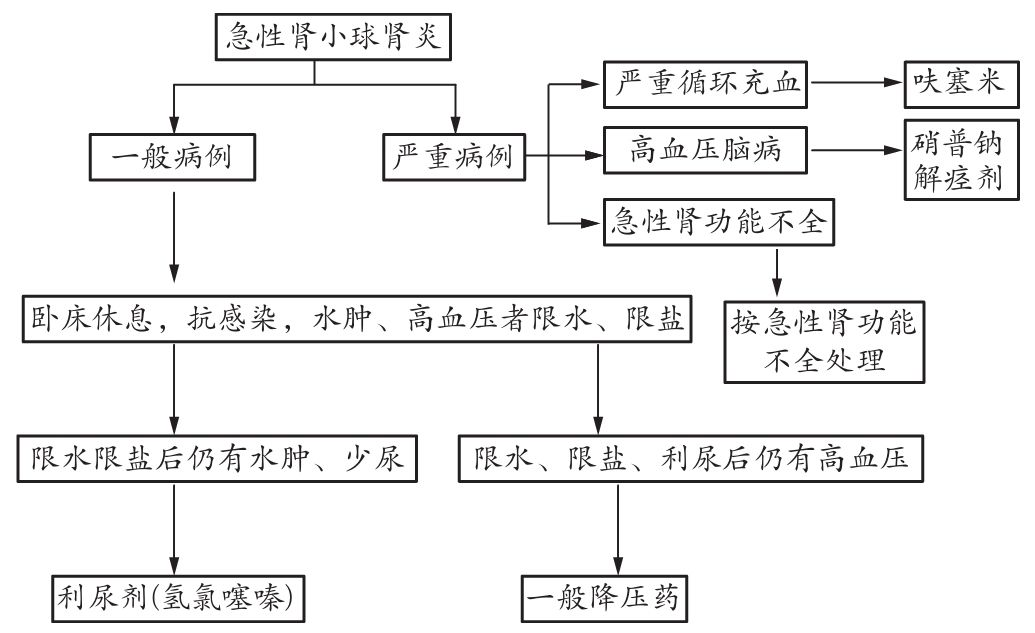
\includegraphics{./images/Image00120.jpg}
 \captionsetup{justification=centering}
 \caption{急性肾小球肾炎的治疗程序}
 \label{fig4-1-1}
  \end{figure} 

【治疗方案】 本病是自限性疾病。以对症治疗为主,防治致死性并发症(心力衰竭、急性肾衰竭、脑病),其中尤以预防和治疗水钠潴留、控制循环血容量为主。

1. 一般治疗

(1)基本卧床休息,直至肉眼血尿消失,利尿消肿,血压恢复正常。肉眼血尿消失、血清肌酐正常后可进行轻微活动。

(2)予富有维生素的低盐饮食,蛋白质摄入量保持约1g/(kg·d)。如出现肾功能不全,应限制蛋白质入量,予优质蛋白(牛奶、鸡蛋等)为主。急性期应予低盐(每日3g以下)饮食。

2. 药物治疗

(1)治疗感染灶,以往主张病初注射青霉素10\textasciitilde{}14日,但其必要性现有争议,如病灶细菌培养阳性则应积极使用抗生素,青霉素800万U+生理盐水100ml,静脉滴注,每日1次,连用2周或治愈。一般不主张长期预防性使用抗生素。反复发作的慢性腭扁桃体炎,待病情稳定后[尿蛋白少于(+),尿沉渣红细胞少于10个/Hp]应考虑作腭扁桃体摘除,术前、术后2周需注射青霉素。

(2)利尿,用于限水限盐、卧床后仍有水肿明显、少尿、血压增高的患者。可选用下列利尿剂:

双氢克尿噻25\textasciitilde{}50mg,口服,每日2\textasciitilde{}3次。呋塞米20\textasciitilde{}40mg,口服或静脉注射,每日1\textasciitilde{}3次。使用期间需监测水电解质平衡,注意大剂量呋塞米可能引起听力及肾脏的严重损害。

(3)利尿后高血压控制仍不满意时,可加用下列降压药物:

钙通道阻滞剂:下列制剂可选用一种:①尼群地平,10\textasciitilde{}20mg,口服,每日2\textasciitilde{}3次。②氨氯地平(络活喜),5\textasciitilde{}10mg,口服,每日1次。③非洛地平缓释片(波依定),5\textasciitilde{}10mg,口服,每日1次。④硝苯地平控释片(拜新同),30\textasciitilde{}60mg,口服,每日1次。

肼屈嗪,10\textasciitilde{}25mg,口服,每日3\textasciitilde{}4次。

高血压危象或高血压脑病,选用下列一种制剂予静脉滴注降压治疗,根据血压调整滴速:①硝酸甘油10mg+5\%葡萄糖注射液250ml,每分钟5μg开始。②硝普钠50mg+5\%葡萄糖注射液250ml,每分钟0.1μg/kg开始。③尼卡地平10mg+5\%葡萄糖注射液250ml,每分钟0.5\textasciitilde{}6μg/kg开始。使用期间需监测血压。

3.
透析治疗 急性肾衰竭、急性左心衰竭、高钾血症等予利尿消肿降压治疗后症状无明显改善者可行肾替代治疗。透析指征:①急性肺水肿。②高钾血症,血钾在6.5mmol/L以上。③血尿素氮21.4mmol/L以上或血肌酐442μmol/L以上。④高分解代谢状态,血肌酐每日升高超过176.8μmol/L或血尿素氮每日超过8.9mmol/L,血钾每日上升1mmol/L以上。⑤无明显高分解代谢,但无尿2日以上或少尿4日以上。⑥酸中毒,二氧化碳结合力低于13mmol/L,pH\textless{}7.25。⑦少尿2日以上,伴有下列情况任何一项者:体液潴留,如眼结膜水肿、心音呈奔马律、中心静脉压增高;尿毒症症状,如持续呕吐、烦躁、嗜睡;高血钾,血钾\textgreater{}6.0mmol/L,心电图有高钾改变,应及时给予透析治疗以帮助患者渡过急性期。同时严格控制液体入量,每日液体入量=前一日尿量+不显性失水(每日10\textasciitilde{}15ml/kg)+吐泻丢失量-内生水量(每日100ml/m{2}
)。由于本病具有自愈倾向,肾功能多可逐渐恢复,一般不需要长期维持透析。根据患者肾功能、心功能等情况,如明显好转可停止肾替代治疗。

【疗效观察与随访】

1.
观察指标 治疗后观察尿量、血压、水肿的变化。监测血沉、补体、肾功能、尿常规等指标。严重患者注意观察心率、呼吸、血压、肾功能、电解质、血常规、动脉血气等指标。

2.
治愈标准 2周左右水肿消退,血压正常,尿量正常,4\textasciitilde{}6周尿常规检查基本正常为治愈。少数患者镜下血尿可持续6个月至1年或更久。本病预后良好,痊愈率90\%\textasciitilde{}95\%。严重病例死亡率\textless{}1\%\textasciitilde{}2\%,转为慢性肾炎者\textless{}2\%。如在病程4周时少尿、高血压仍无改善甚至加重,应高度怀疑急进性肾炎。

3. 随访 密切观察病情变化,定期复查血压、尿常规、肾功能等。

【治疗经验与解析】

1.
典型病例、恢复顺利者不必进行肾活检。具有以下情况之一者可进行肾活检:少尿1周以上或进行性尿量减少伴肾功能恶化者;病程超过2个月而无好转趋势者;急性肾炎综合征伴肾病综合征者;持续低补体血症\textgreater{}8周;持续蛋白尿、血尿\textgreater{}6个月。

2. 此病好发于儿童,应积极治疗,以免病情延续发展为慢性肾炎、肾衰竭。

3.
急性期应卧床休息3周,应待血压正常,其他症状消失后,方可逐渐增加活动;3个月后可上学;6个月内避免重体力劳动。

4.
急性期若有水肿、少尿、血压高者应适当限制盐、水与蛋白质的摄入,水肿消退可以由低盐饮食逐渐过渡到普通饮食,多食用一些含维生素A、维生素C、维生素D、维生素B的食物。降压过程中考虑其血压升高主要由于水钠潴留所致的容量依赖性高血压,首选利尿剂降压,如效果不佳再联用其他类降压药。

5.
预防呼吸道感染与皮肤感染,积极治疗急性扁桃体炎、猩红热及脓疱疮等疾病。

6.
少尿\textgreater{}1周,无尿\textgreater{}3日,应警惕急性肾功能衰竭,需密切观测肾功能、电解质、动脉血气等指标,必要时行肾替代治疗,并可行肾活检明确诊断。

\subsection{急进性肾小球肾炎}

急进性肾小球肾炎是指一组病情发展急骤、由蛋白尿、血尿迅速发展为少尿或无尿性急性肾衰竭、预后恶劣的肾小球肾炎。临床表现为肉眼血尿、蛋白尿、贫血、急速进展至肾衰竭。原发性急进性肾炎分三型:①抗肾小球基底膜型(Ⅰ型),血清抗肾小球基底膜抗体阳性;②免疫复合物型(Ⅱ型),常伴肾病综合征,血循环免疫复合物及冷球蛋白可呈阳性,并可伴血清补体C3降低;③非免疫复合物型(Ⅲ型),可有不明原因的发热、乏力、体重下降、肌痛、关节痛或咯血等系统性血管炎的表现,可有血清ANCA(抗中性粒细胞胞浆抗体)阳性。肾活检病理示50\%以上肾小球有大新月体形成可确诊。

【治疗程序】 如图\ref{fig4-1-2}所示。

\begin{figure}[!htbp]
 \centering
 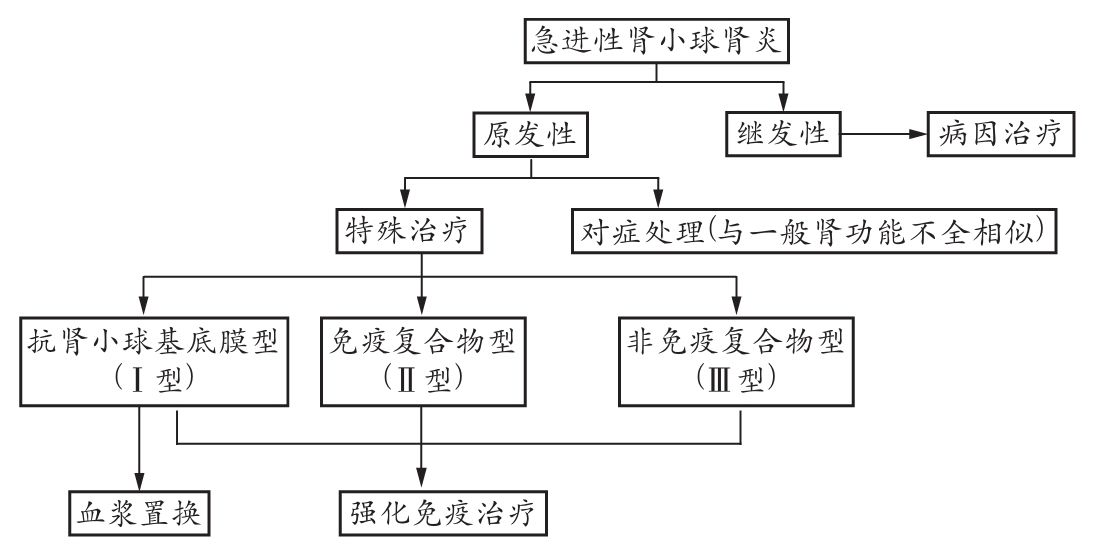
\includegraphics{./images/Image00121.jpg}
 \captionsetup{justification=centering}
 \caption{急进性肾小球肾炎的治疗程序}
 \label{fig4-1-2}
  \end{figure} 

【治疗方案】 急性期治疗的关键在于尽早诊断,明确本病诊断后,尚应区别特发性或继发性,重视本病的基本病因诊断甚为重要,因为各种疾病引起急进性肾炎的预后不同,且治疗方法和效果也异。明确诊断后充分治疗,及时采取针对免疫反应及炎症过程的强化抑制措施,且本病治疗方案主要取决于免疫病理分型。

1.
一般治疗 包括对高血压、水钠潴留、酸中毒、电解质紊乱、尿毒症及感染、心功能不全、心包炎等治疗。其方法与处理与一般肾功能不全相似。

2. 药物治疗及特殊治疗

(1)起病早期治疗,适用于各型急进性肾炎患者,Ⅰ型效果不明确。甲泼尼龙琥珀酸钠500mg+生理盐水100ml,静脉滴注,每日1次连续3日。必要时可间隔3\textasciitilde{}5日重复1个疗程。

(2)抗肾小球基底膜抗体阳性、肺出血、ANCA相关小血管炎发病时表现为急性肾衰竭可行血浆置换。每次新鲜血浆或5\%白蛋白置换2\textasciitilde{}4L患者血浆,每日或隔日1次。

(3)强化免疫治疗后可予醋酸泼尼松(龙)片1mg/(kg·d),口服,每日1次。同时可联合环磷酰胺免疫治疗,方案为环磷酰胺0.6\textasciitilde{}1.0g+生理盐水100ml,静脉滴注,每月1次连续6个月或至病情缓解。使用环磷酰胺时需定期监测血常规、肝肾功能,累积量不超过6\textasciitilde{}8g。

(4)抗凝和抗血小板聚集,双嘧达莫片,75mg,口服,每日3次,使用该药物时有患者会出现头痛,可适当减少剂量;拜阿司匹林,100mg,口服,睡前;低分子肝素(速碧林或法安明),4100\textasciitilde{}5000IU,皮下注射,每日1次。

(5)凡急性肾衰竭已达到透析指征,予以及时透析,血液透析和腹膜透析均可,晚期病例及肾功能已无法逆转者需长期维持透析。

【疗效观察与随访】

1.
观察指标 治疗后观察尿量、血压、水肿的变化。监测肾功能、电解质、血常规、凝血功能、尿常规等指标。抗肾小球基底膜型(Ⅰ型)需检测其血清抗肾小球基底膜抗体滴度,非免疫复合物型(Ⅲ型)需定期检测ANCA的浓度。

肾活检指征:临床怀疑为急进性肾小球肾炎时需积极创造条件行肾活检明确其病理类型,如细胞性新月体为主可予积极激素冲击+免疫治疗,如纤维性新月体为主免疫治疗不宜过于积极,防止发生感染等一系列并发症。

2. 疗效判定

治愈标准:症状、体征消失,病因解除,相关检测指标恢复正常,半年内未复发。

好转标准:症状、体征减轻,病因未能完全解除,部分指标仍时有不正常。

3.
随访 密切观察病情变化,定期检测相关指标,一旦发现病情变化,应及时诊治。

【治疗经验与解析】

1.
急进性肾小球肾炎起病急,预后凶险,临床治疗效果欠佳,且行血浆置换费用昂贵,需向患者及家属交代相关事宜。血浆置换应尽早开始。抗肾小球基底膜抗体阳性者行此项治疗至抗体转阴为止,如出现少尿或无尿、血肌酐\textgreater{}600μmol/L、肾活检中有大量纤维性新月体形成可考虑停止血浆置换。总体来说预后Ⅰ型最差,Ⅱ型和Ⅲ型相对较好。主要影响预后的因素包括新月体病变的新旧程度,发病时血肌酐水平以及临床上是否出现少尿和无尿等。

2.
使用大剂量糖皮质激素冲击治疗时易出现以下并发症:电解质紊乱、骨质疏松、消化道溃疡出血、感染、精神紊乱、血糖异常、肥胖等,如有必要可间隔3\textasciitilde{}5日重复1个疗程,一般不超过3个疗程。

\subsection{慢性肾小球肾炎}

慢性肾小球肾炎简称慢性肾炎,系指蛋白尿、血尿、高血压、水肿为基本临床表现,起病方式各有不同,病情迁延,病变缓慢进展,可有不同程度的肾功能减退,最终将发展为慢性肾衰竭的一组肾小球病。仅有少数慢性肾炎是由急性肾炎发展所致(直接迁延一年以上或临床痊愈若干年后再发)。绝大多数慢性肾炎的确切病因尚不清楚,起病即属慢性,约50\%的终末期肾衰患者(行双侧肾切除)证实为原发性肾小球疾病,组织学改变提示局灶节段性硬化为28\%,非特异性肾小球肾炎为28\%,系膜增生性为25\%,广泛新月体疾病为15\%,严重膜性肾小球肾炎(MGN)为4\%。另细菌及病毒感染尤其是乙型肝炎病毒感染亦可引起慢性肾炎。由于本组疾病的病理类型及病期不同,主要临床表现可各不相同,疾病表现呈多样化,治疗困难,预后较差。一般人群中发病率不明,但在尸检中占0.5\%\textasciitilde{}1\%。

【治疗程序】 如图\ref{fig4-1-3}所示。

\begin{figure}[!htbp]
 \centering
 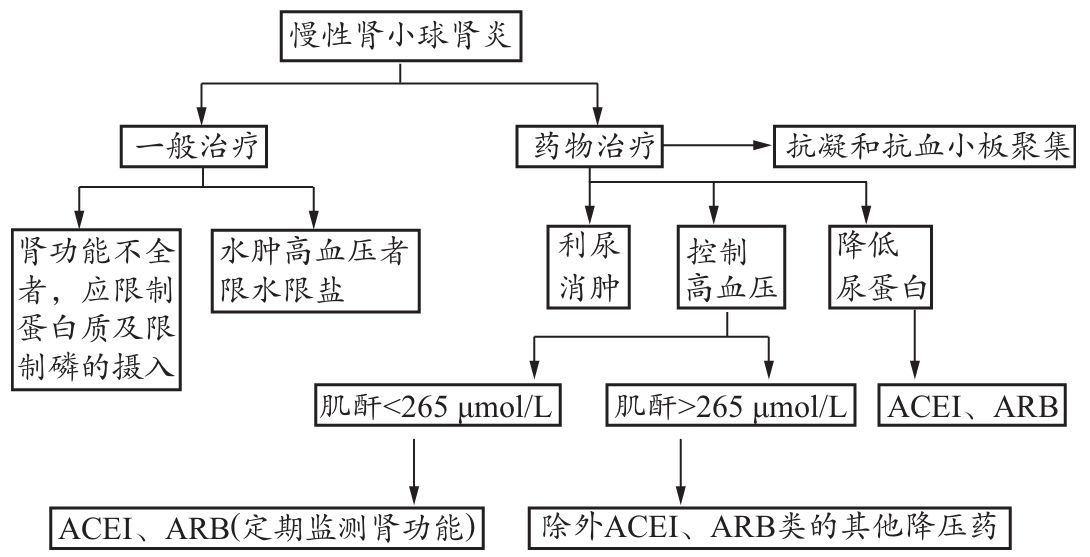
\includegraphics{./images/Image00122.jpg}
 \captionsetup{justification=centering}
 \caption{慢性肾小球肾炎的治疗程序}
 \label{fig4-1-3}
  \end{figure} 

【治疗方案】 以防止或延缓肾功能进行性恶化、改善或缓解临床症状及防治严重合并症为主要目的,尽可能降低尿蛋白。

1.
一般治疗 肾功能正常者,有大量蛋白尿,可适当放宽蛋白摄入量,但不超过1.0g/(kg·d)。肾功能不全者应限制磷的摄入量(\textless{}600mg/d),并予优质低蛋白饮食,每日30\textasciitilde{}40g,辅以必需氨基酸(复方α-酮酸片,开同)口服。水肿及血压高的患者应限盐。

2. 药物治疗

(1)利尿消肿:用于限水限盐、卧床后仍有水肿明显、少尿、血压增高的患者。可选用下列利尿剂:①噻嗪类利尿剂:双氢克尿噻25\textasciitilde{}50mg,口服,每日2\textasciitilde{}3次(适用于肾功能正常的患者);②襻利尿剂,呋塞米20\textasciitilde{}40mg,口服或静脉注射,每日1\textasciitilde{}3次(适用于其他利尿剂效果不佳以及肾功能不全的患者)。③潴钾利尿剂:螺内酯,20mg,口服,每日3次(单独使用效果不佳,适合与噻嗪类合用)。使用利尿剂需监测水电解质平衡,注意大剂量呋塞米可能引起听力及肾脏的严重损害。

(2)控制高血压:

1)血肌酐265μmol/L以下的患者首选ACEI和(或)ARB。

下列ACEI制剂可选用1种:贝那普利(洛汀新)10\textasciitilde{}40mg,口服,每日1次;福辛普利(蒙诺)5\textasciitilde{}40mg,口服,每日1次;培哚普利(雅施达)2\textasciitilde{}4mg,口服,每日1次;卡托普利(开搏通)6.25\textasciitilde{}25mg,口服,每日2次。

下列ARB制剂可选用1种:氯沙坦(科素亚)50\textasciitilde{}100mg,口服,每日1次;缬沙坦(代文)80\textasciitilde{}160mg,口服,每日1次;厄贝沙坦(安博维)150\textasciitilde{}300mg,口服,每日1次。

2)其他降压药物:适合单用ACEI和(或)ARB血压控制不理想以及使用ACEI、ARB有禁忌证的患者,根据血压水平选择以下一种或几种药物联合应用:①钙通道阻滞剂(下列制剂可选用1种):尼群地平10\textasciitilde{}20mg,口服,每日2\textasciitilde{}3次;氨氯地平(络活喜)5\textasciitilde{}10mg,口服,每日1次;非洛地平缓释片(波依定)5\textasciitilde{}10mg,口服,每日1次;硝苯地平控释片(拜新同)30\textasciitilde{}60mg,口服,每日1次。②利尿剂(同上)。③β受体阻滞剂(下列制剂可选用1种):美托洛尔片(倍他乐克)6.25\textasciitilde{}25mg,口服,每日2次;美托洛尔缓释片(倍他乐克缓释片)47.5mg,口服,每日1次。④肾上腺素受体阻滞剂:阿罗洛尔(阿尔马尔)5\textasciitilde{}10mg,口服,每日1\textasciitilde{}2次;卡维地洛片(金络)6.25\textasciitilde{}12.5mg,口服,每日1\textasciitilde{}2次。⑤血管扩张剂:肼屈嗪10\textasciitilde{}25mg,口服,每日3\textasciitilde{}4次。

(3)降低尿蛋白:可选用任一种长效ACEI和(或)ARB(用法同上)。

(4)抗凝和抗血小板聚集:双嘧达莫片75mg,口服,每日3次;拜阿司匹林100mg,口服,睡前;低分子肝素(速碧林或法安明)4100\textasciitilde{}5000IU,皮下注射,每日1次。

(5)中药辅助治疗:可选用雷公藤10\textasciitilde{}20mg,口服,每日3次;百令胶囊4\textasciitilde{}5粒,口服,每日3次;黄葵胶囊4\textasciitilde{}5粒,口服,每日3次;肾炎康复片5\textasciitilde{}8粒,口服,每日3次。

【疗效观察与随访】

1.
观察指标 治疗后观察尿量、血压、水肿的变化。监测肾功能、电解质、尿常规、血常规、24小时尿蛋白定量、24小时尿NAG酶等指标。

肾活检指征:因慢性肾小球肾炎病理类型较多,且轻重不等,临床上无明显禁忌证者皆可以行肾活检以明确诊断,判断预后,指导下一步治疗。

2. 疗效判定

治愈标准:症状、体征消失,相关检测指标均恢复正常,半年内未复发。

好转标准:症状、体征减轻,部分指标未能完全恢复正常。

3. 随访 密切观察病情变化 特别是肾功能变化,一旦恶化,必须及时处理。

【治疗经验与解析】

1.
本病治愈较困难,除药物治疗外,饮食治疗及劳逸结合十分重要,饮食上要低盐饮食,不要服损害肾功能之药物,如止痛片、某些对肾有损害的抗生素等,并要注意避免受凉感冒诱发肾炎复发。

2.
本病的治疗应尽可能减少尿蛋白,但不以消除尿蛋白为目标,故一般不主张应用激素和细胞毒药物。如患者肾功能正常或轻度受损,肾脏体积正常,尿蛋白\textgreater{}2.0g/24h,病理类型为轻度系膜增生性肾炎、轻微病变等病变较轻者,如无禁忌证可试用激素和细胞毒药物,无效者逐步撤去。如果使用激素治疗,应系统服药,开始剂量充足,尿蛋白阴性后逐渐减量,以至停服,但切勿突然停服,否则易反跳复发。在服用激素治疗过程中,始终要注意防治感染的发生。

3.
慢性肾小球肾炎患者的血压控制标准为:蛋白尿\textgreater{}1g/d,血压应控制在125/75mmHg以下;尿蛋白\textless{}1g/d,血压控制可放宽到130/80mmHg以下。使用ACEI和(或)ARB类药物时需密切监测血肌酐值的动态变化,如用药后血肌酐上升,上升值低于原来的30\%可继续应用,超过原来的50\%者应停用,在30\%\textasciitilde{}50\%之间者可在严密监测下继续应用,肾功能不全者要监测血钾,以防止发生高钾血症。

\subsection{肾病综合征}

肾病综合征是由多种病因、病理和临床疾病所引起的一组症状群,包括:①尿蛋白超过3.5g/d。②血浆白蛋白低于30g/L。③水肿。④血脂升高。其中①②两项是诊断所必需的。可分为原发性及继发性两大类,可由多种不同病理类型的肾小球疾病引起。临床上首先明确病因,必须除外继发性和遗传性疾病,才能诊断为原发性肾病综合征。行肾活检可确定其病理类型明确诊断。引起原发性肾病综合征的肾小球病主要病理类型为微小病变型肾病、系膜增生性肾小球肾炎、系膜毛细血管性肾小球肾炎、膜性肾病及局灶节段性肾小球硬化。

肾病综合征患者临床常易发生各种并发症,注意观测:①感染。②血栓、栓塞并发症。③急性肾衰竭。④营养不良、生长发育迟缓等。

【治疗程序】 如图\ref{fig4-1-4}所示。

\begin{figure}[!htbp]
 \centering
 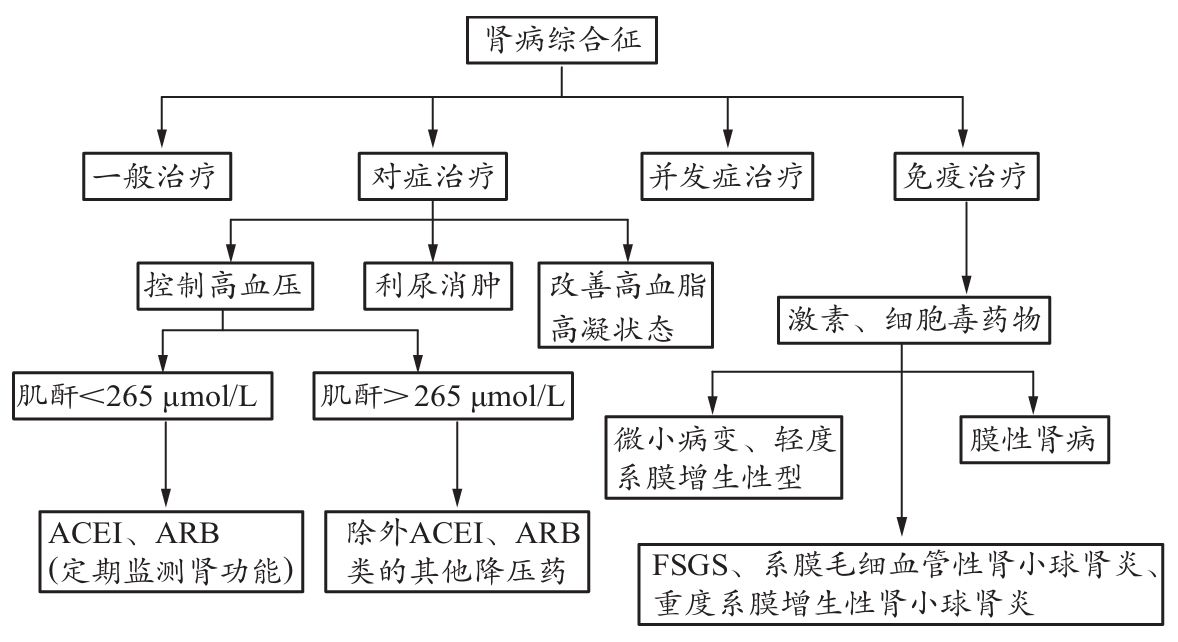
\includegraphics{./images/Image00123.jpg}
 \captionsetup{justification=centering}
 \caption{肾病综合征的治疗程序}
 \label{fig4-1-4}
  \end{figure} 

注意:使用糖皮质激素及细胞毒药物时需根据病理类型及临床症状选用合适的剂量及类型,注意监测药物的副作用

【治疗方案】 本病的治疗以减少尿蛋白、提高血浆白蛋白为目标,同时需注意对症治疗及合并症的治疗。

1.
一般治疗 卧床休息为主,减少与外界接触防止发生交叉感染。但应适度保持床上及床旁活动,防止肢体血栓形成。饮食宜低盐、低脂、优质低蛋白,胃肠道粘膜水肿严重时需进易消化、清淡、半流质饮食。

2. 对症治疗

(1)利尿消肿:用于限水限盐、卧床后仍有水肿明显、少尿、血压增高的患者。可选用下列利尿剂:①噻嗪类利尿剂:双氢克尿噻25\textasciitilde{}50mg,口服,每日2\textasciitilde{}3次(适用于肾功能正常的患者);②襻利尿剂,呋塞米20\textasciitilde{}40mg,口服或静脉注射,每日1\textasciitilde{}3次(适用于其他利尿剂效果不佳以及肾功能不全的患者)。③潴钾利尿剂:螺内酯20mg,口服,每日3次(单独使用效果不佳,适合与噻嗪类合用)。使用利尿剂需监测水电解质平衡,注意大剂量呋塞米可能引起听力及肾脏的严重损害。

(2)控制高血压:

1)血肌酐265μmol/L以下的患者首选ACEI和(或)ARB:

下列ACEI制剂可选用1种:贝那普利(洛汀新)10\textasciitilde{}40mg,口服,每日1次;福辛普利(蒙诺)5\textasciitilde{}40mg,口服,每日1次;培哚普利(雅施达)2\textasciitilde{}4mg,口服,每日1次;卡托普利(开搏通)6.25\textasciitilde{}25mg,口服,每日2次。

下列ARB制剂可选用1种:氯沙坦(科素亚)50\textasciitilde{}100mg,口服,每日1次;缬沙坦(代文)80\textasciitilde{}160mg,口服,每日1次;厄贝沙坦(安博维)150\textasciitilde{}300mg,口服,每日1次。

2)其他降压药物:适合单用ACEI和(或)ARB血压控制不理想以及使用ACET、ARB有禁忌证的患者,根据血压水平选择以下一种或几种药物联合应用:①钙通道阻滞剂(下列制剂可选用1种):尼群地平10\textasciitilde{}20mg,口服,每日2\textasciitilde{}3次;氨氯地平(络活喜)5\textasciitilde{}10mg,口服,每日1次;非洛地平缓释片(波依定)5\textasciitilde{}10mg,口服,每日1次;硝苯地平控释片(拜新同)30\textasciitilde{}60mg,口服,每日1次。②利尿剂(同上)。③β受体阻滞剂(下列制剂可选用1种):美托洛尔片(倍他乐克)6.25\textasciitilde{}25mg,口服,每日2次;美托洛尔缓释片(倍他乐克缓释片)47.5mg,口服,每日1次。④肾上腺素受体阻滞剂:阿罗洛尔(阿尔马尔)5\textasciitilde{}10mg,口服,每日1\textasciitilde{}2次;卡维地洛片(金络)6.25\textasciitilde{}12.5mg,口服,每日1\textasciitilde{}2次。⑤血管扩张剂:肼屈嗪10\textasciitilde{}25mg,口服,每日3\textasciitilde{}4次。

(3)改善高血脂、高凝状态(下列制剂可选用1种):氟伐他汀(来适可)40\textasciitilde{}80mg,口服,睡前;阿托伐他汀钙(立普妥)20\textasciitilde{}40mg,口服,睡前;辛伐他汀(舒降之)20\textasciitilde{}40mg,口服,睡前。

3.
主要治疗 应用糖皮质激素及细胞毒类药物抑制免疫与炎症反应,应根据肾脏病变的病理类型制定用药方案。

(1)微小病变和轻度系膜增生性肾小球肾炎的患者选用:

1)糖皮质激素:泼尼松或泼尼松龙1mg/(kg·d)清晨1次顿服,维持8\textasciitilde{}12周。有效者逐渐减量,每2\textasciitilde{}3周减原用药量的5\%\textasciitilde{}10\%,减至每日10\textasciitilde{}15mg时,改为隔日顿服(即将2日总量隔日清晨1次顿服),继续减至最小有效剂量作为维持量,再服半年至1年或更长。

根据对糖皮质激素的治疗反应,可将患者分为“激素敏感型”(用药8周内肾病综合征缓解)、“激素依赖型”(激素减量到一定程度即复发)和“激素抵抗型”(激素治疗无效)三类。

2)细胞毒类免疫抑制剂:适用于“激素依赖型”、“激素抵抗型”的患者或反复发作的患者,与糖皮质激素联合治疗,常用环磷酰胺。①环磷酰胺2mg/(kg·d),分1\textasciitilde{}2次口服,或200mg每日或隔日静脉注射1次,或600mg每2周静脉注射1次,累积量达6\textasciitilde{}8g后停药。②氮芥由1mg开始,隔日静注1次,每次加量1mg,至5mg后每周注射2次,累积量达1.5\textasciitilde{}2.0mg/kg时停药。

3)环孢素A(CsA):作为二线药物,适用于激素及细胞毒药物无效的难治性肾病综合征。CsA5mg/(kg·d)分2次口服,服药2\textasciitilde{}3个月后缓慢减量,共服半年左右。

4)麦考酚酸酯(骁悉,MMF):适用于难治性肾病综合征。初始剂量1.5g/d,分2次口服,维持3个月;维持剂量1.0g/d,分2次口服,维持3\textasciitilde{}6个月。

(2)膜性肾病的患者选用:

1)特发性膜性肾病在伴有肾病综合征时强调观察基础治疗6个月,尿蛋白约\textgreater{}4g/d和超过维持在高于基线水平50\%以上,且无下降趋势,开始应用糖皮质激素和烷化剂(CTX)6个月的交替治疗方案。

2)钉突形成后的膜性肾病是否仍用激素和细胞毒药物正规治疗尚无一致意见,若治疗,则疗程完成后,无论尿蛋白是否减少均应果断减药,以免发生严重副作用。

(3)局灶节段性肾小球硬化、系膜毛细血管性肾小球肾炎、重度系膜增生性肾小球肾炎,肾功能正常的患者选用:先给足量激素和细胞毒药物,可同时加用抗凝药和抗血小板药,疗程完成后无论疗效如何均及时减药,以避免严重不良反应;随后保持维持量激素和抗血小板药长期服用。

1)联合应用足量糖皮质激素和细胞毒药物,用法同微小病变和轻度系膜增生性肾小球肾炎。

2)抗凝药:低分子肝素钙(速碧林)4100IU,或低分子肝素钠(法安明)5000IU,皮下注射,每日1次,疗程为2\textasciitilde{}3个月。

3)抗血小板药双嘧达莫(潘生丁)50\textasciitilde{}75mg,口服,每日3次。

(4)肾功能不全的患者:①不再给予糖皮质激素及细胞毒药物治疗。②按“慢性肾功能不全”处理。

4. 并发症的治疗

(1)血栓栓塞并发症的防治:

1)当血浆白蛋白浓度低于20g/L时,提示高凝状态的存在,即应开始预防性抗凝治疗:①抗凝剂:维持凝血时间长于正常1倍。低分子肝素钙(速碧林),4100IU,或低分子肝素钠(法安明)5000IU,皮下注射,每日1次。②抗血小板药:双嘧达莫(潘生丁)100mg,每日3次;或阿司匹林50\textasciitilde{}300mg,每日1次。

2)已发生血栓栓塞者应尽早溶栓治疗,6小时内最佳,但3日内仍可望有效,可全身或局部给药:尿激酶2万\textasciitilde{}6万U+5\%葡萄糖溶液100ml,缓慢静注或静滴,每日1次,1\textasciitilde{}2周为1个疗程。

(2)并发急性肾衰竭:①原发病的治疗。②襻利尿剂,呋塞米。③血液透析,利尿无效并已达透析指征者采用。④碱化尿液,减少管型的形成。

【疗效观察与随访】

1.
观察指标 治疗后观察尿量、血压、水肿的变化。监测肾功能、肝功能、凝血功能、电解质、血清蛋白电泳、尿圆盘电泳、尿常规、血常规、24小时尿蛋白定量、24小时尿NAG酶等指标。如系继发性肾病综合征,需注意观测原发病的相关指标。

肾活检指征:因肾病综合征病理类型较多,且轻重不等,临床上无明显禁忌证者皆可以行肾活检以明确诊断,判断预后,指导下一步治疗。

2.
疗效评价 显效:症状、体征明显减轻,肾功能逐步恢复,相关检测指标有明显改善,但尿蛋白、肌酐仍时有增加。

3.
随访 密切观察病情变化,尤其是水肿,蛋白尿及肌酐的变化,坚持定期复查,定期门诊诊治。

【治疗经验与解析】

1.
本病是一个复杂的病理生理过程,对其治疗应经过严密的临床观察个性化处置,治疗过程中应严密监测药物的不良反应。

2.
使用利尿剂治疗时需注意水电解质平衡,且利尿不宜过快过猛,否则造成血容量不足、血液高粘度,从而诱发血栓、栓塞性并发症。噻嗪类利尿剂可导致血尿酸增高,不适合已有高尿酸血症的患者。潴钾利尿剂与噻嗪类合用,可加强利尿效果,并减少电解质紊乱。少尿患者应用渗透性利尿剂有诱发“渗透性肾病”导致急性肾衰竭的风险,应慎用。另患者处于低血容量状态时可考虑应用血浆或白蛋白联合利尿剂治疗,但不应频繁使用血浆制品,因白蛋白输入后24\textasciitilde{}48小时内即经尿液全部排出,增加肾小球滤过负担,增加近曲小管蛋白重吸收负担,加重其上皮细胞空泡变性。

3.
使用ACEI和(或)ARB类药物时需密切监测血肌酐值的动态变化,如用药后血肌酐上升,上升值低于原来的30\%可继续应用,超过原来的50\%者应停用,在30\%\textasciitilde{}50\%之间者可在严密监测下继续应用,肾功能不全者要监测血钾,以防止发生高钾血症。

4.
服用降血脂药物时坚持低胆固醇饮食;定期检查肝功能;孕妇及哺乳期妇女禁用;肌毒性是他汀类药物安全性的重要方面,一旦发生肌无力或肌痛就应立即停药,严重肾功能不全患者使用他汀类药物时血药浓度会增加,发生肌病和横纹肌溶解的危险也增加,对于慢性肾脏疾病患者应根据肾小球滤过率调整剂量。

5.
对于继发性肾病综合征如乙型肝炎病毒相关性肾炎、糖尿病肾病等需慎用激素。应用糖皮质激素治疗成功的关键在于起始剂量要足够,大剂量诱导用药时间要充分,有效者减药速度要慢。当减量至20mg/d左右时症状易反复,应更加缓慢减量。如患者水肿严重、有肝功能损害或泼尼松疗效不佳时,可更换为泼尼松龙(等剂量)口服或静滴。长期应用激素的患者易出现感染、骨质疏松、药物性糖尿病等不良反应,少数患者还可能发生股骨头无菌性缺血性坏死,需注意预防,加强监测,及时处理。

6.
使用免疫抑制剂时需向患者交代可能出现的毒副反应:①环磷酰胺主要为中毒性肝损害和骨髓抑制,并可出现性腺抑制、脱发、胃肠道反应和出血性膀胱炎、月经紊乱、无精子或精子减少及肺纤维化等并发症。如因不良反应不能用环磷酰胺者,建议改用骁悉。②氮芥因有较强的局部组织刺激作用、严重的胃肠道反应和骨髓抑制作用,目前临床应用较少,但在其他细胞毒药物无效时可考虑选用。给药前先用镇静止吐药,静脉注射毕续滴5\%GS100\textasciitilde{}200ml冲洗血管以防静脉炎。③服用环孢素A期间需监测血药浓度,维持其谷值在100\textasciitilde{}200ng/ml。

\subsection{IgA肾病}

IgA肾病是一种常见的原发性肾小球疾病,特征为反复发作的肉眼血尿或镜下血尿,系膜区IgA沉积或以IgA沉积为主,是肾小球源性血尿最常见的病因。常在感染后出现肉眼血尿,血清中IgA1显著升高,IgA1结构异常。可发生在任何年龄,16\textasciitilde{}35岁的患者占总发病人数的80\%。临床表现多种多样,轻重不一,从无症状血尿到肾病综合征、高血压、急进性肾炎乃至肾功能不全。病理表现为:弥漫性系膜细胞增生、系膜外基质增多,轻重不一,各类型均可见到;IgA为主的免疫球蛋白在系膜区呈颗粒样或团块样沉积伴有C3沉积。由于其临床表现及病理表现多种多样,轻重不一,治疗时需结合两者来制定相应的方案。

【治疗程序】 如图\ref{fig4-1-5}所示。

\begin{figure}[!htbp]
 \centering
 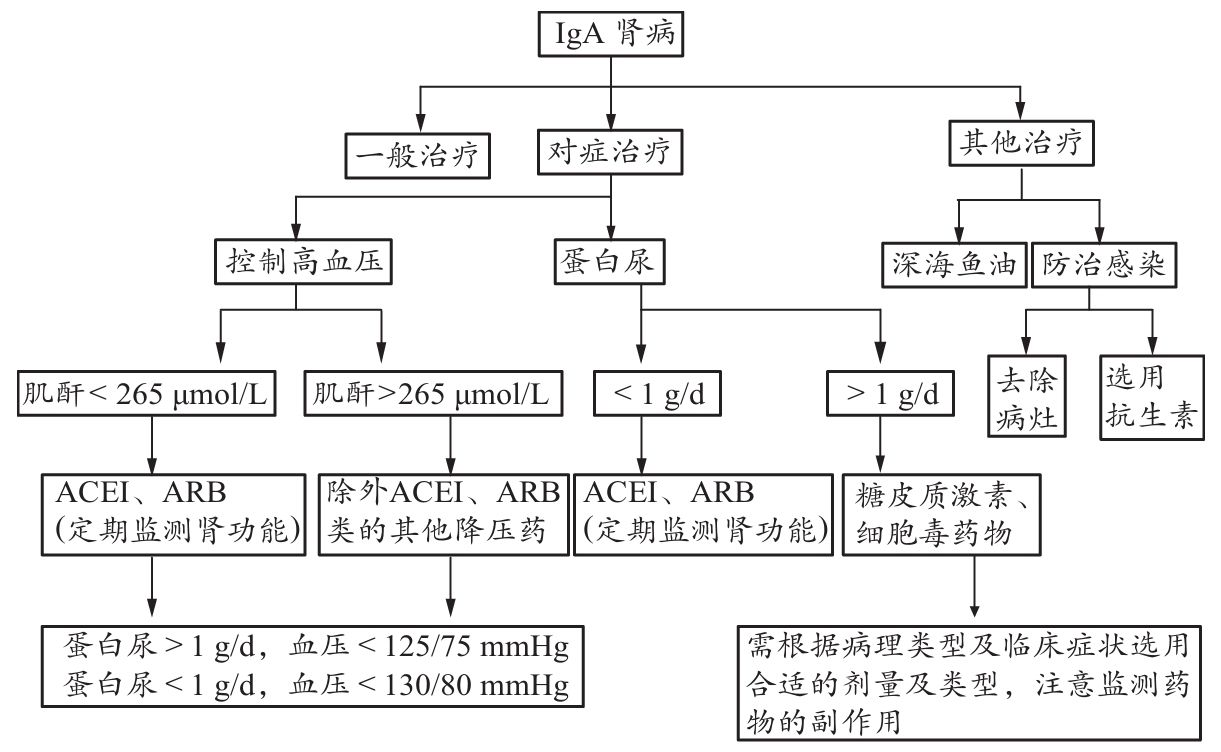
\includegraphics{./images/Image00124.jpg}
 \captionsetup{justification=centering}
 \caption{IgA肾病的治疗程序}
 \label{fig4-1-5}
  \end{figure} 

【治疗方案】

1.
一般治疗 控制感染,IgA肾病肉眼血尿常和上呼吸道感染同时发生,提示感染刺激可诱发IgA肾病,因此积极治疗和去除口咽部、上颌窦的感染灶对减少肉眼血尿的发作应该有益。同时避免使用肾毒性药物、避免过度劳累。有高血压时需限制盐的摄入。

2. 药物治疗

(1)控制高血压:

1)血肌酐265μmol/L以下的患者首选ACEI和(或)ARB。

下列ACEI制剂可选用1种:贝那普利(洛汀新)10\textasciitilde{}40mg,口服,每日1次;福辛普利(蒙诺)5\textasciitilde{}40mg,口服,每日1次;培哚普利(雅施达)2\textasciitilde{}4mg,口服,每日1次;卡托普利(开搏通)6.25\textasciitilde{}25mg,口服,每日2次。

下列ARB制剂可选用1种:氯沙坦(科素亚)50\textasciitilde{}100mg,口服,每日1次;缬沙坦(代文)80\textasciitilde{}160mg,口服,每日1次;厄贝沙坦(安博维)150\textasciitilde{}300mg,口服,每日1次。

2)其他降压药物:适合单用ACEI和(或)ARB血压控制不理想以及使用ACET、ARB有禁忌证的患者,治疗方面,参见高血压节。

(2)合并蛋白尿的治疗:

1)正常肾功能、微量蛋白尿\textless{}0.5g/d、血压正常、肾组织病变轻微,不需治疗,定期随访。

2)正常肾功能、蛋白尿0.5\textasciitilde{}1g/d,血压正常,应用鱼油和ACEI或ARB降尿蛋白。

3)正常或轻微肾功能损害,蛋白尿\textgreater{}1g/d,鱼油和ACEI或ARB降尿蛋白\textless{}1g/d,3\textasciitilde{}6个月无效,GFR\textgreater{}50ml/min,建议6个月的糖皮质激素治疗。

4)肾病综合征表现:轻微病变的给予40\textasciitilde{}60mg/d泼尼松治疗;病变重者强的松疗程延长并联合细胞毒药物治疗。

5)快速进展性:临床表现为急进型肾炎且病理证实为新月体性肾炎者,及早给予糖皮质激素(冲击和常规口服)、细胞毒药物、血小板解聚药,可行血浆置换治疗。静脉大剂量免疫球蛋白可能有益。

(3)深海鱼油:可减轻肾小球间质炎症、血小板凝聚和血管收缩从而延缓肾损害。

【疗效观察与随访】

1.
观察指标 监测肾功能、电解质、尿常规、尿红细胞位相、免疫球蛋白、血常规、24小时尿蛋白定量、24小时尿NAG酶等。

肾活检指征:因IgA肾病病理类型较多,且轻重不等,临床上无明显禁忌证者皆可以行肾活检以明确诊断,判断预后,指导下一步治疗。

2. 疗效评价 显效:症状与体征减轻,相关检测指标改善。

3.
随访 密切观察病情变化,定期复查尿常规、肾功能、免疫球蛋白及24小时尿NAG酶等。

【治疗经验与解析】

1.
IgA肾病是一类慢性迁延性疾病,其临床表现及肾功能状态不断缓慢地变化,是ESRD的重要诱因之一。其临床和病理表现多样,轻重不一,诊断和治疗时需明确影响IgA肾病预后的危险因子:肾功能受损、高血压、大量蛋白尿、肾小球硬化和间质纤维化等,这些因子是IgA肾病最强和最可靠的预后不良指标。

2.
对于IgA肾病合并蛋白尿者:蛋白尿\textgreater{}1g/d,血压应控制在125/75mmHg以下;尿蛋白\textless{}1g/d,血压控制可放宽到130/80mmHg以下。使用ACEI和(或)ARB类药物时需密切监测血肌酐值的动态变化,如用药后血肌酐上升,上升值低于原来的30\%可继续应用,超过原来的50\%者应停用,在30\%\textasciitilde{}50\%之间者可在严密监测下继续应用,肾功能不全者要监测血钾,以防止发生高钾血症。

\subsection{隐匿性肾小球肾炎}

隐匿性肾小球肾炎也称为无症状性血尿或(和)蛋白尿,患者无水肿、高血压及肾功能损害,而仅表现为蛋白尿或(和)肾小球性血尿。多数患者是在体格检查或在偶然情况下尿常规检查发现异常,而无症状、体征。多种不同的基础疾病其临床特征均可表现为隐匿性肾炎。肾活检是明确诊断的唯一可靠方法。本组疾病由多种病理类型的原发性肾小球病所致,但病理改变多较轻。如可见于轻微病变性肾小球肾炎(肾小球中仅有节段性系膜细胞及基质增生)、轻度系膜增生性肾小球肾炎及局灶性节段性肾小球肾炎(局灶性肾小球病,病变肾小球内节段性内皮及系膜细胞增生)等病理类型。

【治疗方案】

1.
一般治疗 控制吸烟、适当限制饮食中蛋白质的量、防治感冒、预防过敏以及控制腭扁桃体炎,对反复发作的慢性腭扁桃体炎与血尿、蛋白尿发作密切相关者,可待急性期过后行腭扁桃体摘除术。

2. 药物治疗

(1)ACEI和(或)ARB:

下列ACEI制剂可选用1种:贝那普利(洛汀新)10\textasciitilde{}40mg,口服,每日1次;福辛普利(蒙诺)5\textasciitilde{}40mg,口服,每日1次;培哚普利(雅施达)2\textasciitilde{}4mg,口服,每日1次;卡托普利(开搏通)6.25\textasciitilde{}25mg,口服,每日2次。

下列ARB制剂可选用1种:氯沙坦(科素亚)50\textasciitilde{}100mg,口服,每日1次;缬沙坦(代文)80\textasciitilde{}160mg,口服,每日1次;厄贝沙坦(安博维)150\textasciitilde{}300mg,口服,每日1次。

(2)抗凝和抗血小板聚集:双嘧达莫片75mg,口服,每日3次;拜阿司匹林100mg,口服,睡前;低分子肝素(速碧林或法安明)4100\textasciitilde{}5000IU,皮下注射,每日1次。

(3)中药辅助治疗:可选用百令胶囊4\textasciitilde{}5粒,口服,每日3次;黄葵胶囊4\textasciitilde{}5粒,口服,每日3次;肾炎康复片5\textasciitilde{}8粒,口服,每日3次。

【疗效观察与随访】

1.
观察指标 监测肾功能、电解质、尿常规、血常规、24小时尿蛋白定量、24小时尿NAG酶等。

肾活检指征:因隐匿性肾炎病理类型较多,且轻重不等,临床上无明显禁忌证者皆可以行肾活检以明确诊断,判断预后,指导下一步治疗。

2. 治愈标准 症状、体征消失,相关检测指标正常,半年未复发。

3.
随访 密切观察病情变化,定期复查尿常规、肾功能、24小时尿蛋白定量及尿NAG酶。

【治疗经验与解析】

1.
对于血压正常的患者使用ACEI和(或)ARB类药物时需监测其血压的动态变化,如血压过低或患者有不适主诉,可适当减量。

2.
对于非肾病综合征水平的蛋白尿是否需要使用糖皮质激素治疗的问题目前还没有定论。治疗期间患者应定期(至少每3个月1次)检查,监测尿沉渣、肾功能和血压的变化,女患者在妊娠前及其过程中更需加强监测;同时注意保护肾功能、避免肾损伤的因素。

\section{继发性肾小球肾病}

\subsection{糖尿病肾病}

糖尿病肾病(diabetic
nephropathy,DN)是1型和2型糖尿病最常见的慢性并发症之一,也是当今糖尿病患者致残和致死的重要原因。在美国,糖尿病肾病是导致终末期肾衰竭的首要病因,在我国,糖尿病肾病的发病率也逐年上升。糖尿病肾病对肾脏的损害几乎累及肾脏所有结构,包括肾小球、肾小管、肾间质及肾血管等,糖尿病肾病作为糖尿病的血管并发症之一,不仅在临床表现和疾病进程方面和其他免疫介导的肾脏疾病不同,而且一旦出现肾功能损害,其进展速度亦远快于非糖尿病肾病患者。而且,临床观察发现,糖尿病肾病进展至终末期时,无论是透析还是肾移植,远期预后均比其他肾病差。目前,随着社会经济发展和生活水平的提高,糖尿病肾病已成为影响人类健康的一个重大问题。

【治疗方案】

1.
一般治疗 加强宣教和监测对糖尿病及其并发症的控制来说尤为重要。大部分糖尿病患者本来就是自我控制不严,饮食和营养方式不科学,从而导致了糖尿病。糖尿病肾病大部分也是对糖尿病自身认识不足,重视程度不够所致。因此,加强宣教,让患者、家属及其他社会人群正确认识糖尿病的危害及其并发症表现,合理饮食,积极配合治疗,延缓并发症的出现和进展速度,减轻家庭和社会负担均非常有效。

饮食治疗是最为基本的治疗措施。蛋白主张量少质优的原则,选择优质动物蛋白,植物蛋白,特别是豆制品只能少量食用。糖尿病肾病饮食治疗原则:早期DN期(Ⅲ期),每日蛋白质摄入量为0.8g/kg;临床DN期(Ⅳ期),蛋白每日摄入应减至0.6g/kg,联合开同补充必需氨基酸;尿毒症期(Ⅴ期),在行肾替代治疗同时,蛋白补充不需严格限制。对于合并有肝病、妊娠及生长发育期不宜过度限制蛋白。DN患者严格饮食控制同时需提供每日足够的热量,轻体力工作糖尿病患者,每日的总热量控制在25\textasciitilde{}30kcal/kg,糖占总热量的50\%\textasciitilde{}60\%,脂肪占30\%\textasciitilde{}35\%。动物内脏、脂肪及高热量食物应少吃。

体育锻炼或体力活动非常重要,有利于增加能耗,减轻体重,提高胰岛素敏感性,从而降低血糖、血脂。延缓和减轻糖尿病的多个系统并发症。一般主张三餐后慢走30分钟,注意随身携带糖果,避免运动后低血糖发生。

2. 药物治疗

(1)控制血糖:参见糖尿病节。

(2)降脂治疗:糖尿病常并发高脂血症,一般血清胆固醇\textgreater{}5.7mmol/L,甘油三酯\textgreater{}1.7mmol/L,LDL-C\textgreater{}3.7mmol/L,应加降脂药。

以胆固醇增高为主,可选用他汀类,第一代洛伐他汀、辛伐他汀、普伐他汀,第二代氟伐他汀,第三代阿托伐他汀,睡前服用。他汀类药物除调脂作用外,还发现具有抗肾脏固有细胞增殖及基质增生作用。其主要不良反应有横纹肌肌溶解及肝脏损害,但发生率很低。

以甘油三酯为主,选用贝特类,如吉非贝特、非诺贝特等。一般要求餐后服用。不良反应同他汀类。

混合型高脂血症,在饮食和血糖控制同时,首选他汀类,他汀其和贝特类合用,会增加不良反应的发生率,一般不主张。烟酸衍生物,如阿昔莫司,可以减少VDLD及LDL合成。

(3)降压治疗:糖尿病肾病的高血压控制较非糖尿病肾病严格,如24小时尿蛋白\textgreater{}1.0g,建议血压控制在125/75mmHg以下,如24小时尿蛋白\textless{}1.0g,建议血压控制在130/80mmHg以下。

血管降压药物中ACEI或ARB能降低肾小球滤过率、改善肾内血流动力学、抑制系膜细胞、成纤维细胞及巨噬细胞活性,改善膜通透性,减少蛋白尿,因此作为DN降压首选。ACEI类国内常用的有卡托普利、贝那普利、依那普利、培哚普利和福辛普利,ARB有氯沙坦、缬沙坦、替米沙坦、厄贝沙坦等。ACEI或ARB在血压正常情况下也可对肾脏有保护作用,并不完全依赖于血流动力学改善,因此在糖尿病肾病早期,即使没有高血压,也需要使用。ACEI不良反应主要有高钾血症、肾功能恶化及干咳,ARB除了没有干咳外也和ACEI有类似的不良反应,但对肾小球滤过率的影响小于ACEI。如血清肌酐\textgreater{}3mg/d,谨慎使用,定期检查;如血清肌酐\textgreater{}4mg/d,一般不主张用,如需要使用,应严密监测血钾和肾功能的变化。

其他降压药物如钙通道阻滞剂(CCB)降压效果好,没有明显的不良反应,在ACEI或ARB单药效果不佳或不能使用时是其最佳选择,现在我们主张平稳安全降压,短效CCB降压迅速而且有效,但是其可引起反射性心率加快,易诱发DN的心血管并发症,因此一般建议选用中长效CCB联合降压。利尿剂和倍他乐克由于有干扰糖代谢的潜在风险,一般不作为首选。

(4)中医中药治疗:糖尿病属中医的消渴病范畴,传统治疗中药有天花粉、生地、麦冬、山药、黄芪、党参、黄连、葛根等,现代中医和中西医结合者根据糖尿病微血管病变,多加了活血化瘀药。近年来,许多学者还发现了黄芪、丹参、龙胆草、甘草等对醛糖还原酶有较好的抑制作用,其中分离出来的单体成分如黄芪甙、葛根素、水飞蓟宾等作用较强,能够抑制AGEs形成,减轻蛋白尿。

(5)其他治疗:如醛糖还原酶抑制剂可防治DM微血管病变,AGEs抑制剂氨基胍能抑制蛋白质非酶糖基化及蛋白间异常交联,清除氧自由基,防止脂质过氧化,改善肾内病变。

3.
终末期肾病治疗 肾替代治疗是DN终末期的最主要治疗方法,血液透析和腹膜透析均可选择。另外,也有极少部分人群可选择肾或者胰肾联合移植。

【疗效观察与随访】

1.
观察指标 尿量,尿常规,血常规,肝肾功能,血脂,电解质,血气分析,FBG,HbA1c,眼底检查,血压,内生肌酐清除率,PTH,双肾超声等。

2. 疗效评估 显效:症状、体征明显减轻,相关检测指标改善,病情较稳定。

3.
随访 密切观察病情变化,定期检测相关指标,注意肝肾功能及血气变化,一旦病情变化,及时复诊。

【治疗经验与解析】

1.
对于早期糖尿病肾病,各类口服降糖药物均可以使用,一般不需减量。在达到临床糖尿病肾病期时,肾小球滤过率下降,降糖药物在体内会蓄积,代谢减慢从而引起顽固性低血糖,同时许多降糖药物经肾脏代谢,加重肾脏负担,有一定的肾毒性,这时主张选用胰岛素治疗。相对来说糖适平、达美康、拜糖平、诺和龙是常用的口服降血糖药物,安全性较高。糖尿病肾病患者在使用胰岛素控制血糖时也需要根据患者的肾功能水平来选择剂量,由小剂量缓慢加量。对于血液透析患者,在透析前(一般指当日)暂停1次胰岛素,透析结束如需进食,在进食前30分钟皮下注射胰岛素。糖尿病肾病由于血管条件不好选择腹膜透析也不少,腹透液中糖浓度很高,因此选择腹膜透析的DN患者,胰岛素用量需加量,有的甚至需要把胰岛素加入腹透液中来控制血糖。

2.
他汀类和贝特类可能引起转氨酶升高,一般停药后可恢复。偶可发生严重的横纹肌溶解综合征,若出现肌痛等症状可监测血肌酸磷酸激酶(CPK)和血肌红蛋白。

3.
ACEI和ARB易引起高钾血症,因此使用时要求饮食限钾,一般不合并用补钾或可致血钾升高的其他药物。因ACEI或ARB均能减少肾小球灌注,因此在使用这两种药物之前,必须评价患者饮食好坏,双肾动脉有无狭窄等情况,只有在排除以后才可以谨慎使用,否则药物引起肾脏灌注不足,加重肾损害。如在使用这两种药物过程出现血肌酐上升过快(半月内上升超过基础值的30\%),建议停药观察。

4.
糖尿病肾病并发症多,症状出现早且重,应适当放宽透析指征,一般内生肌酐清除率小于15ml/min,或伴有明显胃肠道症状,高血压、心衰不易控制者即可进入维持性透析。

5.
血液透析与腹膜透析的长期生存率相近,前者血糖容易控制,透析充分性好,但内瘘建立比较困难,透析过程中易发生心脑血管意外;而腹膜透析心脑血管并发症少,不需建立内瘘,对中大分子清除较好,在家里操作比较方便,但存在血糖不易控制,操作不当容易感染等风险。

\subsection{狼疮性肾炎}

系统性红斑狼疮(systemic lupus
erythematosus,SLE)是侵犯皮肤和全身多脏器的一种自身免疫性疾病。从发病机理来看,遗传因素只是一种易感倾向,环境因素在本病的促发中起重要作用,如病毒感染,药物因素,以及日光(紫外线)照射等。狼疮性肾炎(lupus
nephritis,LN)是我国最常见的继发性肾小球疾病之一,也是导致SLE患者死亡的主要原因,是系统性红斑狼疮最常见和最重要的内脏并发症。我国LN发病率高,随着社会工业化,环境污染加重,有不断升高的趋势。几乎所有SLE患者的肾组织均有病理变化,但仅约75\%有临床表现。多数肾受累发生于发热、关节炎、皮疹等肾外表现之后,重型病例病变常迅速累及浆膜、心、肺、肝、造血器官和其他脏器组织,并伴相应的临床表现。约1/4的患者以肾脏损害为首发表现。

【治疗程序】 如图\ref{fig4-2-1}所示。

\begin{figure}[!htbp]
 \centering
 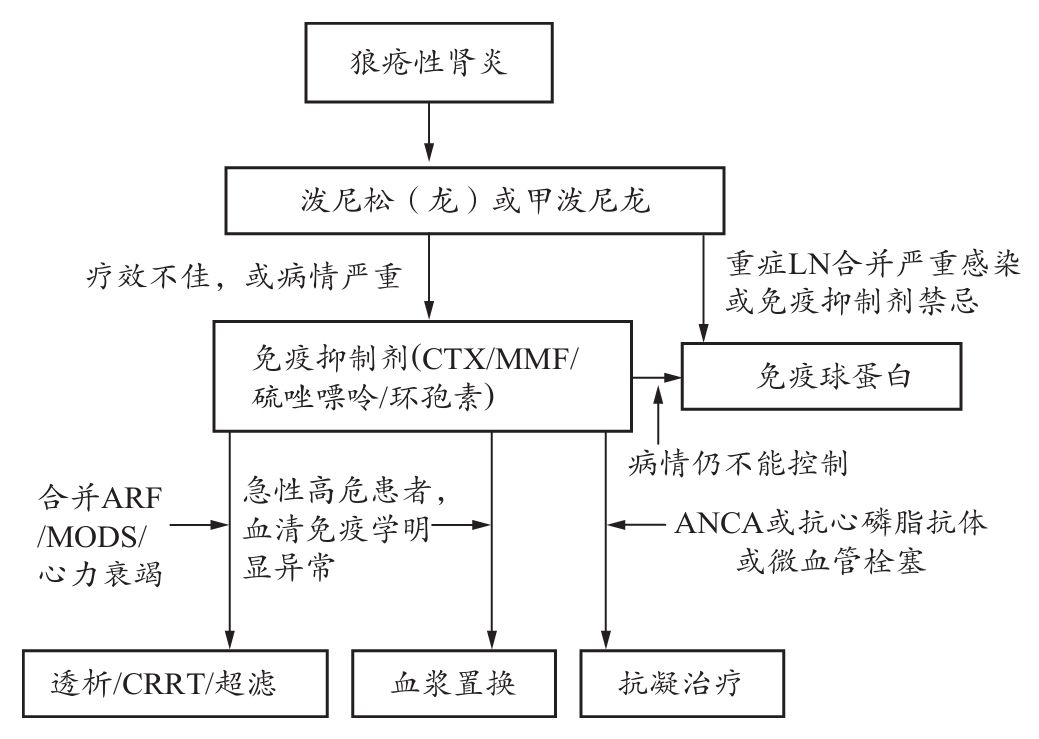
\includegraphics{./images/Image00125.jpg}
 \captionsetup{justification=centering}
 \caption{狼疮性肾炎的治疗程序}
 \label{fig4-2-1}
  \end{figure} 

【治疗措施】 按病情轻重,病变类型,活动度及肾功能状况制订治疗方案。

1.
一般治疗 急性期或活动期应卧床休息,卧室用深色窗帘以避阳光。慢性稳定期可室内工作,避免过劳和暴晒于强阳光下。即使有轻度感染也应及时积极治疗。诱发或可加重病情的药物(如肼屈嗪、甲基多巴、苯妥英钠及磺胺药等)不宜使用。建议任何LN都应使用羟氯喹,每天最大剂量6\textasciitilde{}6.5mg/kg。女性妊娠期可继续使用,LNⅢ型或以上者应加肾小球肾炎治疗原则的一般治疗。

2. 药物治疗

(1)糖皮质激素:对病理上属Ⅰ\textasciitilde{}Ⅲ型者(轻度系膜增生,无坏死和新月体形成),开始服泼尼松30\textasciitilde{}40mg,以后观察病情变化,以决定下一步剂量;对SLE急性活动期,患者有发热,关节痛明显,蛋白尿中量以上及肾活检Ⅲ\textasciitilde{}Ⅳ型LN,且活动性指数\textgreater{}11分,泼尼松以1mg/(kg·d)为宜,取效后可较快地减至40mg/d,然后每1\textasciitilde{}2周减去5mg,用10\textasciitilde{}15mg/d维持时改为隔日晨1次服用,病情稳定,可再减量,长期糖皮质激素治疗,应加服小剂量雌激素、钙剂及维生素D,以防骨质疏松。对严重肾病综合征或急进性LN,或伴狼疮脑病者,可采用激素冲击疗法。

(2)免疫抑制剂:对重症SLE和LN一般均加用免疫抑制剂,单用糖皮质激素不易获得完全和持续缓解,且减量易复发或出现糖皮质激素副作用。Ⅲ型、Ⅳ型LN建议采取环磷酰胺(CTX)或霉酚酸酯(MMF)加泼尼松初始治疗6月。如发热、皮损及关节症状明显者,为了迅速控制症状需用大剂量激素,若加用CTX则可减少糖皮质激素的剂量,既可取得同样效果,又可避免长期大剂量激素的副作用。美国国立卫生研究院(NIH)的总结证明,SLE或LN口服泼尼松和CTX或硫唑嘌呤合用取得良效。CTX冲击治疗每3个月1次,合用泼尼松的疗效肯定,超过单用泼尼松的疗效。近年来,对LN活动期大多采用糖皮质激素或CTX冲击疗法,方法是甲泼尼龙0.5\textasciitilde{}1.0g,每日或隔日静脉滴注,共3次;CTX冲击剂量为0.6\textasciitilde{}1.0g,开始每半个月1次,2次后改每个月1次,6个月后隔月或每3个月1次,共用2年,对肾功能减退者CTX应减量,静脉用药的间歇期,隔日用泼尼松40mg,对急进性LN及狼疮脑等重危病例,采用糖皮质激素-CTX双冲击疗法,在治疗过程中感染为主要并发症。MMF的初始治疗剂量为2g/d,共治疗6月。

维持治疗可用硫唑嘌呤1.5\textasciitilde{}2.5mg/(kg·d)或MMF1\textasciitilde{}2g/d与激素合用,LN孕妇如病情活动主张用大剂量激素和硫唑嘌昤,因为CTX孕妇禁用。

环孢素对LN有一定疗效,通常剂量为3\textasciitilde{}6mg/(kg·d),分2次服用:一般用6\textasciitilde{}8周可取效,病情稳定后每月将每日量减1/4,以2mg/(kg·d)维持。由于本药对肾小管间质有毒性损害,故主张在使用上述药物无效时再考虑应用,或与其他免疫抑制剂合用,短期观察疗效满意,可使蛋白尿及血尿明显减轻,肾功能保持稳定。

3.
其他治疗 静脉滴注丙种球蛋白0.2\textasciitilde{}0.4g/kg,每日或隔日1次,连用5\textasciitilde{}10日,可使SLE及LN症状缓解,蛋白尿显著减少或消失。由于丙种球蛋白封闭了单核巨噬细胞的Fc受体,抑制自身抗体的产生,并可溶解免疫复合物。国外报道有效率可达80\%,本疗法仅适用于重症LN且对激素及CTX禁忌或产生显著副作用,或有严重感染者。雷公藤多苷对SLE及LN有一定疗效,如与激素合用或单独使用,一般10\textasciitilde{}20mg,每日3次。

4.
对症治疗 治疗盘状红斑狼疮可用氯喹类,如氯喹0.25g或羟氯喹0.2g,每日1次服用,本药能减弱抗体对抗原的吸附能力,稳定溶酶体膜,故有抗过敏、抗炎及减轻组织损害作用;对SLE患者的光过敏及皮疹和关节疼痛也有一定效果。

SLE易发生血管及组织微血管血栓形成,尤其是血清抗磷脂抗体或ANCA阳性者,应采用防治措施,如低分子量肝素(如速碧林0.4ml,皮下注射每日1次)、硫酸肝素、尿激酶,小剂量阿司匹林或双嘧达莫也可做预防之用。

5.
血液净化 对急性高危患者,血清免疫学明显异常者可考虑采用血浆置换,合并急性肾功能衰竭者应及早进行血液透析,如伴有心力衰竭或多脏器衰竭者采用持续肾脏替代治疗。

6.
LN复发的治疗 对完全或部分缓解后复发的LN患者建议用原来治疗有效的初始治疗及维持治疗。若重复使用原治疗方案将导致CTX过量,推荐用不含CTX的初始治疗方案。若怀疑患者的肾脏病理类型发生变化,或不能确定SCr升高,蛋白尿恶化是活动性病变还是慢性病变所致,可考虑重复肾活检。

【疗效观察与随访】

1.
观察指标 治疗后观察皮疹、关节疼痛、浆膜腔积液等的改善情况。定期复查患者的血常规、尿常规、血沉、肝肾功能、补体、自身抗体的变化。

2. 治愈标准:症状、体征消失,相关检测指标恢复正常,肾功能恢复半年以上。

3. 随访 密切观察病情变化,定期复查血、尿常规、血沉、肝肾功能、抗体等。

【治疗经验与解析】

1.
无肾穿刺禁忌者应尽早行肾活检明确病理类型,及早进行针对性治疗,可明显改善预后。

2.
应严格掌握糖皮质激素应用指征,用药过程中密切随访,及时防治副作用,包括严重感染(病毒、细菌、真菌和活动性结核等),严重的骨质疏松,严重糖尿病,严重高血压,精神病,青光眼,病毒性肝炎。

3. 治疗过程中,出现感染应及时使用强有力的抗感染治疗。

4. 使用激素及免疫抑制剂过程中,注意定期监测血常规、肝肾功能。

5. 免疫抑制剂多对胎儿有不良影响,孕妇慎用。

6.
对一些严重LN如有大量新月体形成、合并栓塞性微血管病变,或抗核抗体/ANCA高滴度阳性,或弥漫性肺泡出血者,可采用血浆置换或免疫吸附治疗。

7.
由于持续缓解病例也可能在若干年后复发,所以一般不主张完全停用免疫抑制治疗。通常可以采取小剂量激素维持。对不能遵从长期药物治疗的患者,可以考虑在持续缓解至少5年以后再停止药物治疗,但必须密切观察患者尿液检查和免疫学指标变化。

8.
大量蛋白尿伴肾炎综合征、高血压、治疗前血肌酐已升高者预后不好。病理改变与预后的关系最为密切,Ⅰ型和Ⅱ型一般不发展为终末期肾病;Ⅲ型可有病情活动性发展,但治疗反应好,5年存活率可达75.8\%;Ⅳ型病情多危重,但如及时、正确治疗,5年存活率可达80\%,10年存活率60\%;Ⅴ型不伴有明显增生时预后同原发性膜性肾病,但若伴有明显或较明显的增生性病变则预后不好,与Ⅳ型相似。影响狼疮性肾炎预后的因素还有病变活动程度:病变持续活动或反复活动者的预后较非活动病例差;病因:病因不明者预后差,药物引起者停药后病变迅速好转,预后良好;治疗是否早期进行,是否充分控制活动期,均直接影响预后。本病是一种反复发作,逐渐进展的肾脏病,临床经过差异较大。自从应用大剂量肾上腺皮质激素及并用免疫抑制剂以来,本病预后已有改观,存活率有所提高。

\subsection{紫癜性肾炎}

过敏性紫癜(HSP)是一种常见的血管变态反应性出血性疾病,皮肤、关节、胃肠道及肾脏是本病受累的主要器官。以坏死性小血管炎为基本病变,伴IgA免疫球蛋白/复合物沉积于皮肤小血管及肾小球系膜区、内皮下,使血管通透性和脆性增加,导致皮下组织、粘膜及内脏器官出血、水肿。紫癜性肾炎(HSPN)是过敏性紫癜的肾损害,是一种常见的继发性肾小球肾炎。过敏性紫癜患者约1/3以上出现肾炎,其预后主要取决于肾病的严重程度。常表现为血尿、蛋白尿,部分患者可伴高血压和肾功能不全。HSPN患者可因致敏原性质不同、个体反应性差异及血管炎累及的器官和病变程度不同,在临床和肾脏病理上呈现不同的改变,对治疗的反应和预后也有较大差异。

本病常发生于10岁以下儿童,成年人中少见。好发生于寒冷季节。约1/3患者有细菌、病毒等先驱感染史,约1/4患者与鱼、虾类过敏或预防注射、药物有关。大多数患者呈良性、自限性过程,多于数周内痊愈。但也有反复发作或迁延数周、数月者。约50\%患者病程反复发作。

【治疗程序】 如图\ref{fig4-2-2}所示。

\begin{figure}[!htbp]
 \centering
 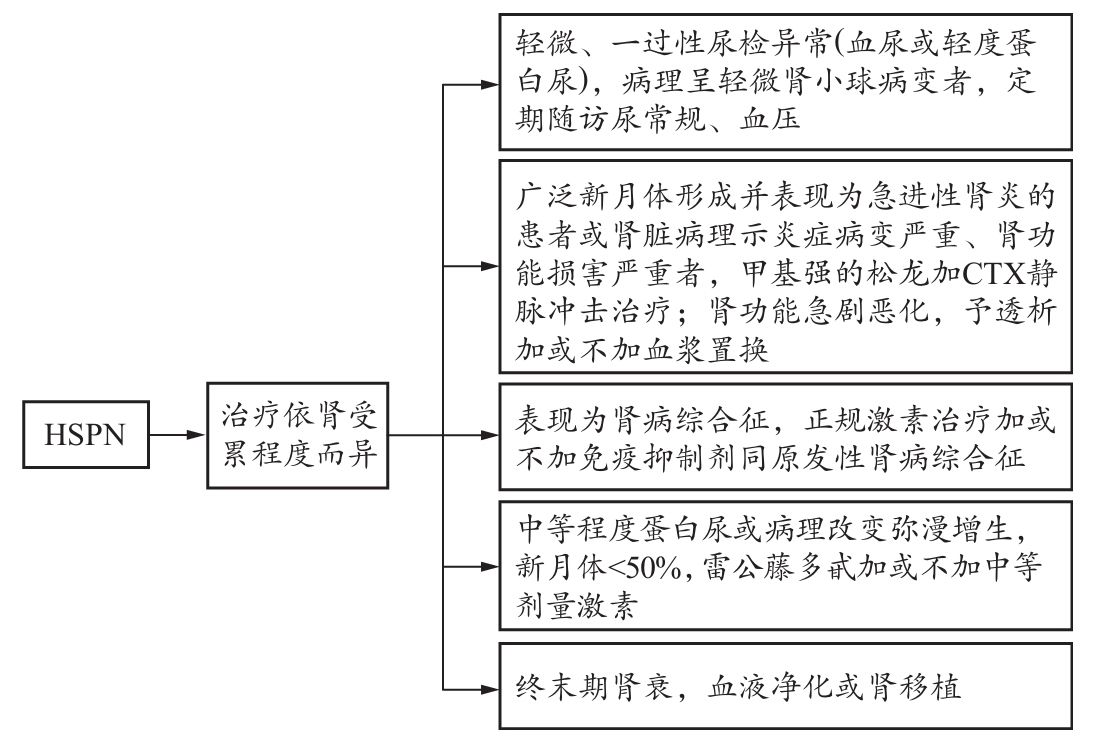
\includegraphics{./images/Image00126.jpg}
 \captionsetup{justification=centering}
 \caption{紫癜性肾炎的治疗程序}
 \label{fig4-2-2}
  \end{figure} 

【治疗方案】

1.
一般治疗 急性期应卧床休息、注意保暖、停用可疑过敏药物及食物,避免接触可疑过敏原。

2. 药物治疗

(1)抗组胺类药物:尿蛋白轻度改变、镜下血尿、轻微尿蛋白,肾功能正常,肾活检呈轻微改变或局灶性增生改变时,可用抗组胺药如克敏能(氯雷他定)10mg/d或静脉钙剂10\%葡萄糖酸钙10\textasciitilde{}20ml静脉推注,每日1\textasciitilde{}2次;改善血管通透性药物如维生素C
5\textasciitilde{}10g/d静滴,持续5\textasciitilde{}7日。

(2)糖皮质激素:临床表现为急性肾炎综合征、肾病综合征、急进性肾炎,病理改变为系膜增生性肾炎伴局灶或弥漫性大细胞新月体或呈膜增生性肾炎,主张糖皮质激素治疗。已予ACEI或ARB治疗,蛋白尿仍持续\textgreater{}1g/(d·1.73m{2}
),GFR\textgreater{}50ml/(min·1.73m{2}
)的患者,也建议采用糖皮质激素治疗。对缓解胃肠道、关节肿痛症状也可短期应用。泼尼松初始剂量0.6\textasciitilde{}1.0mg/(kg·d),服用8周后逐渐减量,每2\textasciitilde{}4周减10\%,逐渐减量至隔日顿服,维持量为隔日5\textasciitilde{}10mg,总疗程6\textasciitilde{}12个月以上。广泛新月体形成并表现为急进性肾炎的患者或肾脏病理示炎症病变严重、肾功能损害严重者,首选甲泼尼龙冲击治疗,剂量小儿15\textasciitilde{}30mg/(kg·d),成人0.5\textasciitilde{}1.0g/d,静脉滴注3日,根据病情需要可追加1疗程,间歇期及疗程结束后,改为泼尼松口服0.6\textasciitilde{}1.0mg/(kg·d),并逐渐减量。

(3)免疫抑制剂:一般常与糖皮质激素联合使用,单独应用效果不佳。适用于经一般治疗无效的肾炎综合征、肾病综合征和急进性肾炎,有明显新月体形成合并肾功能不全、高血压、少尿的肾病综合征。目前常用者多为环磷酰胺CTX。用法:2\textasciitilde{}3mg/(kg·d),口服或静脉注射,疗程8\textasciitilde{}12周,口服最大量不超过200\textasciitilde{}250mg/(kg·d),静脉注射总量150mg/kg。其他制剂和剂量有:①硫唑嘌呤:2\textasciitilde{}3mg/(kg·d),分2\textasciitilde{}3次口服,疗程3个月。②苯丁酸氮芥:2mg/(kg·d)口服,疗程小于8周。③长春新碱:每次1.4mg/m{2}
,最大量每次不超过2mg,3\textasciitilde{}7日1次,尿蛋白转阴后每周1次,10次为1个疗程;④环孢素A:6\textasciitilde{}8mg/(kg·d)或100\textasciitilde{}150mg/m{2}
,同时监测浓度调整剂量,疗程2\textasciitilde{}6个月。⑤霉酚酸酯(MMF)1.0\textasciitilde{}1.5g/d,连续6个月,然后逐渐减量,总疗程9\textasciitilde{}12个月以上。⑥雷公藤多甙0.5\textasciitilde{}1.6mg/(kg·d)分3次口服,2\textasciitilde{}3个月为1疗程。

(4)RAS阻断剂:ACEI或ARB这两类药物除降压作用外,还具有减少蛋白尿、减轻肾脏炎症和纤维化的作用。无明显低血压时,可加用ACEI或ARB。

(5)抗凝治疗:对高凝状态目前尚无统一标准。有作者认为:血浆蛋白\textless{}20g/L,血浆纤维蛋白浓度\textgreater{}6g/L,抗凝血酶原浓度\textless{}70\%或和D二聚体浓度\textgreater{}1g/L,可作为高凝状态的诊断标准,应考虑抗凝治疗。常用的有肝素、蝮蛇抗栓酶、潘生丁、复方丹参等。最近使用低分子肝素皮下注射5000U,每日1\textasciitilde{}2次,持续7\textasciitilde{}10日。当肌酐清除率\textless{}20mg/min时,剂量减半,有利于肾病早期缓解,而且出血倾向小,无需特殊监护,便于临床应用。

3. 疾病进展至终末期肾衰者 可作透析及肾移植治疗。

【疗效观察与随访】

1.
观察指标 治疗后观察紫癜的变化。复查血常规、尿常规、粪便常规、血沉、肝肾功能、尿蛋白定量的变化。严重患者注意观察心率、呼吸、血压及血红蛋白的变化。

2. 治愈标准 症状、体征消失,相关指标恢复正常,3个月内未复发。

3.
随访 治疗后注意病情变化,定期复查尿常规、血沉、肝肾功能。教育患者勿再接触可疑的致敏物质。

【治疗经验与解析】

1. 紫癜性肾炎的治疗首先要避免可能致敏的食物及药物。

2.
使用糖皮质激素及免疫抑制剂时应注意其副作用,监测血常规、肝肾功能等指标。发现感染存在,早期治疗。

3. 虽然存在出血,但治疗时无需输注血小板及使用止血药物。

4.
本病发病经过可急可缓,虽经治疗,大部分可获缓解,但较易复发。约1/3的患者均出现反复发作。一般认为蛋白尿\textgreater{}2g/d,全身水肿、低蛋白血症及高血压是严重肾病变的证据,预后较差。临床仅有血尿和(或)蛋白尿者,在病理上多属轻型;出现肾病综合征、急进型肾炎或高血压者多属重型。儿童的远期转归观察发现,1.0\%\textasciitilde{}15.7\%发展至终末期肾病。

\subsection{乙型肝炎病毒相关性肾炎}

乙型肝炎病毒相关性肾炎(HBV-GN)是指由乙型肝炎病毒直接或间接诱发的肾小球肾炎,经血清免疫学及肾活检免疫荧光所证实,并除外病因明确的其他继发性肾小球肾炎(如狼疮性肾炎)的一种疾病。男性居多,儿童多见。可以表现为无症状尿检异常,也可表现为肾病范围蛋白尿,可伴有血尿。肾脏损害病理类型多样,病理:主要表现为膜性肾病,其次为系膜毛细血管性肾炎、系膜增生性肾炎、局灶节段硬化性肾炎,毛细血管内增生性肾炎偶见,儿童以膜性肾病常见,成人则多表现为膜增生性肾小球肾炎或膜性肾病。

【治疗方案】

1.
一般治疗 注意休息,避免过于劳累。防止受凉感冒或上呼吸道感染。有腭扁桃体炎、中耳炎、鼻窦炎、龋齿时应及时诊治。注意个人卫生,保持皮肤清洁,防止皮肤感染。这些都是可能导致本病复发或活动的诱因。水肿明显、大量蛋白尿而肾功能正常者可适量补充蛋白质饮食。无水肿及低蛋白血症时,每日蛋白质摄入量应限制在每公斤体重0.6克(每瓶牛奶约含6克蛋白质,每只蛋约含6克蛋白质,每50克米饭约含4克植物蛋白质)。有水肿、高血压和心功能不全者,应进低盐饮食,每日摄盐应少于3克。表现为肾病综合征者,可予以利尿剂、静脉补充白蛋白等非特异利尿消肿治疗。如无禁忌,可给予血管紧张素转换酶抑制剂或血管紧张素受体拮抗剂降低蛋白尿治疗。

2. 药物治疗

(1)抗病毒治疗:一线用药为普通干扰素-α(1b,2a及2b)和聚乙二醇化干扰素-α(2a和2b),但后一类疗效更高。

1)α-干扰素:可选用下列任何一种:①重组人干扰素α1b:每次30\textasciitilde{}50μg,每日1次,皮下或肌内注射。连用4周后改为隔日1次,疗程4\textasciitilde{}6个月,可根据病情延长疗程至1年。适合治疗伴有HBV-DNA阳性的成年患者。②重组人干扰素-α2a:每次450万IU,每周3次,皮下注射,共用6个月。如用药1个月后病毒复制标志或HBeAg无下降,则可逐渐加大剂量并可进一步将剂量调整至患者能够耐受的水平,如治疗3\textasciitilde{}4个月后没有改善,则应考虑停止治疗。适合治疗伴有HBV-DNA,HBeAg及DNA多聚酶阳性等病毒复制标志的成年患者。③重组人干扰素α2b:皮下或肌内注射,每日300万\textasciitilde{}600万IU,连用4周后改为每周3次,连用16周以上。适合治疗伴有HBV-DNA阳性的成年患者。

2)聚乙二醇化干扰素α2a:每次180μg,每周1次,共48周,腹部或大腿皮下注射。适用于治疗成人慢性乙型肝炎,患者不能处于肝病失代偿期,慢性乙型肝炎必须经过血清标志物(AST、ALT、HBsAg,HBV-DNA)确诊。

3)拉米夫定:口服:成人每次0.1g,每日1次。适用于乙型肝炎病毒复制的慢性乙型肝炎。

4)阿德福韦酯:口服,成人每次10mg,每日1次。适用于乙型肝炎病毒活动复制证据、并伴有ALT或AST持续升高或肝脏组织学活动性病变的肝功能代偿的成年慢性乙型肝炎患者。

5)恩替卡韦:适用于病毒复制活跃、血清ALT持续升高或肝脏组织学显示有活动性病变的慢性成人乙型肝炎。口服,应空腹服用(餐前或餐后至少2小时)。①成人每次0.5mg,每日1次。拉米夫定治疗时病毒血症或出现拉米夫定耐药突变的患者为每日1次,每次1mg。②肾功能不全:肌酐清除率\textless{}50ml/min(包括接受血液透析或CAPD治疗的患者)应根据肌酐清除率的值调整用药剂量:30\textasciitilde{}50ml/min者:每日1次,每次0.25mg;拉米夫定治疗失效(1.0mg)者,每日1次,每次0.5mg。10\textasciitilde{}30ml/min者:每日1次,每次0.15mg;拉米夫定治疗失效(1.0mg)者,每日1次,每次0.3mg。血液透析或CAPD者:每日1次,每次0.15mg;拉米夫定治疗失效(1.0mg)者,每日1次,每次0.3mg。血液透析后用药。

6)替比夫定:适用于有乙型肝炎病毒活动复制证据、并伴有ALT或AST持续升高或肝脏组织学活动性病变的肝功能代偿的成年慢性乙型肝炎。口服:①成人(包括≥16岁的青少年):每日1次,每次600mg。②肾功能不全:肌酐清除率≥30\textasciitilde{}49ml/min者,每次600mg,每48小时1次;肌酐清除率\textless{}30ml/min(无须透析)者,每次600mg,每72小时1次;终末期肾病患者,每次600mg,每96小时1次,应在血液透析完后服用。

(2)免疫抑制剂治疗:适用于蛋白尿、水肿严重的病例。首选霉酚酸酯(MMF)。常用量为每日1.5\textasciitilde{}2g,分2次口服,共用3\textasciitilde{}6个月,减量维持半年。有报道说MMF联合小剂量糖皮质激素能降低蛋白尿,副作用少,但缺乏大规模临床验证资料。目前不主张单独使用糖皮质激素。

【疗效观察与随访】

1.
观察指标 包括两个方面,一是乙肝病毒活动性指标,如HBV-DNA;二是肾小球肾炎相关指标,如尿蛋白定量、尿红细胞、肾功能等。几乎全部患者血HBsAg阳性,部分病例HBeAg阳性。可伴有血清C3、C4降低,冷球蛋白增多,白蛋白减少,胆固醇轻度增高,ALT、AST可增高。

2.
治愈标准 该病难以彻底治愈,如果尿蛋白小于0.4g/24h,血尿消失,肾功能正常,维持3年不复发,可视为临床痊愈。机体感染乙型肝炎病毒常难以清除,但经治疗后应力求肝功能维持正常水平。

3.
随访 密切观察病情变化,定期复查乙肝病毒活动性指标、肾小球肾炎相关指标等,随访至少为3年。

【治疗经验与解析】

1.
使用抗病毒治疗期间应对患者的临床情况及病毒学指标进行定期检查。任何一种干扰素对于过敏体质,特别是对抗生素有过敏者,应慎用。在使用过程中如发生过敏反应应立即停药,并给予相应治疗。

2.
干扰素有骨髓抑制作用,使白细胞,特别是粒细胞、血小板减少,其次是血红蛋白的降低,从而增加感染及出血的危险性。故在治疗之前及治疗中的适当时期对这些项目进行密切监测,并定期进行全血计数检查。其他常见不良反应:发热、疲乏、头痛、肌痛、关节痛等,常出现在用药后第1周,不良反应多在注射48小时后消失。

3. 抗病毒治疗的药物对儿童的安全及疗效尚未定论,故不推荐儿童使用。

4.
使用免疫抑制剂治疗,需要警惕用药后可能导致严重感染的副作用,尤其肾功能不全的患者。

5.
干扰素治疗乙型肝炎的具有一定的有效率,目前存在的主要问题是停药后复发率较高,因此疗程时间相对较长,以降低复发率。

\subsection{抗中性粒细胞胞浆抗体相关性小血管炎肾损害}

本病是西方国家最为常见的自身免疫性疾病之一,在我国尚无确切流行病学资料,其发病率尚不清楚。随着抗中性粒细胞胞浆抗体(ANCA)在我国的推广应用,对该类疾病日益重视,认识也在提高。按照受累血管的大小分为大血管炎、中血管炎和小血管炎。其中部分小血管炎与ANCA相关,又称为ANCA相关小血管炎(AASV),主要包括肉芽肿性多血管炎(GPA)、显微镜下型多血管炎(MPA)和变应性肉芽肿性血管炎(CSS)。临床上可累及多个脏器,肾脏受累多表现为少免疫沉积性坏死性新月体性肾炎。临床上肺肾可同时或先后受累,多进展迅速,严重者可危及患者生命,但早期诊断、及时合理治疗往往可逆转病情,挽救患者生命。

【治疗程序】 如图\ref{fig4-2-3}所示。

\begin{figure}[!htbp]
 \centering
 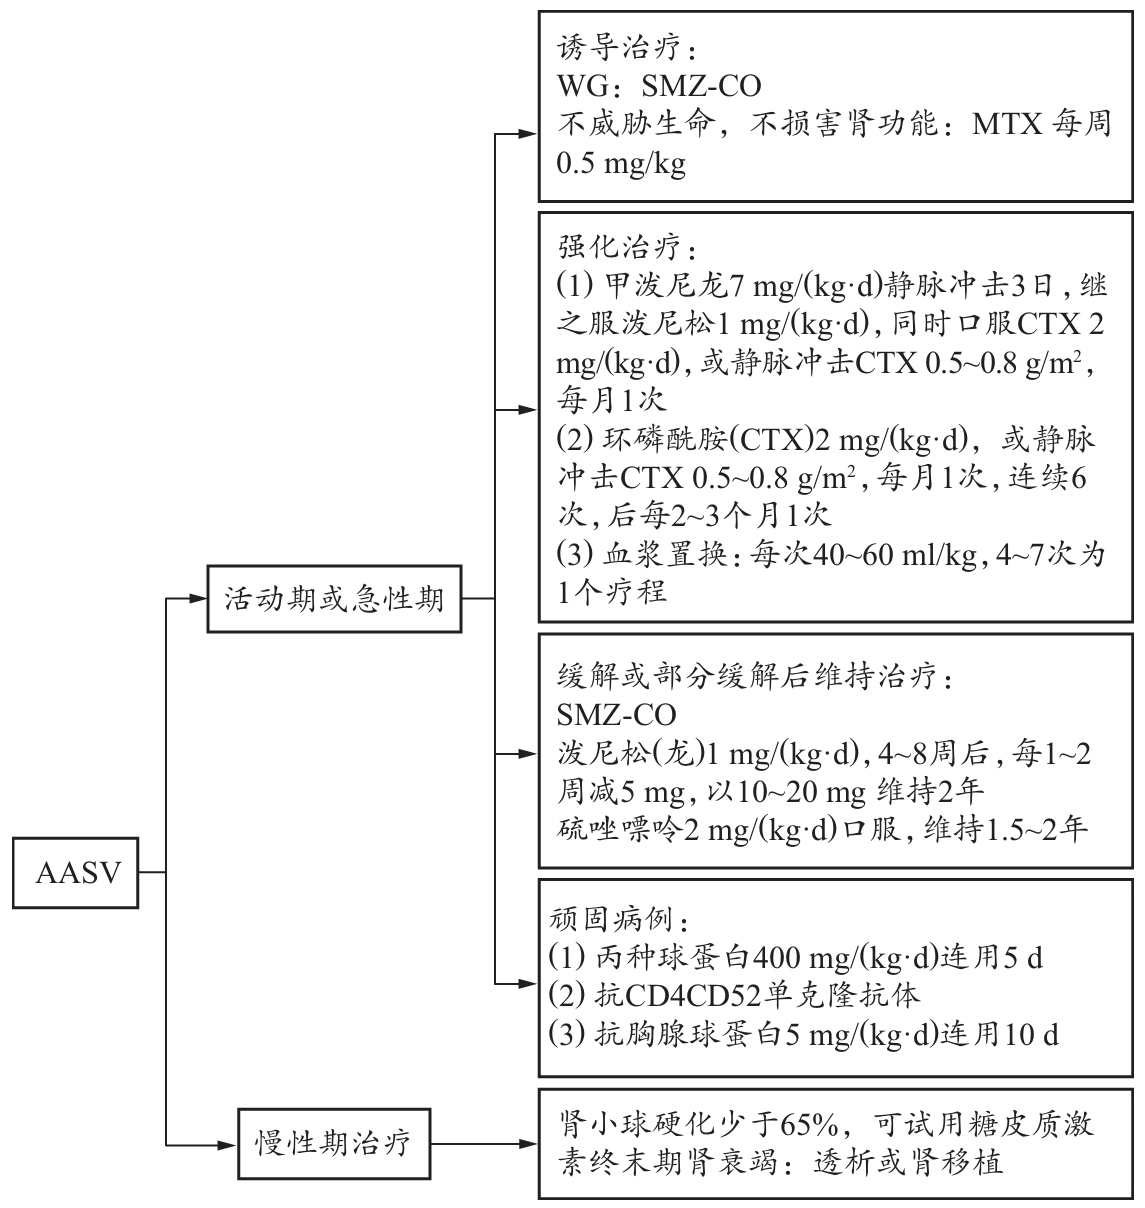
\includegraphics{./images/Image00127.jpg}
 \captionsetup{justification=centering}
 \caption{ANCA相关小血管炎(AASV)肾损害的治疗程序}
 \label{fig4-2-3}
  \end{figure} 

【治疗方案】 AASV的治疗方案分为诱导治疗、维持缓解治疗以及复发的治疗。诱导期的治疗主要是应用糖皮质激素联合细胞毒性药物,对于重症患者应采取必要的抢救措施,包括大剂量甲基泼尼松龙(MP)冲击和血浆置换;维持缓解期主要是长期应用免疫抑制药物伴或不伴小剂量糖皮质激素治疗。

1.
一般治疗 ①去除病因,如避免或消除药物过敏原,对病因进行治疗如抗感染等。感染可能是原发性小血管炎复发和(或)发病的诱因,尤其是肉芽肿性多血管炎。鼻部携带金黄色葡萄球菌是肉芽肿性多血管炎复发的重要原因,应用复方新诺明可明显减少复发。②治疗基础疾病,如结缔组织病,肿瘤等。

2. 药物治疗

(1)诱导期的治疗:糖皮质激素联合细胞毒药物,特别是环磷酰胺(CTX)可明显提高患者生存率。目前糖皮质激素联合环磷酰胺仍为治疗AASV特别是伴有肾脏损害的首选方法,能够使90\%以上的患者临床显著缓解,其中完全缓解率约为75\%。泼尼松(龙)初期治疗为1mg/(kg·d),4\textasciitilde{}8周,病情控制后可逐步减量,治疗6个月可减至10\textasciitilde{}20mg/d。糖皮质激素治疗的时间一般为1.5\textasciitilde{}2.0年。对于重要脏器受损的重症患者,如存在小血管纤维素样坏死、细胞新月体和肺出血的患者,可采用甲基泼尼松龙冲击疗法来尽快控制病情。一般为每次0.5\textasciitilde{}1.0g,每日1次,3次为1个疗程,继以口服泼尼松(龙)治疗。

环磷酰胺静脉冲击疗法在国内得到广泛应用。常用方法为0.75g/m{2}
(多为0.6\textasciitilde{}1.0g),每月1次,连续6个月。环磷酰胺口服剂量为1\textasciitilde{}3mg/(kg·d),一般选用2mg/(kg·d),分2次服用;持续3\textasciitilde{}6个月。

病情不重或对CTX禁忌者可选用利妥昔单抗及糖皮质激素作为初始替代治疗。

(2)维持期的治疗:常用的维持缓解治疗是小剂量糖皮质激素联合免疫抑制剂。AASV患者完全停药后易于复发,因此目前倾向于维持缓解治疗至少18个月。常用的维持治疗的药物:①环磷酰胺:在完成诱导缓解的基础上,每次静脉点滴环磷酰胺0.6\textasciitilde{}1.0g,2\textasciitilde{}3个月一次,总疗程1.5\textasciitilde{}2.0年。②硫唑嘌呤:在维持缓解治疗阶段,硫唑嘌呤是替代环磷酰胺证据最强的药物。常用剂量为1\textasciitilde{}2mg/(kg·d)。③吗替麦考酚酯:作为一种新型的免疫抑制剂,已有应用其成功治疗难治性小血管炎的报道。但其长期应用的疗效和安全性还有待于进一步的研究证实。常用剂量每日1.0\textasciitilde{}2g,分2次。④来氟米特:已有人应用来氟米特作为维持缓解治疗的药物成功用于WG。但关于来氟米特治疗AASV的疗效和长期安全性还有待进一步研究。常用剂量每日20mg维持。

(3)复发的治疗:尚缺乏循证医学证据。在病情出现小的波动时,可以适当增加糖皮质激素和免疫抑制剂的剂量;而病情出现大的反复时,则需要重新开始诱导缓解治疗。

(4)血浆置换:主要适应证为合并抗GBM抗体、严重肺出血或重症急性肾衰竭。每次置换血浆2\textasciitilde{}4L,每日1次,连续7日,其后可隔日或数日1次,至肺出血或其他明显活动指标如高滴度ANCA等得到控制。

【疗效观察与随访】

1.
观察指标 连续监测ANCA的滴度、临床表现以及炎症活动指标(如C-反应蛋白与血沉),调整治疗方案。

2.
疗效评估 诱导缓解后的复发率高达25\%以上;远期肾存活率低,5年肾存活率不足75\%。治疗目标力争达到临床缓解,提高存活率。

3.
随访 密切观察病情变化,定期复查C-反应蛋白、血沉等指标,连续监测ANCA滴度,随时调整治疗方案。

【治疗经验与解析】

1. 若为继发性小血管炎,需治疗原发病。

2. 如果存在肾脏损害,应积极行肾活检,根据病理确定治疗方案。

3.
使用糖皮质激素及免疫抑制剂时,应监测血常规、肝肾功能情况。如果发生感染,应积极抗感染治疗。

4.
10\%\textasciitilde{}20\%原发性小血管炎患者进入ESRD,而依赖维持血液透析治疗。

\subsection{骨髓瘤肾病}

多发性骨髓瘤(MM)是一种恶性浆细胞克隆性增生疾病。以骨髓内有恶性浆细胞(骨髓瘤细胞)的增殖与聚集,并分泌单克隆免疫球蛋白(M蛋白)为特征。主要表现为贫血、出血、溶骨性损害、病理性骨折、高钙血症、肾功能损害。发病高峰50\textasciitilde{}65岁,男女比约为2∶1。MM国内诊断标准:①骨髓浆细胞增多\textgreater{}15\%,有异常浆细胞或组织活检为浆细胞瘤。②血中大量M蛋白:IgG\textgreater{}35g/L,IgA\textgreater{}20g/L,IgM\textgreater{}15g/L,IgD\textgreater{}2g/L,IgE\textgreater{}2g/L,或尿中本周蛋白\textgreater{}1g/24h。③无其他原因的溶骨性病变或广泛骨质疏松。骨髓瘤性肾病是MM最常见和严重的并发症,又被称为骨髓瘤管型肾病(CN)。由于大量轻链从肾脏排泄,加之高血钙、高尿酸、高粘滞综合征等因素,就诊时50\%以上患者已存在肾功能不全。其肾脏受累可表现为蛋白尿,肾小管功能不全,肾病综合征,慢性肾衰竭及急性肾衰竭。

【治疗方案】 对无症状、无骨损害、无进展证据的冒烟型MM或ⅠA期患者可暂不治疗,每3\textasciitilde{}6个月随访检查1次,每年1次骨骼平扫,至病情进展、出现症状时开始治疗。当患者出现血、尿中M蛋白进行性增加、贫血、高钙血症、肾功能不全、骨痛、溶骨性损害、病理性骨折以及髓外浆细胞瘤等症状时开始治疗。

1.
一般治疗 加强隔离,口腔、外阴护理;感染时加强抗感染治疗,可静滴丙种球蛋白等支持治疗;贫血时促红细胞生成素治疗,重度贫血时输红细胞悬液纠正;并发粒细胞缺乏时可用粒细胞巨噬细胞集落刺激因子(GM-CSF)治疗。

2. 骨髓瘤的治疗 见血液病相关章节。

3. 肾脏损害的治疗

(1)去除加重肾损害的因素:预防肾衰竭很重要,去除引起肾功能不全的诱因,如脱水、高尿酸血症、高钙血症、感染尤其是尿路感染;避免使用一切肾毒性药物,如氨基糖苷类、非甾体类抗炎药和造影剂等。

(2)充分水化:除心衰和重度水潴留外,患者应充分水化,保证尿量\textgreater{}2\textasciitilde{}3L/d,以利于轻链、钙、尿酸和其他有害代谢物的排泄,减少肾小管和集合管内管型形成。

(3)碱化尿液:减少尿酸和轻链在肾内沉积,可口服和静脉注射碳酸氢盐,维持尿pH在6.5\textasciitilde{}7之间。

(4)防治高尿酸血症:口服别嘌呤醇0.05\textasciitilde{}0.3g,每日3次(根据肾功能调整)。

(5)防治高钙血症:骨髓瘤中发生有症状的或无症状的高钙血症的患者达到30\%。轻度高钙血症(血钙\textless{}3.0mmol/L)无症状,不需紧急处理,但需预防脱水,予以水化,避免使用肾毒性药物;中度高钙血症(血钙3.0\textasciitilde{}3.5mmol/L),视症状轻重予以正确处理;重度高钙血症(血钙\textgreater{}3.5mmol/L),可迅速导致脱水、肾衰竭及多器官受损表现。需紧急处理:①水化利尿:严重高钙血症常有多尿、脱水,甚至微循环衰竭,首先必须立即补液纠正脱水。补液量视脱水程度和心功能情况而定,一般每日补液3000ml\textasciitilde{}4000ml,应首先补给等渗盐水,肾脏排钠增加的同时也增加钙的排出。脱水一旦纠正,可适当应用利尿剂。可静脉推注呋塞米(速尿)40\textasciitilde{}80mg,必要时2\textasciitilde{}6小时后重复1次,注意监测电解质;但不能用双氢克尿噻,此药在抑制Na{+}
、Cl{-} 重吸收时也增加了K{+} 、Mg{2+} 的排泄而减少Ca{2+}
和尿酸的排泄。②糖皮质激素:口服泼尼松40\textasciitilde{}60mg/(m{2}
·d)或静脉用甲泼尼龙或地塞米松,可通过减少钙从肠道吸收,增加尿钙排出,抑制破骨细胞活性和对肿瘤细胞的直接作用而迅速降低血钙和改善脑病。③双磷酸盐类药物:如果血清肌酐\textgreater{}265μmol/L,建议不使用。④降钙素抑制骨重吸收和增加肾脏钙的排泄,皮下注射或肌内注射4U/kg,12小时1次,其作用较弱,常与激素合用。⑤化疗:初治或复发MM患者,在处理高钙的同时应尽早化疗。

(6)血液净化治疗:

1)透析:适用于严重肾衰竭患者,并可治疗高钙危象。长期血液透析已成为MM合并终末期CRF的维持性治疗手段,早期透析可减少尿毒症并发症和避免大剂量糖皮质激素引起的高代谢状态。透析同时给予适量剂量的化疗,亦可取得较满意的疗效,进一步延长其生存期。应仔细监测患者残余肾功能,部分患者有可能透析数月后肾功能改善而脱离透析。美国骨髓瘤透析患者1年存活率为54\%。老年患者心血管并发症较多,血液透析时应避免过分超滤液体,加重高粘滞血症;同时可适当灌注碳酸氢钠,促进管型和轻链的排出。腹膜透析对清除游离轻链可能较血液透析为好,但易并发感染。

2)血浆置换:目前主要用于治疗高粘滞综合征及MM相关的快速进展肾衰,方案多在10\textasciitilde{}14日内行6次单膜或双膜血浆置换,注意血浆置换与使用化疗药物应相隔一定时间。

(7)肾脏移植:肾脏移植只适用于很少数严格选择的患者(MM治疗有效,预后良好)。尚无充分循证医学证据支持终末期MM患者行肾移植治疗。

【疗效观察与随访】

1.
观察指标 常见症状与体征、骨髓常规、免疫球蛋白或M蛋白定量、肾功能、血钙等。

2.
疗效判断 完全缓解(CR),是指血、尿免疫固定电泳单克隆带消失及骨髓浆细胞\textless{}5\%;几乎完全缓解(nCR),是指单克隆带在常规血清蛋白电泳中不显示,仅在免疫固定电泳中显示。有报道这两者5年生存率分别为72\%、35\%。部分缓解或无反应者预后更差。

3.
随访 在治疗过程中至少每隔3个月进行1次免疫球蛋白或M蛋白定量,定期检测血常规、肾功能及血钙,每年进行骨髓常规检查及症状评估,视临床需要进行骨髓活检,并考虑PET/CT或MRI。

【治疗经验与解析】

1.
双磷酸盐类药物的常见的副作用包括感冒样症状、胃肠道症状(主要是口服制剂)、眼部不良反应、颌骨坏死、贫血、肾功能异常。根据肾功能情况调整药物用量。

2.
化疗时,为防止肿瘤细胞溶解综合征发生,充分水化、碱化尿液,并利用利尿剂及别嘌醇等辅助治疗。监测肾功能,严重肾功能不全应考虑血浆置换,必要时可血液透析或腹膜透析。

\section{肾小管间质性肾炎}

\subsection{急性间质性肾炎}

急性间质性肾炎(AIN)是指各种原因引起的肾小管和间质的病变,常见肾小管上皮细胞水肿、变性、坏死,间质细胞浸润等,常见于药物过敏性、感染相关性及特发性等因素。

急性过敏性间质性肾炎为双侧性非化脓性肾间质性病变,肾间质病变以淋巴细胞、单核细胞伴有嗜酸性粒细胞浸润为特征,肾小管常出现退行性变甚至坏死。细菌感染所致急性间质性肾炎,有两种形式:一种是细菌直接侵犯肾盂及肾实质所致的化脓性炎症;另一种是全身性或肾外感染引起的急性间质性肾炎,并非细菌直接侵犯肾间质,而是细菌或毒素的免疫反应。特发性急性间质性肾炎的肾组织学特点为典型的急性肾间质性肾炎,而无特异性的病因,临床以非少尿型急性肾衰竭为突出表现。常伴发眼色素膜炎,故又称“肾小管-间质性肾衰竭-眼色素膜炎”。三者的共同病理改变包括肾小管上皮细胞变性、坏死和间质炎细胞浸润等。

【治疗方案】

1.
对症支持治疗 注意休息,限制活动,充分的支持治疗,包括维持水、电解质和酸碱平衡,注意调节血容量以保证足够的尿量,同时避免水负荷过多。如有肾功能异常,尿量减少应适当限盐限水。提供足够热量25\textasciitilde{}30kcal/kg。慎用肾毒性药物。

2.
病因治疗 ①对于过敏性AIN,应尽可能去除过敏因素和诱发因素,停用致病药物或可疑致病药物,避免再次使用同类药物。如多重用药难以明确何种药物致病,应尽量减少用药种类,并尽快根据临床表现分析出何种药物,并停药观察。②对于感染引起的AIN,根据药敏试验选取敏感抗生素,积极控制感染,感染不是很重,可首选口服抗生素,一般为2周,如重症感染,应静脉抗感染治疗,如感染控制理想,3日后改为口服抗生素。如病情较重,感染控制不佳,可持续静脉使用抗菌药物,完成2周疗程。③对于特发性AIN,原因一般不清,应去除或避免能加重损害的因素或者其他加重肾脏负荷的因素,避免过敏和感染等因素。

3.
药物治疗 ①大剂量补充维生素C、维生素E,静脉使用古拉定,这些药物可以抗氧化,减少氧自由基的产生。②对明确为药物相关性AIN或诊断为特发性AIN,激素使用的指征为肾功能急剧下降、肾活检有弥漫肾损害及需要透析治疗的患者,可合理使用糖皮质激素,一般泼尼松30\textasciitilde{}60mg/d,根据恢复情况逐渐减量,对于急性重症者,可先用甲泼尼龙0.2\textasciitilde{}0.5g,静脉滴注,连续使用3日后序贯改服泼尼松或口服甲泼尼龙。对肾功能损害较轻和停用致病药物就能增加肾小球滤过率的患者则可不用激素。另外,一般认为感染相关性AIN只需积极控制感染即可,但也有学者建议在有效控制感染或者感染控制同时病情未见好转者可适当使用小剂量糖皮质激素,临床观察发现短期使用有助于改善预后。糖皮质激素的总疗程2\textasciitilde{}4个月,若2周内仍无好转,可加用环磷酰胺,1\textasciitilde{}2mg/(kg·d)。如用环磷酰胺治疗5\textasciitilde{}6周肾功能无改善者,则停药;如果肾小球滤过率有改善则继续用环磷酰胺1\textasciitilde{}2个月,并逐渐减少糖皮质激素,以及随之减少环磷酰胺用量。治疗时细胞毒药物时间不宜过长,防止用药后的并发症。在用环磷酰胺治疗同时,应充分水化碱化。其他的免疫抑制剂如骁悉等近来也有临床应用。③另外,也可用一些活血化瘀药物和百令胶囊,以及中医中药治疗,以促进肾间质小管细胞的恢复。

4.
替代治疗 掌握肾替代治疗时机的选择,一般急性间质性肾炎较少有尿量减少,如无明显尿量减少,无明显酸中毒及电解质紊乱,可暂不血透,药物治疗为主,但如保守治疗欠佳,应尽快开始透析;如出现明显少尿或者无尿,有严重的电解质紊乱和严重酸中毒,或血Cr≥8\textasciitilde{}10mg/d时应尽量在并发症发生之前开始透析。一般情况下,在停用致病的相关药物,经积极地对症支持治疗后,药物相关性AIN通常可脱离透析并逐渐恢复。而中药所致肾损害,尽管已停用中药,肾功能衰竭仍进行性发展,而且近半数患者需做肾功能替代治疗。

【疗效观察与随访】

1.
观察指标 主要观察尿量、血常规、尿常规、肝肾功能、电解质、尿酸、血清蛋白电泳,血、尿免疫固定电泳、血、尿NAG酶,血清血、尿中β{2}
-微球蛋白,尿比重、尿渗透压,尿浓缩稀释功能障碍,肾脏超声等。

2.
疗效观察 一般来说,药物相关性AIN,在及时发现并停用致病药物后经积极治疗,在6周到1年内小管功能可恢复,但也有40\%的患者因诊断延误、停药不及时,以及治疗过程中再次使用同类或其他致病药物而加重病变,使急性间质性肾炎慢性化,部分甚至进入终末期肾衰竭。AIN预后不良的因素包括:①血肌酐水平持续\textgreater{}3mg/ml或者急性肾衰竭持续时间过长,有研究证实,急性肾衰竭持续3周以上的急性AIN,其预后显著差于持续两周以内的患者。②肾间质炎症细胞浸润的范围弥漫和程度重,有肉芽肿形成。③肾间质病变累及肾小球或肾小管,肾小管萎缩或者间质纤维化严重。④致病药物的种类也可能会影响预后。

3. 随访 密切观察病情变化,定期复查尿常规、肝肾功能及免疫指标的检测。

【治疗经验与解析】

1.
药物相关性AIN,应尽早根据临床表现及用药经过来判断出致病药物,及时停止使用致病药物有利于疾病恢复。感染相关性AIN,需根据药敏选择合适的抗生素治疗,才能更好更快地控制感染,消除病因。

2.
AIN患者应给予足够的营养支持,以利于肾间质小管的能量摄取和自我修复。如患者出现尿量减少,血压升高,适当限盐限水,有利于减轻体内容量负荷,减轻肾脏负担,从而减少并发症,并有利于肾脏的恢复。

3.
药物相关性AIN和特发性AIN,在去除病因后如疾病恢复不理想、进一步发展,或病理提示弥漫炎细胞浸润等,应及时使用糖皮质激素,感染相关性AIN在有效抗感染同时也主张小剂量使用糖皮质激素。并密切观察两周内激素治疗效果,如不理想,应尽早联合使用细胞毒药物。如病理上已有明显的间质纤维化、小管萎缩或坏死时均不主张再使用免疫抑制剂治疗。

4.
对于AIN患者,如出现明显的水电解质及酸碱紊乱,或者少尿无尿严重,肌酐和尿素氮上升速度过快,建议及早行肾替代治疗。

5.
AIN的三种不同类型经及时明确诊断,尽早去除病因、合理治疗,一般预后良好,极少数进展至终末期肾衰竭。

\subsection{慢性间质性肾炎}

慢性肾小管间质性肾炎(CTIN),简称慢性间质性肾炎(CIN),是一组由多种病因引起的慢性肾小管间质疾病,临床以肾小管功能障碍为主,表现为尿浓缩功能障碍、肾小管酸中毒或Fanconi综合征、低钾血症等,晚期表现为慢性肾功能不全。可由急性间质性肾炎演变而来,也可无急性炎症过程。病理表现以肾间质纤维化、间质单核细胞浸润和肾小管萎缩为主要特征,起病初期可无肾小球和血管受累,晚期则有不同程度肾小球硬化。慢性间质性肾炎病因具有多样性,常见的有药物相关性CIN,如解热镇痛药、中草药、碳酸锂等,还有免疫相关性CIN,如系统性红斑狼疮,干燥综合征等,另外,代谢相关性CIN临床也较多见,如痛风性肾病,低钾性肾病等,不同的病因其临床表现也各不相同。以下主要就药物相关性CIN简单介绍一下其治疗方案。

【治疗方案】

1.
去除病因 服用解热镇痛药及含有马兜铃酸的植物、中草药及排石冲剂引起的慢性间质性肾炎重在早诊断早停药早治疗,避免其他潜在或反复存在的损害因素。

2.
对症支持治疗 注意休息,避免过累,加强营养,维持水电解质平衡,保持尿量在1000\textasciitilde{}1500ml,纠正酸碱紊乱,低钾本身也会加重间质损害,应及时纠正;如合并有感染,应根据药敏,选用肾毒性小的抗生素,积极控制感染;对有血压升高者,应严格控制血压,一般不主张使用利尿剂来控制血压,首选ACEI或ARB。如血压控制不理想可联合其他药物治疗,也有部分学者认为使用小剂量糖皮质激素有利于肾功能的恢复。对于有慢性肾功能不全的患者,应予优质蛋白饮食,开同补充必须氨基酸。出现贫血,可使用促红细胞生成素(益比奥等)、叶酸、铁剂等纠正贫血。对于严重肾功能不全时的钙和磷代谢异常也需积极纠正。

3.
药物治疗 主要对于原发性疾病而言,特别是免疫相关性CIN,原发病治疗尤为重要,系统红斑狼疮应首先控制狼疮活动,根据肾活检病理和临床表现明确分期,选用糖皮质激素和(或)免疫抑制剂治疗;干燥综合征也可合并肾小管酸中毒或肾性尿崩症,补充碱剂纠正酸中毒及合理对症处理,均有利于保护肾脏,延缓其进展。

4.
肾替代治疗 慢性间质性肾炎临床可表现为慢性肾衰竭急性进展,这就需要及时行肾替代治疗。对于缓慢发展至终末期的CIN,根据内生肌酐清除率的监测决定肾替代治疗的时机。

【疗效观察与随访】

1.
观察指标 尿量、血常规、尿常规、肝肾功能、电解质、尿酸、血、尿NAG酶,尿β{2}
-微球蛋白,尿渗透压,尿酸化功能,内生肌酐清除率,血气分析,肾脏超声等。

2. 疗效观察 显效:症状、体征消失,相关检测指标尚有部分未能完全恢复。

解热镇痛药肾病和马兜铃酸肾病,停药后轻症患者可能肾功能相对稳定或一定程度上有好转,但多数患者肾功能可持续进展,直至进入终末期肾衰竭需行肾替代治疗或移植。对于各种病因所致的慢性间质性肾炎,如出现肾功能损害、高血压、贫血等都提示预后不良。

3.
随访 密切观察病情变化,及时作出治疗评估,定期复查相关检测指标,指导出院后的保健。

【治疗经验与解析】

1.
对于患有慢性疼痛感、关节炎等疾病需要长期或反复使用药物人群,应监测小管间质功能,及时减药或停药,可避免或减轻药物对肾脏的损害。解热镇痛药肾病和马兜铃酸肾病的肾损害一般为非可逆的,目前没有好的治疗方法。

2.
慢性间质性肾炎,病理主要以慢性病变为主,因此一般不主张大剂量长期使用糖皮质激素和免疫抑制剂,只有在其存在急性加重因素或者病理提示存在大量炎细胞浸润时才考虑小剂量使用,时间不宜过长。在使用免疫抑制剂时更应警惕其肾损害的副作用。

\section{尿路感染}

\subsection{肾盂肾炎}

肾盂肾炎是泌尿系统感染性疾病,包括急性肾盂肾炎和慢性肾盂肾炎。急性肾盂肾炎是指肾盂粘膜及肾实质的急性感染性疾病,主要是大肠杆菌的感染,占80\%\textasciitilde{}85\%,另外还有变形杆菌、葡萄球菌、粪链球菌及绿脓杆菌等引起。在婴幼儿和儿童中,尿路感染的发病率占感染性疾病中的第二位。新生儿中,尿路感染在男性较女性更多见,常伴有菌血症,这与男婴泌尿道先天性异常较高发生率有关。因为泌尿生殖系统解剖的不同,其他年龄段女性发病率明显高于男性,\textgreater{}50岁后男性发病率有所增加,乃因前列腺疾病发生率增加之故。慢性肾盂肾炎是指尿路感染病史超过1年并有肾盂、肾盏粘膜和间质纤维化瘢痕变形,或经治疗后仍有肾小管功能减退者。完整意义上的慢性肾盂肾炎实际上由三种疾病组成:伴有反流的慢性肾盂肾炎(反流性肾病);伴有尿路梗阻的慢性肾盂肾炎(慢性梗阻性肾盂肾炎);特发性慢性肾盂肾炎。

【治疗方案】

1.
一般治疗 急性期有高热者应卧床休息,鼓励多饮水、勤排尿、促使细菌及炎性渗出物迅速排出。

2.
抗菌治疗 一般在无尿培养结果和药敏试验结果之前,首选对革兰阴性杆菌有效的药物,因尿路感染大多由大肠杆菌等革兰阴性菌引起,尤其是首发尿路感染,多数可以治愈。如治疗3日,症状无明显改善,则应根据药敏试验结果来更换抗菌药。急性肾盂肾炎抗菌药的疗程一般10\textasciitilde{}14日。慢性肾盂肾炎间隔5\textasciitilde{}7日后再进行下一疗程,直至尿常规及培养阴转时为止。常用的药物有氟喹诺酮类、β-内酰胺类、大环内脂类等,如左氧氟沙星0.3g,每日1次静脉滴注,头孢哌酮钠舒巴坦钠2.0g,每日2次静脉滴注。

3.
增加抗菌药疗效 可口服苏打等碱化尿液,增加喹诺酮类、氨基糖苷类抗菌药疗效。碳酸氢钠1.0g口服,每日3次。

4.
抑菌治疗 慢性肾盂肾炎在抗菌疗法无效时,可用抑菌疗法。具体方法:选用敏感抗生素,每晚睡前排空膀胱后服常规剂量的半量,连续3\textasciitilde{}6个月,期间可以是几种抗生素轮转服用,约60\%患者尿培养可阴转。此法费时长,应注意药物的毒副作用。

5.
病因治疗 对于有尿路梗阻及感染原因(如尿路结石、膀胱颈梗阻、盆腔感染等)者,应及时排除并针对病因治疗。

【疗效观察与随访】

1.
观察指标 治疗后观察尿频、尿急、尿痛、发热、腰痛等症状的改善情况。复查尿常规、血常规、尿培养等指标。

2.
治愈标准 疗程完毕后症状消失,尿常规、尿培养阴性,并于第2周、6周复查尿菌仍阴性。

3. 随访 注意治疗后的病情变化,定期复查相关指标,指导离院后保健。

【治疗经验与解析】

1.
急性肾盂肾炎一般用药72小时内即显效,如有效则不需要药敏结果换药,因为体内药敏试验最准确。如用药72小时仍未显效,应按药敏结果更换抗菌药物。

2.
重症肾盂肾炎在病情允许时,应尽快作有关尿路影像学检查,以确定有无尿路梗阻,如不纠正尿液引流不畅,复杂性肾盂肾炎很难彻底治愈。

3.
复杂性肾盂肾炎易于发生革兰阴性杆菌败血症,应联合使用两种或两种以上抗生素治疗。用药期间,应每1\textasciitilde{}2周复查尿细菌培养,以观察细菌是否转阴。经治疗仍持续发热,应注意肾盂肾炎并发症的可能,如肾盂积脓、肾周脓肿等。

4. 妊娠期肾盂肾炎应积极治疗,宜选用毒性小的抗菌药物,如青霉素或罗氏芬。

5.
慢性肾盂肾炎急性发作期治疗疗程需足够,避免因疗程不足致耐药菌产生导致反复发作。

\subsection{膀胱炎}

膀胱炎即通常所指的下尿路感染,是一种常见的尿路感染性疾病,占尿路感染总数的50\%\textasciitilde{}70\%,其致病菌多数为大肠杆菌。膀胱炎可分为急性与慢性两种,两者又可互相转化,急性膀胱炎得不到彻底治疗可迁延成慢性,慢性膀胱炎在机体抵抗力降低或局部病变因素加重时,又可急性发作。通常多发生于女性,因为女性的尿道比男性的尿道短,又接近肛门,大肠杆菌易侵入。男性若有尿路梗阻如前列腺肥大或膀胱结石、异物等也易患膀胱炎。

【治疗方案】

1.
一般治疗 急性膀胱炎患者需适当休息,多饮水以增加尿量,注意营养,忌食刺激性食物,热水坐浴可减轻症状。膀胱刺激症状明显的患者给予解痉药物缓解症状。此外,还应注意尿路卫生,尤其女性更应注意。

2.
抗感染治疗 根据尿细菌培养药敏结果选用有效的抗菌药物,如头孢呋辛0.5g,每日2次口服,或左氧氟沙星0.3g,每日1次静脉滴注。急性膀胱炎疗程3\textasciitilde{}7日,若症状不消失,尿脓细胞继续存在,细菌培养仍为阳性,应考虑细菌耐药或有感染诱因存在,要及时调整更适合的抗菌药物,延长应用时间以期达到早日治愈的目的。慢性膀胱炎疗程要长,10\textasciitilde{}14日,必要时采用抑菌治疗。

【疗效观察与随访】

1.
观察指标 治疗后观察尿频、尿急、尿痛等症状的改善情况。复查尿常规、尿培养等指标。

2.
治愈标准 治疗后症状消失,尿常规、尿培养阴性,并于第2、6周复查尿菌仍阴性。

3.
随访 注意观察治疗后的病情变化,必要时复查尿常规、中段尿培养。对慢性患者应加强卫生指导。

【治疗经验与解析】 对于久治不愈或反复发作的慢性膀胱炎,要做详细全面的泌尿系检查,包括膀胱镜检,找出病因后给予针对性治疗。同时要重视预防,对急性病例必须彻底治愈。

\subsection{无症状性菌尿}

无症状性菌尿又称隐匿型菌尿,是一种隐匿型尿路感染,即指患者有真性细菌尿而无任何尿路感染的症状,其细菌来自肾脏或来自膀胱。无症状性菌尿可以由症状性尿感演变而来,有些也可无急性尿感既往史,此外在尿路器械使用后发生的和在慢性肾脏病的基础上发生的尿感,常常无明显症状。无症状性细菌尿在16\textasciitilde{}65岁的女性中发病率均为4\%,男性为0.5\%。

【治疗方案】

1.
抗菌治疗 无症状性菌尿是否需要抗菌治疗,意见尚未完全统一,一般认为下列情况需要治疗:

(1)存在膀胱输尿管反流时:应给予治疗,因为膀胱输尿管反流时的菌尿多数为肾盂肾炎,此时极易产生肾实质损害和瘢痕,即所谓反流性肾病。

(2)孕妇伴无症状性菌尿:发病率为3\%\textasciitilde{}7\%,如果不治疗,25\%\textasciitilde{}40\%可发展成症状性尿路感染(常在第18\textasciitilde{}30周发生),早产儿和体重不足婴儿较无细菌尿的孕妇多见,其中20\%\textasciitilde{}40\%可并发败血症。因此,对有无症状性菌尿孕妇应立即治疗。

(3)伴有结石或梗阻的无症状性菌尿:应立即治疗,并去除结石或梗阻。大多数变形杆菌、部分葡萄球菌和粪链球菌的尿路感染常并发结石,这些细菌含有尿素分解酶,可使尿中的尿素分解,释放出氨,使pH值增高,结果使钙-铵-镁-磷酸盐沉淀,导致尿结石生成。结石形成后治疗就更困难,感染复发率高。

2. 手术治疗 无症状菌尿合并重度膀胱输尿管反流、结石或梗阻时需手术治疗。

【疗效观察与随访】

1.
观察指标 观察有无尿频、尿急、尿痛、发热、腰痛等症状的出现,若有,按有症状性菌尿治疗,并复查尿常规、尿培养等指标。

2.
治愈标准 若行抗菌治疗,治疗后复查尿常规、尿培养等均阴性,3个月内无复发。

3. 随访 治疗后3个月内每月复查尿常规、中段尿培养1次,密切观察病情变化。

【治疗经验与解析】 关于抗感染治疗无症状性菌尿后能显著改善预后的研究资料还非常有限。由于抗菌药物耐药性的增加,目前比较倾向于不治疗无症状性菌尿,除非获得患者能从中获益的证据。一旦出现相关症状,即应进行抗菌治疗。

\subsection{尿道综合征}

尿道综合征是指有下尿路刺激症状,无明显膀胱尿道器质性病变及菌尿的一组症候群,而非一种疾病。临床上常见,占膀胱刺激征的45\%\textasciitilde{}50\%,多发生于女性。

【治疗方案】

1.
药物治疗 可予药物调整膀胱、尿道功能失调,调整植物神经系统功能,增加膀胱逼尿肌的收缩。如谷维素10mg,口服每日3次,坦索罗辛0.2mg,口服每日1次。

2.
电刺激治疗 经皮胫神经刺激法,每周1次,每次30分钟,连续10周。其机制是控制膀胱功能的神经来自骶丛,其传入纤维为胫神经后部,刺激此处的神经能对膀胱起神经调节作用,可以治疗下尿道功能障碍引起的症状,包括尿频、尿急、尿失禁和盆腔疼痛。

3. 外科治疗

(1)尿道扩张:1\%丁卡因尿道粘膜浸润麻醉,将涂有石蜡油的尿管从尿道口插入,如插入困难可先用宫颈扩张器稍加扩张,导管持续牵引固定30分钟。解除尿道梗阻达到治疗目的。适应证:经久不愈者;远端尿道的肌肉痉挛;远端尿路旁纤维增生。并发症:尿失禁,尿道少量渗血。休息、多饮水、服用消炎药等多可止血。

(2)尿道松解术:尿道阴道隔远端1/2弹力组织是增加US的病因,通过手术去除尿道阴道膈间的组织索,然后反折阴道壁盖于尿道上重建阴道层。

(3)其他外科治疗方法:包括尿道冷冻术、去除Skene氏腺的梗阻等。

4. 心理及物理治疗 保持心情愉快,多参加社会活动,加强体质锻炼。

【疗效观察与随访】

1.
观察指标 治疗后观察尿频、尿急、尿痛等尿路刺激症改善情况,监测尿常规、尿培养等指标。

2. 治愈标准 尿频、尿急、尿痛等尿路刺激症好转。

3.
随访 治疗后密切观察病情变化,加强心理疏导,保持心情愉快至少坚持3\textasciitilde{}6个月。

【治疗经验与解析】 对病变应提高认识,避免误诊为尿路感染而长期用抗生素治疗,不但无效,反而会带来抗生素引起的一些不良反应,也给患者造成不必要的经济损失和精神痛苦。

\section{肾小管疾病}

\subsection{肾小管酸中毒}

肾小管酸中毒(RTA)是由于近端肾小管对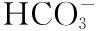
\includegraphics{./images/Image00128.jpg}
的再吸收障碍或远端肾小管泌氢功能障碍而使肾小管的血液和管腔间不能建立正常的pH梯度所引起的一组临床综合征。其临床特征为阴离子间隙(AG)正常的高血氯性代谢性酸中毒,水、电解质紊乱。可有低钾血症或高钾血症、低钙血症及多尿、多饮、肾性骨病、肾结石等。肾功能不全时的酸中毒同时包括肾小球和肾小管损伤所致的酸中毒,主要以小球性因素为主,因此我们常提到的RTA没有把这一部分包括在内。

肾小管酸中毒按病因分为原发性和继发性;按是否发生全身性代谢性酸中毒分为完全性和不完全性;按病变部位分为四型,远端型(Ⅰ型或者经典型)、近端型(Ⅱ型)、混合型(Ⅲ型)和高血钾型(Ⅳ型),这是临床最常用的分类标准。

【治疗方案】

1. Ⅰ型RTA治疗

(1)病因治疗:根据肾小管酸中毒的病因及时去除和治疗病因,慎用一些肾毒性药物,如非甾体类解热镇痛药,两性霉素B,磺胺类及乙酰唑胺等药物;一些自身免疫性疾病如干燥综合征、系统性红斑狼疮等及时有效的治疗;明确诊断一些遗传性系统性疾病,如Marfan综合征、镰状细胞性贫血等,及时选择合适方法进行治疗;避免感染,避免反复发生慢性肾盂肾炎,避免梗阻性肾病的长期不缓解。

(2)对症治疗:

1)纠正低血钾:对于一般血钾降低不是很严重患者,主张在明确诊断后口服补钾,如枸橼酸钾、枸橼酸合剂(枸橼酸100g+枸橼酸钾100g,稀释成1000ml溶液)或Albright合剂(每1000ml水中加入枸橼酸钾98g和枸橼酸140g),10\textasciitilde{}20ml,每日3次。如血钾降低很严重,有诱发恶性心律失常风险时,可静脉补充氯化钾,同时口服枸橼酸钾、枸橼酸合剂或者补达秀,待血钾有明显纠正后停止静脉补氯化钾。

2)纠正酸中毒:补充碱剂,一般常用口服碳酸氢盐或枸橼酸合剂,枸橼酸合剂除了补碱纠正酸中毒外还可以减少肾结石和钙化。酸中毒不很严重者可选用碳酸氢钠1.0g,每日3次口服,也可以用枸橼酸钠溶液(或者枸橼酸合剂)10\textasciitilde{}20ml口服,每日3次。对酸中毒严重者,可先静脉补充5\%碳酸氢钠100\textasciitilde{}200ml,然后序贯口服碱剂。对于儿童,补碱量要大,通常每日需5\textasciitilde{}14mmol/kg体重,可以减轻骨病的发生,防止生长发育迟缓。

3)纠正低钙等其他电解质紊乱及防止肾性骨病:患者除了低血钾外一般还有明显的低血钙、低血镁等电解质紊乱,因此根据实际水平予以口服或者静脉补充,一般情况下严重低钙时,在纠酸补钾后可谨慎使用钙剂和活性维生素D{3}
治疗。钙剂临床有葡萄糖酸钙1.0g,每日3次;碳酸钙1.0g,每日3次;维生素D{3}
临床有钙尔奇D0.6g,每日1次,骨化三醇(罗盖全)0.25μg,每日2次或3次。

2.
Ⅱ型RTA治疗 在能找到病因的以治疗病因为主,其他治疗基本类似于Ⅰ型RTA的治疗。部分Ⅱ型有自愈倾向,一般为2年。只是对于Ⅱ型RTA来说,酸中毒一般比较严重,补碱量要大(6\textasciitilde{}12g/d),对于重症Ⅱ型RTA,加用氢氯噻嗪25mg口服,每日3次,可促进肾小管对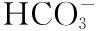
\includegraphics{./images/Image00128.jpg}
的重吸收。

3.
Ⅲ型RTA治疗 Ⅲ型RTA是Ⅰ型和Ⅱ型的混合型,需根据具体情况选择方案,基本以对Ⅰ型和Ⅱ型RTA的处理为参照。

4.
Ⅳ型RTA治疗 Ⅳ型RTA病因复杂,确诊有难度,氟氢可的松替代治疗对肾上腺功能不全或低肾素性低醛固酮血症有确切疗效,可试用氟氢可的松0.1mg/d,如果考虑系对醛固酮反应弱的病例,可加大剂量至0.3\textasciitilde{}0.5mg/d。噻嗪类利尿剂可抑制氯的吸收,可缓解水电解质紊乱程度,并改善容量负荷过重。血钾升高应及时有效处理,口服交换树脂或用排钾利尿剂,监测血钾水平,如大于6.5mmol/L或心电图有明显异常时及时安排透析治疗。其他纠正酸中毒和维持水电解质平衡同其他类型RTA。

【疗效观察与随访】

1.
观察指标 治疗观察尿量、夜尿量和次数,血常规,尿常规,尿酸化功能,尿渗透压,尿电解质排泄量,β{2}
-微球蛋白,肝肾功能,电解质,血气分析,甲状旁腺激素,血肾素、醛固酮水平,泌尿系B超检查。

2.
疗效评价 显效:没有明显酸中毒,无水钠潴留,无明显电解质紊乱,甲状旁腺激素水平正常范围,儿童生成发育及智力水平正常,无泌尿系结石或已有的泌尿系结石无明显增大增多,基础疾病实验室检查提示该疾病稳定,处于非活动期等。

3. 随访 密切观察病情变化,定期检测相关指标,如血尿常规,β{2}
-微球蛋白、肝肾功能、尿酸化功能、电解质、泌尿系B超检查等,随访应在6个月以上。

【治疗经验与解析】

1.
在补钾纠酸时,应先补钾再行纠酸,不然在纠酸后血钾会进一步下降而诱发恶性心律失常。仅在严重缺钾时可选用10\%氯化钾缓慢静脉滴注,但须监测血钾变化,及时过渡到口服补钾。同时氯化钾中有氯,甚至可加重酸中毒,在不是严重缺钾的危重情况下一般不主张。在服用碳酸氢钠、枸橼酸钠溶液、枸橼酸钾、枸橼酸合剂等时应监测血气分析和血钾。

2.
临床表现为近端肾小管酸中毒又合并肾性氨基酸尿、肾性葡萄糖尿、肾性有机酸尿、肾小管性蛋白尿、尿磷酸盐及电解质丢失等又称为范可尼综合征,由此引起低磷血症、低钙血症、脱水、骨质疏松等。

3.
肾小管酸中毒症状复杂多样,且缺乏特异性,可表现为厌食、恶心呕吐、腹泻、多饮多尿、佝偻病、骨折、生长发育落后等,且常继发于许多疾病如肝豆状核变性、先天性肾畸形等,易被误诊、漏诊。

4.
儿童Ⅰ型RTA常出现骨质软化,骨骼严重畸形、发育不佳,牙齿早脱等,维生素D治疗效果不佳,需终身用药,而Ⅱ型有自愈倾向,一般为两年。应用钙剂和维生素D时应慎防高钙血症和维生素D中毒,已有肾钙化者慎用。

5.
对于肾小管酸中毒,特别Ⅰ型患者应终身服药,不得间断。并定期复查尿常规,血气分析,电解质等,了解疾病的情况,以指导用药量调整和观察用药疗效,因此对此类患者建议最少随访6个月至1年。

6.
对已发生肾小管酸中毒患者,应避免加重因素,条件许可应终身禁用呋喃坦啶、磺胺药及乙酰唑胺等药物,因这些药物可加剧酸中毒,磺胺药及乙酰唑胺还能增加尿钙的排泄及对碳酸酐酶有抑制作用。

\subsection{Fanconi综合征}

Fanconi综合征是指由于近端肾小管转运功能缺陷,导致由该段肾单位处理的多种溶质重吸收障碍和排出过多,尤其是尿中葡萄糖、氨基酸、磷酸盐及尿酸丢失过多,这种小管重吸收功能的缺陷称为Lignac-de
Toni-Debre-Fanconi综合征,简称Fanconi综合征。还有许多其他物质的丢失,如小分子蛋白、激素、肽类物质、结合蛋白及碳酸氢盐等。其中碳酸氢盐的过多丢失可引起高氯性肾小管酸中毒,及近端肾小管酸中毒。

Fanconi综合征可见于先天性或遗传性疾病,也可见于后天获得性即继发性,由其他遗传性疾病或非遗传性疾病引起。根据临床表现的严重程度,可将其分为完全性和非完全性Fanconi综合征。Fanconi综合征患者多有钙、磷和维生素D代谢异常,可导致继发性维生素D抵抗性骨病,包括成人骨软化症和儿童佝偻病。

【治疗方案】

1. 继发性Fanconi综合征治疗

(1)病因治疗:如为外源性药物、毒物引起的,应尽快停用或减量药物,避免接触毒性药物;继发于自身免疫性疾病,骨髓瘤等血液性疾病,肿瘤,及慢性间质性肾炎,应积极治疗原发病,控制疾病活动。

(2)对症治疗:

1)纠正酸中毒:补充碱剂,酸中毒一般比较严重,补碱量要大(6\textasciitilde{}12g/d),碳酸氢钠2.0g,每日3次口服,也可以用枸橼酸钠溶液20\textasciitilde{}40ml口服,每日3次。对酸中毒严重者,也可先静脉补充5\%碳酸氢钠100\textasciitilde{}200ml,好转后改口服碱剂。重症Ⅱ型RTA也可加用氢氯噻嗪25mg口服,每日3次,可促进肾小管对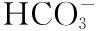
\includegraphics{./images/Image00128.jpg}
的重吸收。合并Ⅰ型RTA者,可给予枸橼酸合剂,如出现肾功能不全,改用碳酸氢钠为好。

2)纠正其他电解质紊乱:如有低钾血症、低镁血症或低磷血症,应予以相应补充,对于一般血钾降低不是很严重患者,口服补钾,枸橼酸钾、枸橼酸合剂(枸橼酸100g+枸橼酸钾100g,稀释成1000ml溶液)10\textasciitilde{}20ml,每日3次。如血钾降低很严重,有诱发恶性心律失常风险时,可静脉补充氯化钾,同时口服枸橼酸钾、枸橼酸合剂或者补达秀,待血钾有明显纠正后停止静脉补氯化钾。

3)防止肾性骨病:补充维生素D和钙剂,钙剂以碳酸钙为主1.0g,每日3次;也可用葡萄糖酸钙1.0g,每日3次;维生素D{3}
临床有钙尔奇D0.6g,每日1次,骨化三醇0.25μg,每日2次或3次。

2.
遗传性Fanconi综合征治疗 半乳糖血症治疗主要为无半乳糖饮食;遗传性果糖不耐受治疗包括严格限制果糖和蔗糖饮食;胱氨酸贮积症给予半胱胺,降低白细胞内胱氨酸浓度;Wilson病治疗药物有D-青霉胺,1g/d,可逆转肾损害。纠正酸中毒和水电解质紊乱,防治肾性骨病同继发性。

3. 终末期肾病治疗 可行肾替代治疗,血液透析和腹膜透析,也可行肾移植术。

【疗效观察与随访】

1.
观察指标 血常规,尿常规,尿NAG酶,尿酸化功能,尿渗透压,血气分析,肝肾功能、电解质,葡萄糖氧化试验,白细胞或直肠活检,肝活检测定醛缩酶水平,血浆铜蓝蛋白检测,肾活检等。

2.
疗效评估 一般预后很差,对症治疗只能暂时缓解症状、肾移植适用于终末期。

3. 随访 密切观察病情变化,加强医患沟通。

【治疗经验与解析】

1.
遗传性Fanconi综合征一般无根治方法,以对症处理为主,且预后不佳,最终进展至肾衰竭,需行肾透析治疗或肾移植,但有部分病例,如胱氨酸贮积症,也可在移植后复发。

2.
继发性Fanconi综合征,特别是毒物或药物所致者,一般早期只有肾小管和间质病变,小动脉和小球无病变或病变较轻。但从治疗观察情况而言,这些患者有一定可逆性,早期用一些糖皮质激素,在一定时间内肾功能可能会好转或稳定,各种临床表现也可能减轻。

3.
Fanconi综合征,特别是遗传性,多可能出现肝肿大、肝损害的表现,因此治疗时需注意保护肝脏,慎用对肝损害较大的药物。

\subsection{肾性糖尿}

在正常人,近端肾小管几乎重吸收肾小囊原尿中的全部葡萄糖,尿中只含及其微量的葡萄糖,一般常规检查不能检出,尿糖定性为阴性。但在肾小管疾病或者血糖浓度增加的情况下,超过肾小管摄糖阈值,尿中即开始排出较多的葡萄糖,这就是肾性糖尿。肾性糖尿主要分原发性和继发性肾性糖尿两类,原发性肾性糖尿,也称单纯性肾性糖尿,是一种肾小管吸收功能障碍的遗传性疾病,一般无其他肾小管功能障碍,肾小球滤过功能和小肠吸收功能也正常。原发性肾性糖尿至少有三种亚型:A型肾性糖尿,表现为肾糖阈下降,肾小管葡萄糖最大重吸收率(TmG)也下降,患者血糖水平正常,但有大量尿糖;B型肾性糖尿,表现为肾糖阈下降,TmG正常。一般血糖正常,也可合并有氨基酸尿或磷酸盐尿;O型肾性糖尿,在任何情况下均不能重吸收葡萄糖,大量尿糖,机制不清。继发性肾性糖尿,也称获得性肾性糖尿,引起这类肾性糖尿的因素较多,包括感染(如肾盂肾炎),药物性(马兜铃酸肾病),以及一些免疫性疾病累及肾小管等。

【治疗方案】 原发性肾性糖尿常是良性病变,常为体检发现,一般无需治疗,应避免饥饿,尤其对于严重糖尿患者和孕妇,避免出现低血糖,如出现低血糖症状应及时处理;继发性肾性糖尿主要是寻找原发疾病,及时去除或治疗病因。合并症具体治疗方法和用药参照Fanconi综合征的治疗。

【疗效观察与随访】

1.
观察指标 尿常规、血常规、尿NAG酶、肝肾功能、FBG、电解质、尿酸化功能、尿渗透压、HbA1C、TmG等。

2. 疗效评估 治愈标准:糖尿消失,症状消除,3个月内无复发。

3.
随访 定期监测尿常规、肾功能、血糖、尿糖水平,注意低血糖发生,原发疾病监测其肝肾功能、尿常规及活动指标,控制原发病的活动。

\subsection{肾性氨基酸尿}

血浆中的氨基酸仅有部分与血浆蛋白结合,大多数氨基酸以游离状态存在于血浆中。他们可以自由通过肾小球,几乎全部在近端肾小管重吸收。当近端小管功能障碍,对某种或多种氨基酸重吸收障碍,或当近端小管对氨基酸重吸收阈值超过了血浆浓度,尿中就会出现氨基酸,如尿中氨基酸排泄量超过肾小球滤过量的5\%就考虑为肾性氨基酸尿。近端小管刷状缘或基底膜转运体功能缺陷,或细胞之间的转运障碍继发的氨基酸尿主要包括胱氨酸尿、亚氨基甘氨酸尿、组氨酸尿、Hartnup,其中以胱氨酸尿最常见。

胱氨酸尿为常染色体阴性遗传病,主要表现为近端小管上皮细胞管腔膜和小肠粘膜对二碱基氨基酸转运系统异常,泌尿系结石和肾钙化沉着是其最常见症状。以下内容主要介绍胱氨酸尿的治疗,其他类型氨基酸尿的治疗仅作简单介绍。

【治疗方案】

1. 胱氨酸尿治疗

(1)多饮水:建议每日饮水4\textasciitilde{}4.5L,使尿量保持在3L/24h,白天每小时饮水240ml,晚上临睡前再饮水400\textasciitilde{}500ml。限制盐和蛋氨酸的摄入,以减少尿胱氨酸的排泄。

(2)碱化尿液:使pH维持在7.5\textasciitilde{}8,以增加胱氨酸的溶解度,减少尿胱氨酸的结晶。

(3)应用巯基络合物:临床常用的络合物有D-青霉胺,1\textasciitilde{}2g/24h,能溶解结石和有效地防止结石的进一步形成。但有骨髓抑制、发热、皮疹、蛋白尿等并发症,影响其长期服用。巯基丙酰氨基酸,其副作用可引起膜性肾病、ANA阳性等。

(4)其他药物:应用铜或铅的螯合剂,通过其与巯基结合,可使更多的胱氨酸处于溶解状态。ACEI类药物巯甲丙脯酸,可与胱氨酸结合成二硫复合物,增加其溶解度。临床有部分病例有效。

(5)手术取石或碎石术:有泌尿系结石症状的可考虑手术治疗,可以进行超声碎石,或经皮肾取石术。对于有明显症状者或造成梗阻者应切开取石。

(6)肾替代治疗:对于终末期肾衰竭患者应考虑血液透析或肾移植治疗。

2.
二碱基氨基酸尿治疗 目前认为二碱基氨基酸尿患者肝细胞功能存在转运功能障碍,缺乏精氨酸和赖氨酸而导致肝脏鸟氨酸循环障碍,解毒能力下降甚至缺失,在高蛋白饮食下可出现恶心、呕吐、腹泻,神经精神障碍甚至肝性脑病。Ⅰ型患者除了纯合子型需要补充精氨酸和赖氨酸外,不需要治疗。Ⅱ型应限制蛋白摄入,防止血氨过高,充分补充精氨酸。

3.
Hartnup病治疗 适当补充蛋白质,烟酰胺50\textasciitilde{}300mg/d。但如果出现精神神经症状应限制蛋白质的摄入,清洁肠道,洗胃灌肠,口服新霉素防治消化道感染,可口服碳酸氢钠片,以促进吲哚代谢物的排泄,促进支链氨基酸的脱羧基作用。

4.
亚氨基甘氨酸尿治疗 本病无特殊治疗方法,只有出现症状时才考虑对症治疗。

5.
获得性肾性氨基酸尿治疗 后天获得性氨基酸尿,临床比较多见,以成人为主。治疗上主要针对病因治疗,避免使用或减量使用一些药物,积极控制感染,控制自身免疫性疾病,维持稳定状态,同时结合对症处理。对一些遗传性疾病可考虑基因治疗。

【疗效观察与随访】

1.
观察指标 常见症状与体征:口服赖氨酸负荷试验,氨基酸排泄量,氰化硝普盐试验,尿镜检,肝肾功能,电解质,血气分析等。

2.
疗效评价 目前无公认的疗效评价体系,主要根据上述观察指标的恢复情况来评价。

3. 随访 注意病情变化,定期复查相关检测指标。

【治疗经验与解析】

1.
氨基酸尿有生理性和病理性,导致氨基酸尿的主要因素有肾前性、竞争性和肾性之分类。该章节所提肾性氨基酸尿是指病理性氨基酸尿。

2.
胱氨酸尿的治疗过程中选用的巯基络合物,对肾小球有损害作用,因此在使用前需明确有无肾小球病变,使用的过程中也应定期监测肾小球功能。

3.
Hartnup病是一种中性氨基酸转运障碍性疾病,是一种良性病变,随着年龄增长可自动缓解,无需特殊治疗。口服碱剂可以促进吲哚代谢物的排泄,促进支链氨基酸的脱羧基作用,缓解症状。

\section{肾血管疾病}

\subsection{肾动脉狭窄}

肾动脉狭窄是由多种病因引起的一种肾血管疾病,起病隐匿,进展较快,已成为终末期肾功能衰竭(ESRD)的重要病因之一。肾动脉狭窄的常见病因包括肾动脉纤维肌性结构不良、大动脉炎和肾动脉粥样硬化。该病的自然病程依赖于狭窄的成因和进展速度,动脉粥样硬化性病变不仅累及一侧或双侧肾动脉,还常常累及其他脏器的血管,进展速度快,易出现双侧肾动脉狭窄或动脉闭塞,损害肾功能。患者表现为显著持续的高血压,一般降压药物治疗效果不佳,可出现严重视网膜病变和反复发作性肺水肿。应用血管紧张素转化酶抑制剂和利尿剂后出现肾功能进行性恶化。部分慢性肾衰竭患者可表现为尿量异常减少,低钾血症和单侧肾脏缩小。部分患者表现为持续性低血钾,代谢性碱中毒,在上腹部正中或脐两侧可闻及粗糙响亮的收缩期与舒张期双期杂音,杂音强弱和肾动脉狭窄程度不平行。

【治疗程序】 如图\ref{fig4-6-1}所示。

\begin{figure}[!htbp]
 \centering
 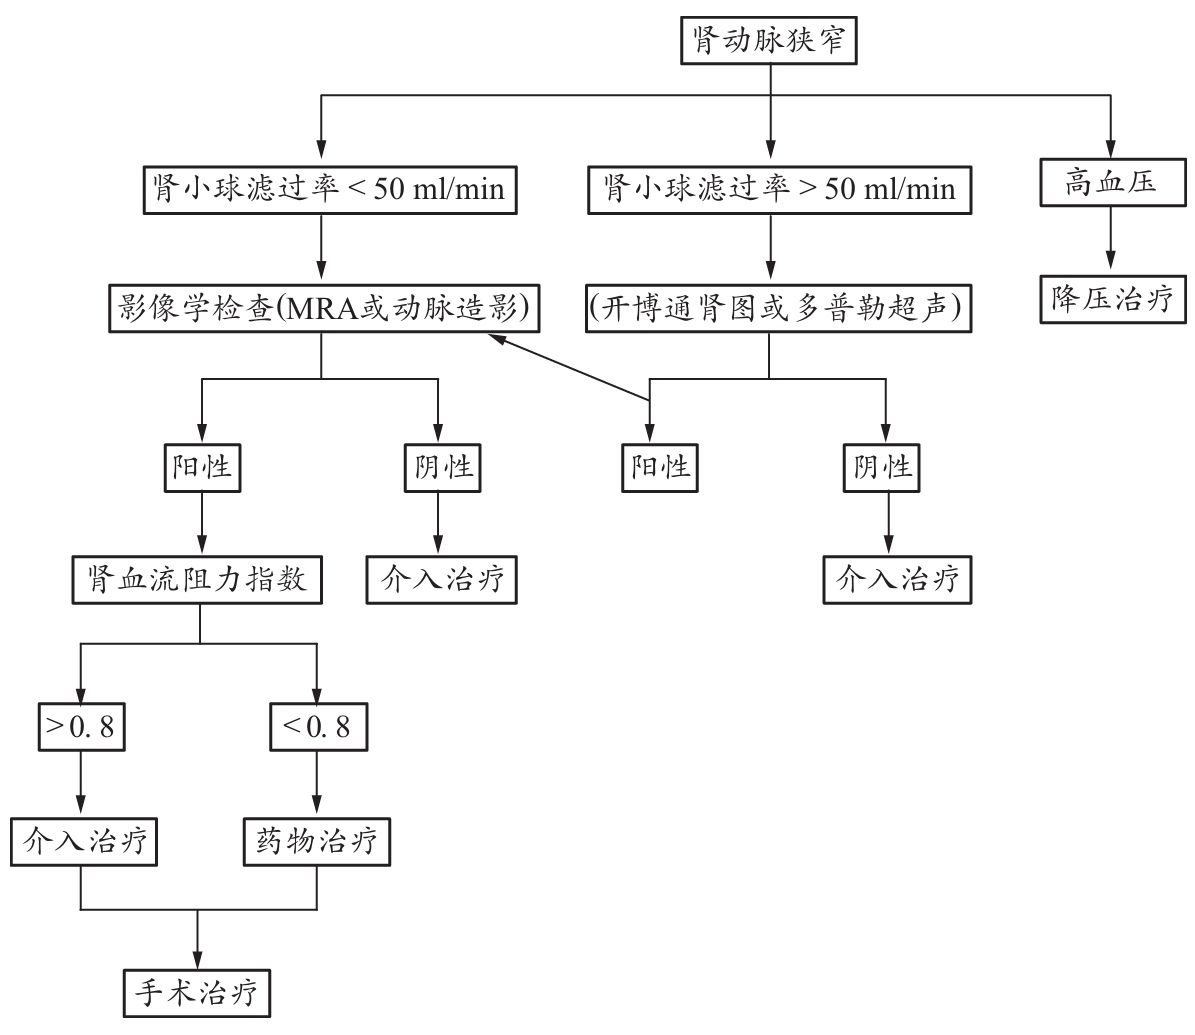
\includegraphics{./images/Image00129.jpg}
 \captionsetup{justification=centering}
 \caption{肾动脉狭窄的治疗程序}
 \label{fig4-6-1}
  \end{figure} 

【治疗方案】

1.
药物治疗 控制血压、控制血脂、降低血粘度为首选。单侧肾动脉狭窄不使用噻嗪类利尿剂,双侧肾动脉狭窄可使用速尿。谨慎使用扩张血管药物。β受体拮抗剂对于大部分高血压患者有益。降压药物的选择参见原发性高血压的治疗。阿司匹林100mg,每晚1次;氯吡格雷75mg每日1次。

2.
肾动脉扩张术(成形和内支架术) 适用于无外科手术指征的动脉粥样硬化患者。肾动脉支架置入术的适应证:①球囊血管成形术后,管腔狭窄\textgreater{}30\%。②肾动脉成形术无法解除有血流动力学意义的压力梯度。③存在肾动脉血流受限的夹层。④肾动脉开口处狭窄。⑤血管成形术后再狭窄。

3.
外科手术 包括肾脏切除和血管重建。血管重建术包括肾动脉血栓内膜切除术、主动脉肾动脉旁路术、人造血管置入术、脾肾动脉吻合术、肾动脉狭窄段切除术、病变切除及移植物置换术、肾动脉再植术和自体肾移植术。

【疗效观察与随访】

1.
观察指标 常见状态与体征、肾小球滤过率、肾血流阻力指数及影像学检查等。

2.
疗效评估 介入治疗、外科手术有望能有一定效果。显效:症状、体征消失,相关检查恢复或接近正常,半年内无复发。

3. 随访 密切观察病情变化,及时请外科会诊。

【治疗经验与解析】

1. ACEI和ARB应用需谨慎,使用时必须监测血清肌酐和血钾。

2.
服药期间需要监测GFR及血钾,4周内GFR下降\textgreater{}30\%,应停药寻找原因;如4个月内GFR下降\textless{}30\%,可继续使用。血钾≤5.5mmol/L,可继续使用。

3.
肾动脉狭窄:①一侧肾动脉狭窄,肾灌注压下降,血浆肾素水平升高,血管紧张素增加,全身血管收缩引起高血压,高血压作用于非狭窄肾,通过压力利尿作用,使钠排出增加。然而,由于血管紧张素Ⅱ增加,血管紧张素Ⅱ的血管收缩作用减少对侧非狭窄肾血流,减少GFR,对肾上腺皮质作用,促进了醛固酮生成,促进水钠重吸收,这些作用抵消了对侧非狭窄的肾脏压力利尿作用,水钠平衡只能靠全身血压升高产生的利尿作用维持。用血管紧张素转换酶抑制剂或ARB治疗后,虽然狭窄一侧肾脏血流减少,GFR下降,但对侧血流量增加,GFR增加。也就是说:对单侧肾动脉狭窄所致的肾素依赖型高血压,在用其他药物无效时,用ACEI或ARB能有效控制血压,防止并发症,但此类药物减少狭窄侧肾脏血流量,服用时应该监测肾功能变化。②双侧肾动脉狭窄高血压的主要机制是水钠潴留,特征性表现为容量扩张,血管肾素分泌被抑制,血管肾素水平正常,但是肾内肾素活性、局部血管紧张素Ⅱ增多。用ACEI或ARB后,肾内血管紧张素Ⅱ被阻断,肾小球出球动脉扩张,肾小球内压下降,使肾功能恶化。也就是说:对双侧肾动脉狭窄或孤立肾动脉狭窄所致的容量依赖型高血压,ACEI和ARB是绝对禁忌,并且疗效欠佳。

\subsection{肾动脉血栓形成}

肾动脉血栓是指肾动脉主干及其分支的血栓形成或栓塞,致肾动脉管腔狭窄或闭塞,引起肾功能恶化。肾动脉血栓可因血管壁病变(创伤,动脉粥样硬化,血管炎等)或血液高凝状态而产生。肾动脉栓塞的栓子主要来源于心脏,偶有心脏外的来源。肾动脉血栓与栓塞的病因多种多样,临床表现也各不相同,甚至无症状及体征,造成临床诊断困难。可疑病例应监测肾功能、血清酶,必要时行肾动脉造影明确诊断。早诊断,及时处理,肾功能可以完全恢复。

【治疗方案】

1.
肾动脉血栓栓塞确诊须行肾动脉造影 治疗方式有肾动脉插管局部灌注纤溶酶原激活剂溶栓、全身抗凝、外科手术取栓等方式,但局部插管溶栓治疗对发病在3日内者效果最佳,超过7日则效果较差,且容易出现溶栓相关并发症,并遗留肾功能不全。

2. 溶栓治疗

(1)静脉溶栓:效果不如动脉内溶栓确切,但因其费用少,不需介入治疗用的昂贵设备和操作技术,一般医院均可进行,因此值得推广。所有肾动脉血栓形成或血栓栓塞患者均适用。禁忌证:①高龄患者,一般认为年龄\textgreater{}75岁不宜行静脉溶栓治疗。②出血倾向。③半年内深部组织外伤或穿刺病史。④半年内脑血管意外病史。⑤溶栓剂过敏。⑥不能控制的高血压。给药方法:尿激酶或链激酶20万\textasciitilde{}40万U溶于100\textasciitilde{}500ml液体中,3小时内静脉滴注完毕。应用链激酶或尿激酶局部动脉内注入比静脉注射溶栓在肾组织仍存活的低危患者中常更有效,每日1次,连用3\textasciitilde{}7日(也有专家认为每日用量可达50万\textasciitilde{}100万U仍较安全)。溶栓过程每日监测出、凝血时间及纤维蛋白原定量。目前多数学者认为,维持纤维蛋白原在1.2\textasciitilde{}1.5g/L,凝血酶时间为正常的1.5\textasciitilde{}2.5倍,纤维蛋白降解产物在300\textasciitilde{}400mg/L最为适宜。

(2)抗凝治疗:对于有血栓形成或栓塞病史的患者,外科手术后,介入治疗和静脉溶栓治疗后的患者也应常规抗凝治疗,以防栓塞再次发生。住院患者可以给予普通肝素或相对低分子肝素静脉滴注或皮下给药。应用普通肝素时应监测:活化的部分凝血活酶时间较正常对照延长1.5\textasciitilde{}2.5倍,抗凝血酶活性维持在120\%以上以及血小板计数,严防血小板减低。低分子肝素每日一剂皮下给药可以不做监测,如静脉持续滴注,则需监测抗Xa活性。长期应用可给予华法林、噻氯匹定(力抗栓)或阿司匹林等口服抗凝药,用药剂量要求个性化,用药过程定期监测出、凝血时间,随时调整剂量,以防出血并发症。口服华法林监测的指标包括血浆凝血酶原时间维持在正常对照的1\textasciitilde{}2倍,国人INR以1.8\textasciitilde{}2.5为宜。

3. 经皮肾动脉介入术治疗 球囊扩张和支架植入术。

【疗效观察与随访】

1. 观察指标 常规症状与体征、血压、体温、血常规、AST、AKP、肾功能等。

2.
疗效评估 影响预后因素包括栓塞时间的长短、年龄和基础病。及时开展血管成形术可以避免肾梗死的发生,但成功与否多取决于缺血的时间。大多成功病例其肾缺血时间小于12小时。年轻患者创伤后肾动脉血栓若数小时不及时手术取栓,肾功能很难恢复,甚至引起死亡,而老年人在动脉粥样硬化的基础上发生肾动脉血栓,预后相对较好,肾功能多有自发恢复,其原因是在血栓发生前,肾动脉硬化及狭窄已形成许多侧支循环,减轻了血栓发生后的肾缺血。

3. 随访 密切观察病情变化,及时复查相关指标,加强医患沟通。

【治疗经验与解析】

1.
以下几点有助于早期诊断:①有发生肾动脉血栓或栓塞的可能性,包括外伤、主动脉和或肾血管造影、肾病综合征和心脏病患者。②可疑的症状及体征,如突然的腰痛、腹痛、恶心、呕吐、发热、血压升高。③化验异常,如白细胞升高,蛋白尿,镜下血尿,白细胞尿,尿酶升高,血清酶升高。④肾功能改变,出现急性少尿、无尿、急性肾衰竭。以上均应怀疑有动脉血栓栓塞并发症。确诊有赖于肾脏影像学检查。

2.
及时分析病情,及时制订治疗方案,及时采取相应的治疗措施,必要时应组织多科室会诊。

\subsection{肾静脉血栓形成}

肾静脉血栓(RVT)形成是指肾静脉主干和(或)分支内血栓形成,导致肾静脉全部或部分阻塞而引起的一系列病理生理改变和相应的临床表现。虽然外伤和肿瘤可以导致RVT,但肾病综合征是RVT形成的主要原因。肾静脉血栓可发生于单侧或双侧,主干或分支肾静脉,临床表现取决于血栓形成快慢、阻塞静脉大小、血流阻断程度及侧支循环建立与否。通常有两种表现形式:急性RVT和慢性RVT。急性RVT可出现腹痛、少尿、肉眼血尿和肾功能恶化。除肾病综合征之外,腹部肿瘤、外伤、口服避孕药、脱水(尤其是儿童)、激素治疗、肾移植术后均可诱发急性RVT形成。因纤维肌营养不良或动脉粥样硬化而存在肾动脉狭窄的患者在给予ACEI后可以诱发急性RVT形成。抗磷脂抗体综合征、凝血因子缺陷等导致机体高凝状态的诱因均可诱发急性RVT形成。慢性RVT较常见,通常临床症状不明显,仅为蛋白尿持续不缓解或增加,常伴血尿,可有肾功能受损如血肌酐升高、肾小管功能障碍,如侧支循环建立良好,肾静脉回流改善,对肾功能可无明显影响。长期随访少数可出现血栓栓塞并发症如肺栓塞。有些病例则以血栓栓塞并发症为首发表现。

【治疗方案】

1.
药物治疗 大剂量的肝素维持凝血时间是正常水平的2\textasciitilde{}2.5倍。肝素治疗5\textasciitilde{}7日后可以改为华法林口服治疗,维持凝血酶原时间是正常范围的1.5\textasciitilde{}2倍。早期急性RVT患者可考虑应用大剂量的尿激酶和链激酶局部注射。药物治疗包括:

(1)溶栓治疗:尿激酶负荷量为4400IU/kg,静注10分钟,维持量为2200IU/(kg·h),持续静脉滴注12小时;或链激酶负荷量为250000IU/kg,静脉注射30分钟,维持量为100000IU/(kg·h),持续静脉滴注24小时。

(2)抗凝治疗:可选用普通肝素,负荷量为2000\textasciitilde{}5000IU静脉注射,维持量18IU/(kg·h),持续静脉滴注然后根据APTT调整用量;或者选用低分子肝素如依诺肝素100IU/kg(那屈肝素86IU/kg或亭扎肝素175IU/kg),皮下注射,每12小时1次,持续10日。

2.
介入治疗 包括局部溶栓、取栓、滤器置入及肾动脉栓塞等。介入溶栓可以通过肾静脉和肾动脉两种途径给药,部分患者在溶栓的同时还可以配合应用取栓治疗,以便能快速去除血栓,挽救患肾。对于引起严重高血压的慢性RVT患者,可通过肾动脉栓塞达到肾截除的目的。溶栓的同时可以放置临时或永久性滤器,以防止栓子脱落造成致死率很高的肺栓塞。滤器一般放置在肾静脉开口上方的下腔静脉内。滤器置放后对肾功能一般不会造成不可逆的损伤。当然,与永久性滤器相比,临时性滤器的应用更为安全。

3.
外科手术 目前已很少被临床采用,预后改善并不明显。主要用于下列患者:①肾静脉主干内急性RVT形成,经保守治疗无效者。②双肾静脉血栓。③反复发生肺动脉栓塞。④出现严重高血压、患肾感染或患肾功能衰竭的慢性RVT患者。

【疗效观察与随访】

1.
观察指标 常见症状与体征、尿常规、肾功能、X线胸部摄片、血小板及出凝血指标等。

2.
疗效评估 本病预后取决于诊治是否及时,措施是否得力,如能及时明确诊断,及时手术可望获得显效。

【治疗经验与解析】

1.
使用尿激酶、链激酶溶栓期间勿同用肝素,溶栓治疗结束后,应2\textasciitilde{}4小时测定1次凝血酶原时间或活化部分凝血酶时间,当其水平低于正常值的2倍,即应开始规范的肝素治疗。

2.
应用肝素/低分子肝素前应了解有无禁忌证。使用肝素时应监测APTT,具体监测方法可参见肺血栓栓塞章节,使用低分子肝素无需监测APTT,但疗程\textgreater{}7日需监测血小板。

\section{急性肾功能衰竭}

急性肾衰竭(ARF)是由各种原因引起的肾功能在短时间内(几小时至几周)突然下降而出现的氮质废物滞留和尿量减少综合征。肾功能下降可发生在原来无肾脏病的患者,也可发生在慢性肾脏病(CKD)患者。ARF主要表现为氮质废物血肌酐(Cr)和尿素氮(BUN)升高,水、电解质和酸碱平衡紊乱,及全身各系统并发症。常伴有少尿(\textless{}400ml/d),但也可以无少尿表现。最近对这一综合征有了新的认识,定义为急性肾损伤(AKI):48小时内血肌酐上升≥0.3mg/dl或较原先水平增高50\%和(或)尿量\textless{}0.5ml/(kg·h)时间\textgreater{}6小时(排除梗阻性肾病或脱水状态),并进行分期(表\ref{tab4-7-1})。

\begin{table}[htbp]
    \centering
    \caption{AKI的分期标准---------2005年急性肾损伤协作组(AKIN)}
    \label{tab4-7-1}
    \begin{tabular}{lp{6.3cm}p{5cm}}
\toprule
分期 & 血清肌酐标准 & 尿量标准\tabularnewline
\midrule
\rowcolor{lightgray}1期 & 绝对升高≥0.3mg/(d·L)或相对升高≥50\% &
\textless{}0.5ml/(kg·h)(时间\textgreater{}6h)\tabularnewline
2期 & 相对升高\textgreater{}200\%\textasciitilde{}300\% &
\textless{}0.5ml/(kg·h)(时间\textgreater{}12h)\tabularnewline
\rowcolor{lightgray}3期 &
相对升高\textgreater{}300\%或在≥4.0mg/(d·L)基础上再急性升高≥0.5mg/(d·L)
& 少尿[\textless{}0.3ml/(kg·h)]×24h或无尿×12h\tabularnewline
\bottomrule
    \end{tabular}
\end{table}

【治疗程序】 如图\ref{fig4-7-1}所示。

\begin{figure}[!htbp]
 \centering
 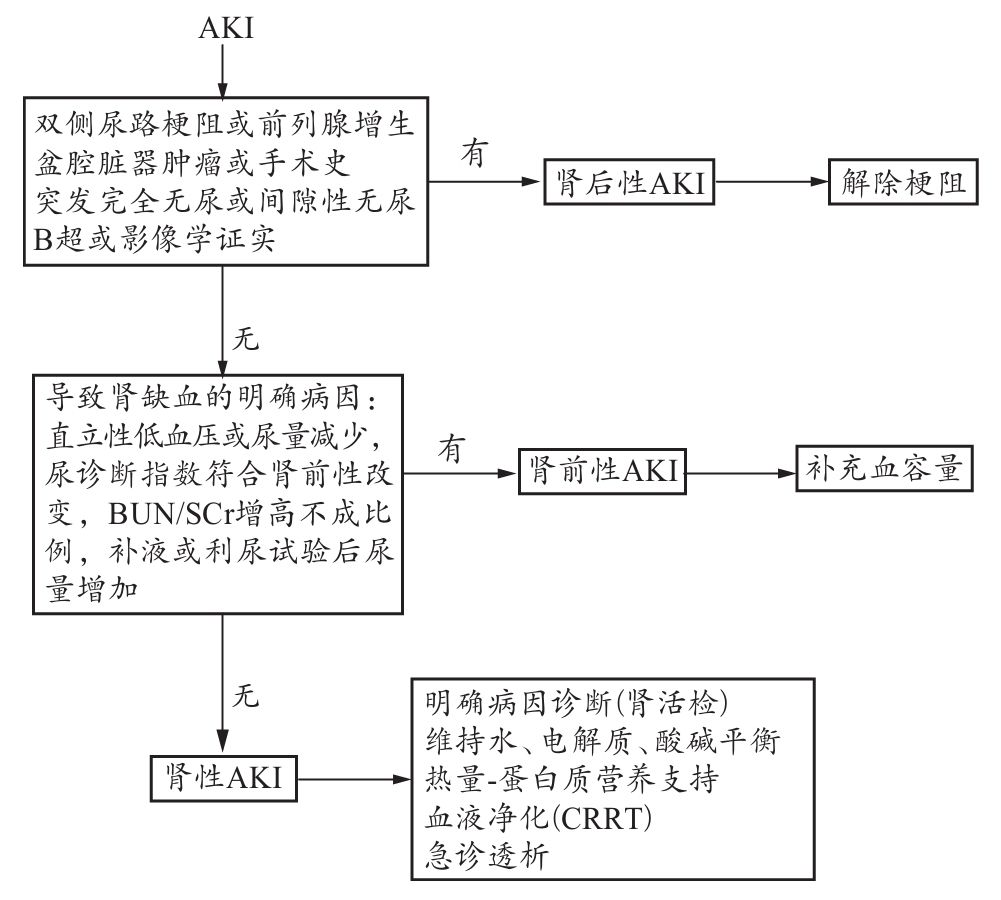
\includegraphics{./images/Image00130.jpg}
 \captionsetup{justification=centering}
 \caption{急性肾功能衰竭的治疗程序}
 \label{fig4-7-1}
  \end{figure} 

【治疗方案】

1.
对于AKI的一、二级预防是最重要的 必须对发病的高危人群,包括老年人、原有肾脏疾病患者、采取特殊检查或治疗措施者(血管造影、肿瘤化疗、造血干细胞移植、器官移植、特殊抗生素使用等)给予相应保护措施并密切跟踪病程中尿量、血肌酐的动态变化,以期早诊断、早治疗。

2.
纠正可逆的病因 早期干预治疗ARF首先要纠正可逆的病因。对于各种严重外伤、心力衰竭、急性失血等都应进行相关治疗,包括输血,等渗盐水扩容,处理血容量不足、休克和感染等。停用影响肾灌注或肾毒性的药物。

3.
维持体液平衡 每日补液量应为显性失液量加上非显性失液量减去内生水量。由于非显性失液量和内生水量估计常有困难,因此每日大致的进液量,可按前一日尿量加500ml计算。发热患者只要体重不增加可增加进液量。

4.
饮食和营养 ARF患者每日所需能量应为每公斤体重147kJ(35kcal),主要由碳水化合物和脂肪供应;蛋白质的摄入量应限制为0.8g/(kg·d),对于有高分解代谢或营养不良以及接受透析的患者蛋白质摄入量可放宽。尽可能地减少钠、钾、氯的摄入量。不能口服的患者需静脉营养补充必需氨基酸及葡萄糖。

5.
高钾血症 血钾超过6.5mmol/L,心电图表现为QRS波增宽等明显的变化时,应予以紧急处理,包括:①钙剂(10\%葡萄糖酸钙10\textasciitilde{}20ml),稀释后静脉缓慢(5分钟)注射。②11.2\%乳酸钠或5\%碳酸氢钠100\textasciitilde{}200ml,静滴。③50\%葡萄糖溶液50\textasciitilde{}100ml,加普通胰岛素6\textasciitilde{}12U缓慢静脉注射。④口服离子交换(降钾)树脂15\textasciitilde{}30g,每日3次。⑤以上措施无效或为高分解代谢型ATN的高钾血症患者,透析是最有效的治疗方法。

6. 代谢性酸中毒 应及时治疗,如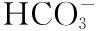
\includegraphics{./images/Image00128.jpg}
低于15mmol/L,可选用5\%碳酸氢钠100\textasciitilde{}250ml静滴。对于严重酸中毒患者,应立即开始透析。

7.
感染 应尽早使用抗生素。根据细菌培养和药物敏感试验选用对肾无毒性或毒性低的药物,并按肌酐清除率调整用药剂量。

8.
透析疗法 可选择腹膜透析(PD)、间歇性血液透析(IHD)或连续性肾脏替代治疗(CRRT)。腹膜透析无需抗凝和很少发生心血管并发症,适合于血流动力学不稳定的患者,但其透析效率较低,且有发生腹膜炎的危险,在重症ARF已少采用。血液透析的优点是代谢废物的清除率高、治疗时间短,但易有心血管功能不稳定和症状性低血压,且需要应用抗凝药,对有出血倾向的患者增加治疗的风险。CRRT包括连续性动静脉血液滤过(CAVH)和连续性静静脉血液滤过(CVVH)等一系列方法,适用于多器官功能衰竭患者,具有血流动力学稳定,每日可清除水10\textasciitilde{}14L或更多,保证了静脉内高营养。但要注意监护,注意肝素用量。

9.
多尿的治疗 多尿开始时,由于肾小球滤过率尚未恢复,肾小管的浓缩功能仍较差,治疗仍应维持水、电解质和酸碱平衡,控制氮质血症和防止各种并发症。已施行透析的患者,仍应继续透析。多尿期1周左右后可见血肌酐和尿素氮水平逐渐降至正常范围,饮食中蛋白质摄入量可逐渐增加,并逐渐减少透析频率直至停止透析。

【疗效观察与随访】

1. 观察指标 常见症状与体征、尿常规、肾功能、电解质等。

2.
疗效评估 治愈标准:症状、体征消失,肾功能恢复至正常范围,半年内无复发。

3. 随访 对好转者定期复查尿常规、肾功能,指导保健措施。

【治疗经验与解析】 AKI早期、正确、全面的诊断非常重要,直接影响治疗效果和预后。急性肾损伤诊断看似简单,只有1\textasciitilde{}2个指标,但真正做到早期正确全面的诊断较为困难,原因包括:①血肌酐本身不够敏感。②很多患者AKI病因是多因素的。③同一患者在病史的不同阶段病因会有转换。④AKI可以出现多种并发症,并发症是AKI的加重因素或新的病因。

因此,除要根据肌酐进行分层诊断外,还要做如下分层诊断:①确定是否存在AKI(保证肾灌注的情况下)。②确定是单纯AKI或是慢性肾损伤基础上的急性加重。③详细了解肾前性相关因素和除外经典肾后性疾病。④分析肾实质性AKI。⑤注意特殊疾病的诊断。⑥AKI并发症预防和诊断。

以上各层诊断的基础均为详尽的病史,较为重要。其次是各种血、尿和影像学等相应检查,虽然病患最终可能通过肾活检得到明确诊断,但上述各病理生理过程和特点仍需重视。

只有及时正确全面的诊断,才能保证改善AKI预后和降低急性肾损伤病死率。

\section{慢性肾功能衰竭}

各种慢性肾实质疾病逐渐进展,就会缓慢出现肾功能减退最终至慢性肾衰竭(慢肾衰)。慢肾衰是一个临床综合征,国内根据肾功能损害的程度可分为肾功能不全代偿期、肾功能不全失代偿期、肾功能衰竭期、尿毒症期;现在多沿用美国K/日OQI慢性肾脏病临床实践指南将慢性肾脏病(CKD)分为5期,其分类依据的是肾小球滤过率[GFR,单位ml/(min·1.73m{2}
)]水平:1期:GFR≥90;2期:GFR 60\textasciitilde{}89;3期:GFR
30\textasciitilde{}59;4期:GFR
15\textasciitilde{}29;5期:GFR\textless{}15(或透析)。

【治疗程序】 如图\ref{fig4-8-1}所示。

\begin{figure}[!htbp]
 \centering
 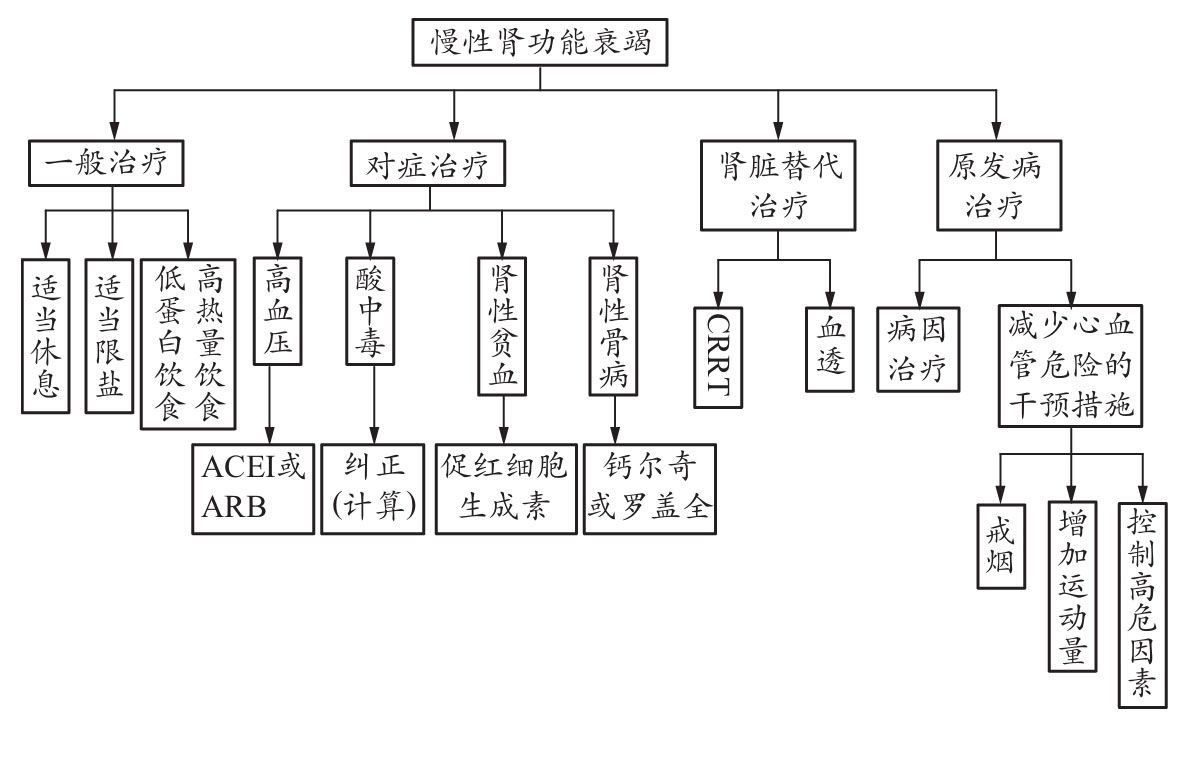
\includegraphics{./images/Image00131.jpg}
 \captionsetup{justification=centering}
 \caption{慢性肾功能衰竭的治疗程序}
 \label{fig4-8-1}
  \end{figure} 

【治疗方案】

1.
肾功能不全的降压原则及药物选择 ①生活方式改变,包括盐的摄入。②药物选择:降压首先以肾素-血管紧张素-醛固酮拮抗剂为中心。③往往需要多种降压药物联合治疗。

对于糖尿病肾病无论ACEI或ARB均存在大量循证医学证据肯定其降低蛋白尿和肾脏保护作用,对于非糖尿病肾病型RCT研究主要是针对伴有大量蛋白尿和肾功能受损的患者,ACEI对于肾功能保护作用是否优于其他降压药物仍然存在争议。2008年一项荟萃分析表明在6\textasciitilde{}12个月降低蛋白尿方面ACEI与ARB疗效相似。K/DOQI推荐加用中大剂量ACEI或ARB,以更好的降低蛋白尿和保护肾功能,通常应用常规剂量2倍以上,即使不能进一步降低系统血压,亦有助于进一步降低蛋白尿。关于ACEI和ARB联合治疗是否优于单药治疗,目前仍然存在争议。低盐摄入或者加用少量利尿剂可增强RAAS拮抗剂降低血压和蛋白尿的疗效,通常要求24小时尿钠不超过100mmol。钙通道阻滞剂降压作用强,不受食盐摄入量影响,在ACEI和利尿剂应用血压仍不达标可加用非二氢吡啶类。CKD患者肾功能受损时,交感神经活性增强,加用α受体拮抗剂和β受体拮抗剂除协助控制血压,还可能起到抑制交感神经的作用,可能对患者长期预后有益。

2.
慢性肾功能不全患者减少心血管危险性的干预措施 干预传统危险因素包括戒烟、适当增加运动、控制糖尿病、控制高血压和限制饮食,给予他汀类药物使LDL-胆固醇\textless{}100mg/dl。干预非传统危险因素包括减轻细胞外液容量负荷过度,确定合适的干体重;用促红素和铁剂治疗贫血,使血红蛋白在110\textasciitilde{}120g/L之间;防治炎症和低蛋白血症;用他汀类药物治疗脂质代谢紊乱;治疗二价离子代谢紊乱,使血清钙维持在9.2\textasciitilde{}9.6mg/dl;血清磷维持在2.5\textasciitilde{}5.5mg/dl,iPTH
100\textasciitilde{}200pg/ml;伴有冠状动脉疾病、血管疾病或糖尿病给予抗血小板制剂;合理应用ACEI或ARB治疗蛋白尿和小动脉硬化;已有缺血性血管疾病者给予ACEI和β受体阻滞剂。

3.
慢性肾功能不全肾性贫血的治疗 建议所有透析患者以及透析前的CKD患者,当Hb≤10g/dl时开始促红细胞生成素治疗,起始剂量为每周80\textasciitilde{}120IU/kg,常用剂量为6000\textasciitilde{}9000IU,分2\textasciitilde{}3次皮下注射,静脉应用时需要增加剂量30\%\textasciitilde{}50\%,以弥补静脉使用的半衰期比皮下注射缩短所致的疗效减弱。ESA治疗的副作用为高血压、透析通路血栓、高钾血症、纯红再障。促红素低反应的常见原因为剂量不足、感染、慢性失血、继发性甲状旁腺功能亢进、骨髓纤维化、肿瘤、铝中毒、营养不良、透析不充分、血红蛋白病、溶血、叶酸或维生素B{12}
缺乏以及使用ACEI/ARB。

4. 慢性肾功能不全矿物质代谢紊乱和骨病的治疗

(1)控制高磷血症:每日磷摄入量应当小于800\textasciitilde{}1000mg,如血磷仍不能达标可使用磷结合剂碳酸钙、醋酸钙、司维拉姆在进餐同时口服,对于有高钙血症或者连续2次血iPTH水平低于150pg/ml或者存在严重软组织尤其血管钙化和(或)动力缺失性骨病的患者应当选用不含钙的磷结合剂。血磷高于7.0mg/dl时可以短期应用含铝的磷结合剂,但是不要超过4周。

(2)纠正低钙血症,防止高钙血症:患者每日的总钙摄入量不要超过2000mg。

(3)补充维生素D或类似物治疗SHPT:当校正血钙超过10.2mg/dl或者持续存在高磷血症时应当停止一切维生素D的治疗,直到血钙下降到9.5mg/dl以下,血磷下降到4.6mg/dl以下才可以再次开始。

(4)应用治疗骨质疏松药物如二膦酸盐或生长激素治疗骨病。

(5)纠正酸中毒。

(6)甲状旁腺切除术:对于伴有高钙和(或)高磷血症,药物治疗无效的严重SHPT患者,iPTH水平持续高于800pg/ml应考虑行甲状旁腺次全切除术,或者甲状旁腺全切术加自体移植。

(7)及早发现血管钙化。

5. 慢性肾功能不全的营养治疗

(1)增加营养物质的补充,口服优于鼻饲和全胃肠外营养;GFR25\textasciitilde{}60ml/min时,DPI0.6\textasciitilde{}0.75g/(kg·d);GFR\textless{}25ml/min时,DPI0.6g/(kg·d)。

(2)避免导致炎症反应的诸多因素。

(3)促进合成代谢。

6. 其他治疗

(1)用ACEI时需监测肾功及血钾变化,并避免与利尿剂合用,当血Cr达266μmol/L以上时应停用,肾动脉狭窄者勿用。服用ARB也应监测血钾水平。

(2)开同含钙元素,如同时口服补充其他钙剂及活性维生素D时,要定时测血钙浓度。

(3)服用骨化三醇或阿法D{3} 时,应每2周测钙1次,防止高钙血症。

(4)由于氢氧化铝在慢性肾衰竭患者体内易蓄积致铝中毒,故现已多不用其作为磷结合剂。

(5)EPO以皮下注射效果好。当血HCT达到30\%\textasciitilde{}35\%,Hb达100g/L时,应减少剂量。用EPO时注意充分纠正铁缺乏,否则影响疗效。继发甲旁亢、慢性感染、营养不良、铝中毒、叶酸及维生素B{12}
缺乏亦影响EPO疗效。有人认为ACEI也影响EPO疗效。

(6)慢性肾衰竭合并急性左心衰肺水肿时,用洋地黄类制剂效果差,同时如果患者已无尿用呋塞米无效。大剂量用呋塞米时应慢推,否则可能有暂时性耳聋。抢救肺水肿最有效方法是超滤脱水。

(7)处理慢性肾衰竭高钾血症时,应先推钙,后补碱,否则可引起低钙抽搐,当血钾大于6.5mmol/L时,血透是最有效的方法。

(8)口服胃肠透析仅是不得已方法,清除尿毒症毒素效果远不如透析。在有活动性消化道出血时禁用。

(9)继发性甲旁亢有时可与铝中毒并存,应先处理铝中毒。DFO治疗的副作用有过敏反应和低血压。

【疗效观察与随访】

1.
观察指标 常见症状和体征、血压、肾功能、尿常规、血钙、血磷、血象、电解质、血气、CO{2}
P等。

2.
疗效评估 好转标准:症状、体征改善,肾功能改善,并发症缓解或完全控制。

3.
随访 密切观察病情变化,定期复查相关指标,一旦病情恶化,立即去医院诊治。

【治疗经验与解析】

1.
KD早期的防治重点应落实在高危人群及疾患者群的长期追踪、医疗管理和指导。对每一个CKD患者的随诊应包括:

(1)3个月后复查尿微量白蛋白,确认是否可诊为CKD及其分期;进行病因学检查,判断原发的肾脏疾病及其干预治疗的可能措施;

(2)CKD患者应至少每年检测1次血肌酐以评估GFR。GFR下降的程度有很大的个体差异性,如大部分研究提示男性患者、老年患者进展较快;更与原发病的类型有关,如多囊肾进展快,肾小球疾病比肾小管间质肾病进展速度更快。目前CKD的防治还主要在其二级预防阶段。循证医学证实,在CKD的1、2期通过治疗高血压、应用血管紧张素Ⅱ转化酶拮抗剂降低尿蛋白;在CKD3期通过纠正贫血、钙磷代谢紊乱等措施,可以延缓肾脏功能的损害,减少心血管合并症和CKD患者总体死亡率;对于纠正高血脂的作用尚有争议。根据每个患者原发病、CKD的分期、合并症的情况制定具体防治措施,每1\textasciitilde{}6个月监测措施的效果及不良反应以调整方案。

2.
CKD高血压治疗以控制血压达标为宗旨,在CKD4、5期的患者,常需用2\textasciitilde{}3种降压药,应用RAAS阻断剂时应注意:①ACEI/ARB加量过程中注意监测血肌酐较基线升高超过30\%(一般发生在开始用药2\textasciitilde{}4周内,或用药过程中出现呕吐、腹泻等脱水状态;加用NSAID、利尿剂时),则应减量或停用。寻找可能的原因调整状态后可再次用药。②对于晚期CKD患者应用ACEI和(或)ARB应警惕高钾血症,应密切随访、低钾饮食、避免合用NSAID药物,必要时给予相应急救。

3.
对于所有透析患者以及透析前患者,当Hb≤10g/dl时开始促红细胞生成素治疗。起始剂量为每周80\textasciitilde{}120IU/kg,治疗应使Hb每月上升约1g/dl,3\textasciitilde{}4个月达标。如果4周内Hb增加\textgreater{}2.5g/dl,应该减少剂量20\%\textasciitilde{}50\%。如果在铁储备充足的情况下4周内Hb增加\textless{}1g/dl,则增加剂量25\%。促红细胞生成素低反应的常见原因为剂量不足,感染和(或)炎症,慢性失血,继发性甲状旁腺功能亢进,骨髓纤维化,肿瘤,铝中毒,营养不良,透析不充分,血红蛋白病,溶血,叶酸或维生素B{12}
缺乏,使用ACEI和(或)ARB。使用促红素治疗前及治疗中应补充铁剂,血液透析患者应每月监测铁指标,腹膜透析及透析前的患者每2个月监测1次。2006年DOQJ要求血清铁维持在200\textasciitilde{}600μg/L最佳范围内,转铁蛋白饱和度\textgreater{}20\%。在促红素治疗的初始3个月内大约需要补充1000mg铁,以后每月需要25\textasciitilde{}100mg铁。

4.
减少蛋白尿是CKD治疗的目标。根据大型RCT研究结果,ACEI和ARB是治疗蛋白尿最重要的药物。对进展性CKD患者采用多种危险因素干预以降低蛋白尿是合理的。

5.
对于CKD3\textasciitilde{}5期患者,可以定期进行超声心动图检查并关注是否存在瓣膜钙化,也可以进行CT检查来评价血管钙化,此外侧位腹部X线片可以作为替代CT的选择。

6.
CKD4\textasciitilde{}5期后常出现蛋白质能量营养不良,其发生率在血透为10\%\textasciitilde{}70\%,发生率在腹透为18\%\textasciitilde{}50\%。蛋白质能量消耗表现在血清白蛋白、前白蛋白、胆固醇的下降,身体重量下降,肌肉重量下降。治疗措施为增加营养物质的补充、抗炎、促进合成代谢。

\section{梗阻性肾病}

梗阻性肾病是由泌尿道结构和(或)功能异常,引起尿液或肾小管液排出受阻,导致肾内压力增高,引起肾小管间质病变和肾功能损害的一组临床综合征。是儿童和老年慢性肾功能衰竭的常见原因。10岁以下儿童,男性多见,多由先天性畸形引起,10\textasciitilde{}20岁患者发病率男女比例大致相同,20岁以上患者,女性多见,多为妊娠和妇科恶性肿瘤引起,60岁以上男性主要为良性前列腺增生和前列腺癌。根据梗阻发生部位、程度、持续时间的不同,临床表现差异很大,上尿路梗阻可表现为疼痛或梗阻后肾小球和小管功能变化,下尿路梗阻表现为排尿困难、尿量改变或肾功能衰竭。患者还可出现腹部包块和反复尿路感染。

【治疗程序】 如图\ref{fig4-9-1}所示。

\begin{figure}[!htbp]
 \centering
 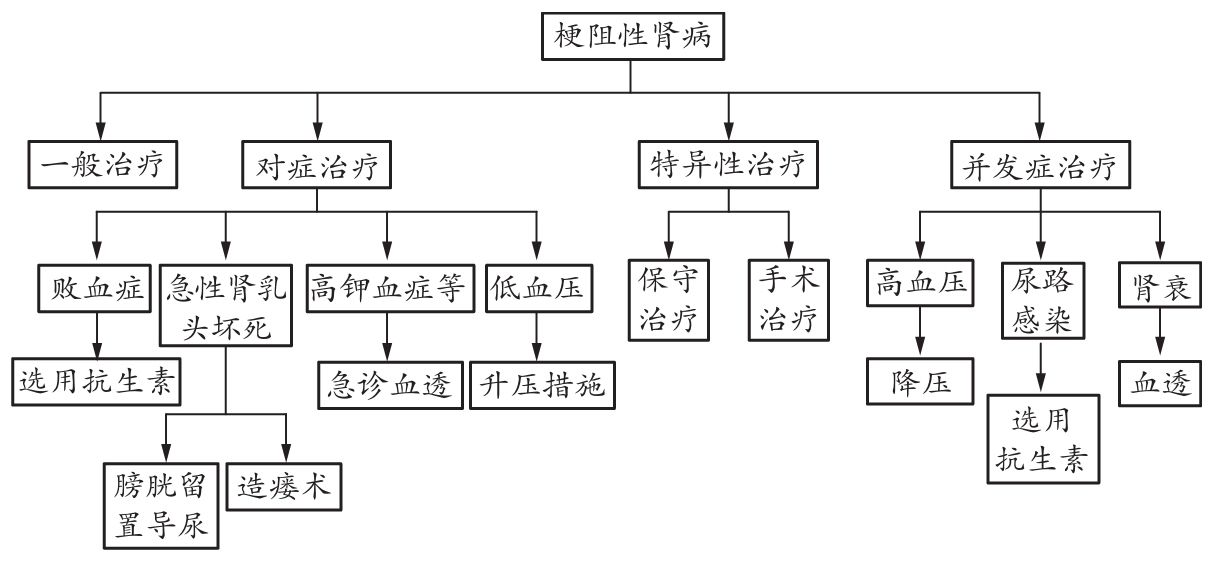
\includegraphics{./images/Image00132.jpg}
 \captionsetup{justification=centering}
 \caption{梗阻性肾病的治疗程序}
 \label{fig4-9-1}
  \end{figure} 

【治疗方案】 治疗原则为尽早明确诊断,结石解除梗阻,防治尿路感染等并发症,挽救和恢复肾功能,并对病因进行治疗。这往往需要肾内科医生与泌尿外科专家的密切协作。

1. 积极处理危及生命的各种急重症

(1)G{-} 菌败血症:重度不全梗阻或完全性梗阻时,肾盂肾炎可进展至G{-}
菌败血症。当患者出现发热时,立即予血、尿细菌培养,在培养结果回报前即静脉使用强有力抗生素治疗。

(2)急性肾乳头坏死:肾盂肾炎及梗阻可继发急性肾乳头坏死,导致肾组织的快速毁损,此时应急诊外科处理减轻梗阻,如膀胱留置导尿术或经皮肾穿刺造瘘术。

(3)高钾血症等合并症:梗阻性肾病致急或慢性肾衰竭,合并高钾血症、酸中毒、抽搐、昏迷、心包炎等危及生命的情况时,应急诊透析治疗,待患者病情允许后再纠正梗阻。

(4)低血压:少数情况下,梗阻后利尿及慢性不全梗阻患者液体摄入不足,可出现血管收缩,低血压,注意纠正。

2.
解除梗阻,挽救肾功能 一旦明确存在梗阻,常需尽快解除梗阻。解除梗阻的方式取决于梗阻的位置、程度、病因以及合并症或并发症。梗阻解除后应进一步针对梗阻原因进行治疗。

(1)下尿路梗阻:常见为良性前列腺增生症,或尿道狭窄,可予留置导尿解除梗阻。如果导尿管无法通过狭窄处,可予耻骨联合上膀胱造瘘术。

(2)上尿路梗阻:狭窄部位在输尿管膀胱连接处以上,可使用经皮肾盂造瘘术,膀胱镜逆行输尿管插管并行支架安置术等先行解除梗阻。不过对于恶性肿瘤外压所致上尿路梗阻,输尿管支架效果较差。

是否急诊解除梗阻,应根据肾功能衰竭程度,有无感染,手术总体风险等综合权衡。出现以下情况时,应考虑急诊干预解除梗阻:梗阻侧泌尿道感染难以局限,发热,尿路感染源性败血症,难以控制的肾绞痛,重度梗阻,急性肾衰竭伴双侧输尿管梗阻或孤立肾梗阻。

3. 明确梗阻病因,进行特异性治疗

(1)肾盂梗阻:有症状的先天性输尿管肾盂梗阻患者(腹痛或腹块),反复尿路感染者,肾功能进行减退患者,可予手术治疗。此外,应去除外压性的损伤,例如肾动脉异常等。外科治疗包括输尿管肾盂成形术,术后影像学检查发现肾盂外形无明显改善,但肾功能减退的速度以及尿路感染可明显减少。对于存在肾盂扩张及轻度肾盂输尿管梗阻、但肾功能稳定的患者,可暂不需要手术。

若肾结石阻塞肾盂输尿管连接处数天,通常需要外科手术治疗,因为结石无法自行通过,可能导致肾功能进行性损害。肾盂或肾盏内的小结石通常不需外科去除,除非出现间断性的尿路梗阻,因为这些小结石难以定位,手术相关的肾损害风险明显增高。对大的、未导致梗阻的鹿角形结石,外科治疗存在争议,因为外科手术难度很大,而且,除非所有的感染性结石碎片都已清除,并且预防感染复发,否则很容易再次形成结石。

(2)输尿管梗阻:肾结石是成人输尿管梗阻常见原因。如果直径小于5\textasciitilde{}7mm,大多数结石可自行通过,甚至更大的结石有时也能自行通过。因此,如果不存在感染,可先通过镇痛药和多饮水以控制这类结石。如果结石下移至输尿管更低的位置,可在膀胱镜下用套石网篮取石,如果结石在输尿管更高位置,则可能需输尿管切开取石。直径7\textasciitilde{}15mm结石,可采用体外冲击波碎石。90\%患者,结石碎片在3个月内排出。大多数患者体外冲击波碎石治疗后2\textasciitilde{}3日可重返工作岗位。其他原因所致的输尿管梗阻,如结核挛缩或肿瘤、腹膜纤维化的外源性压迫,通常需要进一步的手术治疗。

(3)下尿路梗阻:下尿路症状进行性加重、反复严重的尿路感染、尿潴留或肾功能进行性恶化者,需选择外科修复。但仅有膀胱残留尿、轻到中度的膀胱输尿管反流、或肾盂扩张并非必须手术治疗。理想的外科治疗应去除梗阻,并重建泌尿道的连续性。然而,在很多情况下,梗阻性损害无法切除,尿流改道需要数周甚至数年的时间。根据病情的不同,可选用间断或持续膀胱导尿、经皮肾穿刺造瘘术、肾盂造瘘术、输尿管皮肤造瘘术、耻骨联合上膀胱造瘘术、膀胱尿道吻合术以及其他一些手术,但是每种方式都有出现再次梗阻、逆行尿路感染、电解质紊乱、容量不足、肾结石等并发症的风险。如果肾功能无法恢复,可行肾切除术。

(4)需要切除肾脏的一些情况:单侧输尿管梗阻并反复难治性肾盂肾炎,但肾仍有功能时,不一定需将肾脏切除。因为肾盂肾炎可能逆行感染至对侧未梗阻肾脏,若此时切除有功能的肾组织,会加重慢性肾衰竭的进展。如果单侧输尿管梗阻并反复的、严重的、难治性肾盂肾炎,但梗阻侧肾功能已经发生严重的不可逆损害,需行肾切除术。有功能的梗阻肾仅在外科修复失败、该侧肾脏成为危及生命的G{-}
菌败血症的感染源时才考虑切除。

4. 并发症的内科治疗

(1)尿路感染:梗阻性肾病患者合并尿路感染时通常很难根治。急性的尿路感染,无论有或无肾盂肾炎的临床表现,都应该做尿菌培养,选用适当的抗生素治疗,根据药敏结果和治疗反应调整抗生素的使用。应选用在肾组织和尿液中浓度高的抗生素。梗阻性肾病患者,尿路放置导管等时可在术前1h及术后数小时内预防性静脉使用抗生素。对于慢性梗阻或鹿角形结石的患者,长期预防性使用抗生素可减少肾盂肾炎的发生。

(2)高血压和肾衰竭:单侧急性梗阻患者肾素分泌增多,双侧肾积水患者多由水、钠潴留所致,梗阻性肾病相关的高血压,治疗上通常选用降压药,如钙离子通道阻滞剂或血管紧张素转换酶抑制剂。对于梗阻所致的急性肾衰竭或终末期肾病,可选用透析治疗。梗阻所致的终末期肾病也适合肾移植治疗,但通常需要将双侧肾脏切除,以减少感染复发。

(3)水、电解质紊乱:尿路梗阻可导致肾小管功能障碍,使尿中氯化钠、碳酸氢钠等丢失过多。此外,由于肾小管功能损害,尿液中水分丢失过多,甚至出现肾性尿崩。治疗上可相应地给予氯化钠和(或)碳酸氢钠口服,以及大量饮水。如并发腹泻、呕吐或大量出汗时,尤其注意补液。完全性梗阻或严重的不全梗阻解除梗阻时,可出现梗阻后利尿,此时尤其应密切监测电解质、输液量、尿量及体重变化,维持水、电解质平衡,补充水、氯化钠、碳酸氢钠、钾等。容量恢复正常后,液体的补充应包括尿液丢失部分及不感蒸发。

【疗效观察与随访】

1.
观察指标 常见症状与体征、血压、肾功能、电解质、血象、尿常规、尿培养等。

2.
疗效评估 完全性梗阻,1周内解除,肾功能可完全恢复,完全性梗阻2周,梗阻解除后3\textasciitilde{}4个月,GFR恢复至70\%,完全性梗阻4周,梗阻解除后,GRF仅能恢复至30\%,完全性梗阻超过6周,梗阻解除后,肾功能极难恢复,完全性梗阻超过8周,肾功能几乎完全丧失。

3.
随访 对已行手术治疗梗阻或慢性梗阻患者,需要密切的长期随访,随访项目包括临床评估,尿液检查,尿液培养,定期影像学检查等,最为重要的是,定期检查肾功能,通常用内生肌酐清除率的方法评估肾功能。

【治疗经验与解析】

1.
慢性梗阻性肾病重度积水患者,IVU检查常不显影,肾脏常被认为无功能,但即使皮质厚度小于2cm,肾核素显像仍可见浓集影,提示IVU评估肾功能并不准确,可予SPECT肾动态显像检查,或64层螺旋CT灌注成像评价肾功能。

2.
产前诊断重度胎儿肾积水患者出生后1\textasciitilde{}2周应常规行B超、CTU或MRU及SPECT检查明确诊断。确诊存在器质性梗阻的新生儿,若重度肾积水,分肾功能小于35\%或并严重的泌尿系统感染者,应尽早手术干预。

3.
双J管具有内引流和内支架作用,超声是留置术后随访的可靠方法,有助于临床制定相应的处理措施并缩短换管或拔管时间,减少并发症发生。

\section{肾石症}

泌尿系统内的结石称为肾石症、尿石症或泌尿系结石。根据结石位置的不同,将肾盂或肾盏内的结石称为肾结石,输尿管内的称为输尿管结石(进一步可分为上、中、下输尿管结石),下尿路(膀胱)结石趋少见。肾石症临床表现差异较大,轻者无症状,典型者表现为疼痛和血尿、尿路感染等,严重者甚至出现肾功能损害,且肾结石具有复发的特点。诸多因素可引起泌尿系结石,在我国,上尿路结石比下尿路结石多,其中上尿路结石主要为肾结石,故本章主要讨论肾结石。

【治疗程序】 如图\ref{fig4-10-1}所示。

\begin{figure}[!htbp]
 \centering
 
\includegraphics{./images/Image00133.jpg}
 \captionsetup{justification=centering}
 \caption{肾石病的治疗程序}
 \label{fig4-10-1}
  \end{figure} 

【治疗方案】

1. 非手术治疗

(1)止痛:首先应减轻患者疼痛,控制症状。随机对照试验结果表明非甾体消炎药(NSAID)与麻醉剂同等有效,可首选双氯芬酸钠,50mg,每日3次,连续7日,在治疗前4日效果比较明显,并可有效防止疼痛再次发作,或选用布洛芬、吲哚美辛等。其次选用盐酸氢吗啡酮+阿托品,曲马多,喷他佐辛等治疗。对输尿管结石可能自行排出的患者,双氯芬酸钠50mg,每日2次,连续3\textasciitilde{}10日,可明显减轻炎症和疼痛再发风险。双氯芬酸钠可能影响肾功能已异常患者的肾功能,但对肾功能正常患者无影响。

(2)排石治疗:大量饮水有助于结石排出,饮水\textgreater{}2\textasciitilde{}3L/24h,使尿量\textgreater{}2L/24h可加速结石排出。α{1}
受体阻滞剂或钙离子通道阻滞剂可抑制输尿管痉挛,促进输尿管结石的自发性排出。α{1}
受体阻滞剂包括坦索罗辛、阿夫唑嗪、特拉唑嗪等。钙离子通道阻滞剂以尼非地平为代表。与单独水化治疗相比,尼非地平可使结石通过率提高9\%,α{1}
受体阻滞剂可提高29\%。糖皮质激素(如甲泼尼龙16mg/d)可减轻结石所致的输尿管水肿,与α{1}
受体阻滞剂或钙离子通道阻滞剂联用,可能进一步提高结石的排出率,但不提倡单剂使用激素。排石治疗对远端输尿管结石治疗效果尚可,但对于近端及肾结石等仍有待研究。对于直径小于1cm,且症状已控制的患者,可观察4周排石治疗效果,无效应考虑侵入治疗,以免出现并发症及肾功能损害。

2. 手术治疗 取决于泌尿系结石的大小、位置、症状和体征,有无梗阻等情况。

(1)体外冲击波碎石(ESWL):是目前最常用的泌尿系结石治疗方法。体外冲击波碎石可用于直径小于2cm,尤其对非肾盏下极肾结石的治疗。ESWL对肾盂结石最为有效,无石率可达76\%,但对肾盏下极的结石效果最差。因此,对下极的结石,仅直径小于1cm时使用体外冲击波碎石治疗。近端输尿管结石也可选用体外冲击波碎石。以往该部位输尿管镜较难达到,但随着输尿管镜技术改进后,现也可以到达该部位。ESWL存在一些缺点:可能损伤弹道附近结构,导致出血、炎症或穿孔。在治疗过程中也可能引起心律失常。在孕妇和出血性疾病患者禁忌使用,病理性肥胖患者效果不佳。如果结石距皮肤距离超过10cm,或下极结石与输尿管成锐角,或过度肥胖、BMI大于30kg/m{2}
,体外冲击波碎石治疗很可能失败。大的结石冲击波治疗后可能产生很多小的结石碎片,导致输尿管梗阻,预防起见,可安置双J型输尿管内支架。结石的构成和硬度也影响ESWL治疗效果。对直径小于15mm的胱氨酸结石,无石率约71\%,直径大于20mm者,无石率降至40\%。CT值大于1000HU者,结石击碎的可能性不大。

(2)经皮肾镜取石(PCNL):对肾结石非常有效,但比体外冲击波碎石及输尿管镜并发症更多。经皮穿刺至肾脏集合系统,扩张隧道至约1cm大小,仪器通过该隧道粉碎并取出结石。与腹腔镜不同,经皮肾镜取石不需要注气;结石直接从经皮隧道取出。指征:肾或输尿管结石直径大于2cm;下极肾结石直径大于1cm;感染型结石首选;完整的近端输尿管结石;输尿管镜难以治疗的输尿管结石。缺点:并发症主要与外科操作相关,包括败血症,肾周血肿或出血,邻近脏器损伤,如胸膜、肺、肠或脾。

(3)输尿管镜取石(URS):输尿管镜几乎可用于所有的输尿管结石。也适用于以下一些情况的肾脏或输尿管结石:妊娠,出血性疾病,小于1cm的下极肾结石,硬度大的结石(CT值\textgreater{}1000HU),如胱氨酸结石、草酸钙单水化合物,皮肤至结石距离\textgreater{}10cm,BMI\textgreater{}30kg/m{2}
,复杂尿路情况,体外超声波碎石效果差或治疗失败者。新型的弹性输尿管镜可以折叠270°,对治疗下极结石成功率明显提高。联合激光碎石,输尿管镜可成功治疗CT值大于1000HU的硬结石。缺点:操作者经验很重要,并发症包输尿管狭窄,穿孔,热损伤,撕脱伤,套叠,感染,“石街”等。一般输尿管镜治疗后,常需临时安放输尿管内支架,需要再次取出,这可能给患者带来不适。小结石比大结石容易排出,远端结石比近端结石容易排出。

(4)腹腔镜或开放取石术:在一些极大的、完整的、和(或)多发的输尿管结石、SWL和URS治疗失败或不可能成功的病例,可考虑腹腔镜,其次再考虑开放取石。腹腔镜下输尿管确实,远端成功率较输尿管中段和近段者低。较之ESWL和URS,其创伤更大,恢复时间更长,出现并发症风险更高,不是大多数病例的首选治疗。

3. 防止复发

(1)饮食的影响:饮水以及饮食对结石影响非常明显,所以仍是结石的一线治疗。临床研究示保持尿量大于2L/d可使结石发生率降低40\%\textasciitilde{}50\%。液体摄入应以水为主,若饮茶或咖啡,应同时喝少量牛奶(可以结合游离草酸)。注意,增加液体摄入后,尿量增加,可使尿枸橼酸盐浓度明显降低,尿枸橼酸盐浓度本身已偏低时尤其明显。食用柑橘类水果,尤其是柠檬和酸橙,可能有益,但缺点是很多果汁含糖。

钙的摄入要求约25mmol/d,草酸盐摄入约1.5mmol/d,饮食中草酸盐/总钙比值可指导饮食调整,一般要求0.05左右。有研究表明,饮食中低钙可增加草酸钙结石的风险。尿液中草酸钙轻微下降,草酸钙结石形成的可能性明显下降。因此,尽管饮食中草酸对尿液中草酸钙排泌影响有限,仍应避免富含草酸饮食(如菠菜、甜菜根、大豆、豆腐、果仁、花生酱、秋葵、芝麻、芝麻酱和巧克力等)。减少食物中脂肪的摄入,可减少尿液草酸盐的分泌。有明显高尿钙血症及明显高钙饮食的患者,适当控制饮食中钙摄入。

对草酸钙和尿酸结石者,虽然不建议低蛋白饮食,但可减少饮食中蛋白摄入,包括鱼、红肉及家禽等至40\textasciitilde{}50g/d。用新鲜水果和蔬菜代替动物蛋白摄入,不仅可以减少尿酸分泌,还可以碱化尿液,此外钾的摄入增加,也可以使尿液枸橼酸盐排泌增多。啤酒因嘌呤鸟苷含量非常高,会增加尿酸盐的排泌。尿钾和尿镁偏低或偏高者,相应增加或减少饮食中的钾和镁,对预防结石形成可能有效。

(2)特殊性预防:结石的形成与一些物质浓度过高有关,例如草酸钙、磷酸钙、尿酸等,当浓度达到一定程度便有结晶形成,即尿液的“过饱和”。药物治疗的目的在于纠正过饱和状态。根据结石类型的不同,药物使用不尽相同。

1)草酸钙结石(59\%):降低尿中钙离子浓度。使用噻嗪类利尿剂可减少尿中钙的排泌,可使高钙尿症患者结石复发风险降低70\%;对于低钙尿症或者正常尿钙患者,补充枸橼酸盐可降低结石复发风险;对低枸橼酸尿症患者,补充枸橼酸钾或枸橼酸镁,40\textasciitilde{}120mmol/d,分2\textasciitilde{}3次口服,以增加枸橼酸的排泌,不过这可能导致尿pH值上升过高,增加磷酸钙结石风险;钙剂补充仅用于钙摄入不足患者(\textless{}15mmol/d);对同时存在高尿酸血症或高尿酸尿症者,予别嘌醇50\textasciitilde{}100mg/d口服。

2)磷酸钙结石(10\%):与草酸钙结石大致相同,但使用碱性钾盐时应慎重,因其可使尿液pH值升高,可能加重磷酸钙的过饱和状态。

3)尿酸结石(17\%):大量饮水,使尿量\textgreater{}2.5\textasciitilde{}3.0L/d。碱化尿液,服用碳酸氢钠或枸橼酸钾,使晨尿pH\textgreater{}6.0,但尿pH\textgreater{}7时,磷酸钙结石风险增加,故应避免。如果同时存在高尿酸血症,或高尿酸尿症,予别嘌醇口服,100mg/d起始。

4)感染型结石(12\%):由慢性上尿路感染所致,病原菌为产尿素酶的细菌。尿素水解产生氨和氢氧根离子,使尿液呈碱性,促进含磷酸铵镁结石的形成。药物治疗上应使用抗生素肃清感染灶,醋羟氨酸可抑制尿素酶,抑制结石形成,但副作用比较常见。

5)胱氨酸结石(2\%):大量饮水,4\textasciitilde{}5L/d,降低尿中游离胱氨酸浓度,增加其在尿液中溶解度。胱氨酸在碱性环境中易于溶解,故需碱化尿液,予枸橼酸盐或碳酸氢钠口服,使晨尿pH\textgreater{}7,但并须充分饮水使尿液稀释,否则形成磷酸钙结石风险增加。监测24小时尿胱氨酸,若浓度\textgreater{}2000μmol/L,可使用螯合剂治疗,通常选择D-青霉胺,将胱氨酸浓度降至\textless{}1000μmol/L。D-青霉胺存在腹痛、味觉消失、发热、蛋白尿,甚至引起肾病综合征,故限制了其临床应用。

【疗效观察与随访】

1.
观察指标 常见症状与体征,尿常规,24小时尿液检查,肾功能,电解质等,感染型结石残石是尿路感染持续或反复发作、结石再发或残石增大的原因,故还应定期做尿培养检查、B超、X线腹部平片或CT检查等。

2. 治愈标准 症状、体征消失,相关检测指标恢复正常,术后半年未复发。

3.
随访 尤其出现不适症状,立即复查,相关检测项目,必要时复查腹部B超,积极处理并发症。

【治疗经验与解析】

1.
CTU检查在诊断泌尿系统疾病准确率、了解病变周围组织情况以及对梗阻远端尿路显示率方面明显优于IVU检查,在大部分情况下可取代IVU检查,成为常规检查方法之一。

2.
对于复杂结石的治疗,要达到完全排净结石,常需要不止一种治疗方法。可综合各种方法的优缺点,联合选用,以缩短治疗时间、减少痛苦和降低费效比。ESWL治疗失败后,可选用URS或PCNL,或URS+PCNL,或PCNL+ESWL+PCNL等组合方法。

3.
妊娠合并结石首选的诊断方法为B超,敏感性和特异性分别为74\%和67\%,对输尿管中段结石尤其很难显示。因为放射检查对胎儿可能致畸或影响发育,故应尽量避免,实在必要时可以拍平片或限制性IVU,射线暴露量比较小,若诊断不明者不愿接受X线检查,必要时可行输尿管镜检查。若出现以下情况:①梗阻、积水合并感染。②双侧输尿管梗阻或孤立肾梗阻合并肾功能损害。③肾绞痛保守治疗无效,为外科治疗适应证。

\section{肾脏囊肿性病变}

\subsection{单纯性肾囊肿}

单纯性肾囊肿是成人最常见的囊肿性肾脏病,发病率随年龄增加而增长。其病理表现为单侧或双侧肾脏有一个或少数几个囊肿,不与肾盂相通。囊肿一般为孤立球形,可位于肾皮质或髓质。大小不一,小的直径不超过0.5cm,大的直径可超过5cm。囊壁薄而透明,内含黄色透明液体,较粘稠。该病一般无症状,通常由体检发现,偶有血尿或局部疼痛,囊肿体积较大或压迫临近血管时可出现肾素依赖性高血压,但较为少见。该病诊断主要依靠B超或CT。

【治疗方案】

1. 小的囊肿,无症状不需治疗。

2.
大的囊肿,直径\textgreater{}5cm者或存在压迫症状时可行B超或CT引导下细针囊肿穿刺抽液,并注入95\%酒精治疗。

3.
囊肿巨大(直径\textgreater{}8cm、囊液超过500ml)或位于肾髓质则宜手术治疗。

【疗效观察与随访】

1.
观察指标 通过B超或CT随访观察肾脏囊肿有无增大或再发。该病自然变化大多比较缓慢,但有部分患者经抽液治疗仍出现囊肿复发。

2. 治愈标准 症状、体征消失,术后检查未发现复发。

3. 随访 3年以上未出现新发或复发的囊肿。

【治疗经验与解析】

1.
单纯性肾囊肿与年龄有关,年龄越大,发病率越高。有研究者统计50岁以上的成人发病率可达50\%。

2.
大多数人的肾囊肿比较小,发展也很缓慢,无症状时不需要治疗。因此应注意严格把握囊肿穿刺和手术的适应证。

3. 部分患者经治疗后仍有可能复发,应注意密切随访观察。

\subsection{多囊肾病}

多囊肾病是一种在肾脏皮质和髓质出现无数囊肿的一种遗传性肾脏疾病。按遗传方式分为二型:常染色体显性遗传型(成人型)多囊肾(ADPKD)和常染色体隐性遗传型(婴儿型)多囊肾(ARPKD)。本节主要叙述ADPKD。

【治疗方案】 目前尚无任何方法可以阻止疾病的发展。早期发现,防止并发症的发生与发展,及时正确地治疗已出现的并发症至关重要。

1.
高血压治疗 囊肿压迫邻近血管导致肾缺血和肾素-血管紧张素-醛固酮系统的激活,是发生高血压的主要原因,应依此选择血管紧张素转换酶抑制剂或血管紧张素受体拮抗剂,如苯那普利10\textasciitilde{}20mg口服,每日1次;或缬沙坦80\textasciitilde{}160mg口服,每日1次。如血压控制不理想可联合使用β受体阻断剂、α受体阻断剂和钙离子拮抗剂等。

2.
预防尿路结石和感染 如无少尿,则适当多饮水并勤排尿;适当碱化尿液(如口服碳酸氢钠0.5\textasciitilde{}1.0g,每日3次);洗澡用淋浴;注意外阴和性生活清洁卫生;尽量避免导尿和其他尿路器械检查。

3.
感染的治疗 膀胱炎和肾盂肾炎治疗与非多囊肾者相同,但应避免应用肾毒性药物。囊肿感染应注意选用囊肿穿透性强的药物,喹诺酮类、磺胺类、红霉素等易于穿透近端和远端肾单位的囊肿,青霉素和头孢菌素类易于穿透近端小管的囊肿。如能定出感染囊肿的部位,则可穿刺抽液减压和局部用药。

4. 合并上尿路结石治疗 根据结石部位及大小按尿路结石处理原则进行治疗:

(1)肾绞痛的处理:解痉止痛:山莨菪碱(654-2)10\textasciitilde{}20mg加入100ml生理盐水中缓慢静滴,注意心率。

(2)非手术疗法:一般适合于结石直径小于1cm、周边光滑、无明显尿流梗阻及感染者,对某些临床上不引起症状的肾内较大鹿角形结石,亦可暂行非手术处理。具体包括:①大量饮水,增加尿量冲洗尿路、促进结石向下移动,稀释尿液减少晶体沉淀。②中医针灸,增加肾盂、输尿管的蠕动,有利于结石的排出。③适当跳跃活动,或对肾盏内结石行倒立体位及拍击活动,也有利于结石的排出。④对尿培养有细菌感染者,选用敏感药物(奥复星,灭滴灵)积极抗感染,对体内存在代谢紊乱者,应积极治疗原发疾病以及调理尿的酸碱度等等。

(3)体外冲击波碎石。

(4)手术疗法:结石引起尿流梗阻已影响肾功能或经非手术疗法无效,无体外冲击波碎石条件者,应考虑手术治疗。

5.
血尿的治疗 出现血尿时,应减少活动或卧床休息,多可自行缓解。肉眼血尿持续或大量出血可使用抑肽酶(首剂静注8万\textasciitilde{}12万U,以后每2小时1万U,直至出血停止)或醋酸去氨加压素(按体重0.3g/kg,用生理盐水稀释至50\textasciitilde{}100ml,在15\textasciitilde{}30分钟滴完,必要时可重复1\textasciitilde{}2次)。已透析或即将透析患者,如反复发生严重而无法控制的血尿,可考虑采用经导管肾动脉栓塞术。

6.
囊肿去顶减压术 此手术减轻了囊肿对肾实质的压迫,保护了大多数剩余肾单位免遭挤压和进一步损害,使肾缺血状况有所改善,部分肾功能单位得到恢复,延缓了疾病的发展。手术成功的关键是尽可能早施行手术,囊肿减压必须彻底,不放弃小囊肿和深层囊肿的减压。双侧均应手术,一般双侧手术的间隔时间为半年以上。晚期病例如已有肾功能损害处于氮质血症、尿毒症期,不论是否合并有高血压,减压治疗已无意义,手术打击反可加重病情。

7.
透析与肾移植 进入终末期肾功能衰竭时,应立即予以透析治疗,首选血液透析。多囊肾的肾移植生存率与其他原因而施术者相仿,但因同时伴发的疾病,增加了术后处理的困难,影响移植效果。

【疗效观察与随访】

1.
观察指标 常见症状与体征:血压、体温、疼痛、尿常规、尿渗透压、肾功能、影像学检查等。

(1)尿常规:早期无异常,中晚期时有镜下血尿,部分患者出现蛋白尿。伴结石和感染时有白细胞和脓细胞。

(2)尿渗透压测定:病变早期仅几个囊肿时,就可出现肾浓缩功能受损表现,提示该变化不完全与肾结构破坏相关,可能与肾脏对抗利尿激素反应不良有关。肾浓缩功能下降先于肾小球滤过率降低。

(3)血肌酐:随肾代偿能力的丧失呈进行性升高。肌酐清除率为较敏感的指标。

(4)KUB平片:显示肾影增大,外形不规则。

(5)IVP:显示肾盂肾盏受压变形征象,肾盂肾盏形态奇特呈蜘蛛状,肾盏扁平而宽,盏颈拉长变细,常呈弯曲状。

(6)B超:显示双肾有为数众多之暗区。

(7)CT:显示双肾增大,外形呈分叶状,有多数充满液体的薄壁囊肿。

2. 疗效评估 该病目前尚无特效根治方法,预后不佳,临床治疗仅能减轻症状。

【治疗经验与解析】

1.
早期的多囊肾主要是对症治疗,控制血压和感染、结石和出血等,中期可行去顶减压手术治疗,手术可去掉较大的囊肿,减轻对肾脏的损害,延长肾脏使用时间,晚期患者手术治疗弊大于利,需要行肾脏替代治疗。

2.
该病无特效治疗,尚无法根治,预后极为不良。肾功能不全时常因肝脏病变而不能接受透析或移植。门静脉高压上消化道出血常危及生命。因肾功能衰竭和感染,不宜施行分流术。肾脏、肝脏同时损害增加了治疗难度。
